%%%%%%%%%%%%%%%%%%%%%%%%%%%%%%%%%%%%%%%%%
% The Legrand Orange Book
% LaTeX Template
% Version 1.1 (11/4/13)
%
% This template has been downloaded from:
% http://www.LaTeXTemplates.com
%
% Original author:
% Mathias Legrand (legrand.mathias@gmail.com)
%
% License:
% CC BY-NC-SA 3.0 (http://creativecommons.org/licenses/by-nc-sa/3.0/)
%
% Compiling this template:
% This template uses biber for its bibliography and makeindex for its index.
% This means that to update the bibliography and index in this template you
% will need to run the following sequence of commands in the template
% directory:
%
% 1) pdflatex main
% 2) makeindex main.idx -s StyleInd.ist
% 3) biber main
% 4) pdflatex main
%
% This template also uses a number of packages which may need to be
% updated to the newest versions for the template to compile. It is strongly
% recommended you update your LaTeX distribution if you have any
% compilation errors.
%
% Important note:
% Chapter heading images should have a 2:1 width:height ratio,
% e.g. 920px width and 460px height.
%
%%%%%%%%%%%%%%%%%%%%%%%%%%%%%%%%%%%%%%%%%

%----------------------------------------------------------------------------------------
%	PACKAGES AND OTHER DOCUMENT CONFIGURATIONS
%----------------------------------------------------------------------------------------

\documentclass[11pt,fleqn]{book} % Default font size and left-justified equations

\usepackage[top=3cm,bottom=3cm,left=3.2cm,right=3.2cm,headsep=10pt,a4paper]{geometry} % Page margins

\usepackage{xcolor} % Required for specifying colors by name
\definecolor{ocre}{RGB}{243,102,25} % Define the orange color used for highlighting throughout the book

% Font Settings
\usepackage{avant} % Use the Avantgarde font for headings
%\usepackage{times} % Use the Times font for headings
\usepackage{mathptmx} % Use the Adobe Times Roman as the default text font
\usepackage{microtype} % Slightly tweak font spacing for aesthetics
\usepackage[utf8]{inputenc} % Required for including letters with accents
\usepackage[T1]{fontenc} % Use 8-bit encoding that has 256 glyphs
\usepackage[hidelinks,
            hyperfootnotes=false,
            pdftex,
            pdfauthor={Gerard Torrent-Gironella},
            pdftitle={Quantifying Portfolio Credit Risk Using CCruncher},
            pdfsubject={Portfolio credit risk modeling},
            pdfkeywords={PD, EAD, LGD, ratings, correlations, transition matrix,
                         copula, t-Student, Value at Risk, Expected Loss,
                         Expected Shortfall, Monte Carlo, open source,
                         multi-factor model, risk sensitivity, parameters
                         uncertainty, portfolio optimization},
            pdfproducer={Latex with hyperref},
            pdfcreator={pdflatex}
           ]{hyperref} %added by GTG
\usepackage[all]{hypcap} % needed to help hyperlinks direct correctly
\usepackage{verbatim}
\usepackage{alltt}
\usepackage{parskip}
\usepackage{paralist}
\usepackage{enumitem}
\usepackage{changepage}
\usepackage[official]{eurosym}
\usepackage{subcaption}
\usepackage{nameref}
\usepackage{wrapfig}
\usepackage{bbm}
\usepackage{listings}
\usepackage{soul}
\usepackage[hang,flushmargin]{footmisc} 
\usepackage{datetime}
\usepackage[group-separator={,}]{siunitx}
\usepackage{listliketab}

%----------------------------------------------------------------------------------------
%	VARIOUS REQUIRED PACKAGES
%----------------------------------------------------------------------------------------

\usepackage{titlesec} % Allows customization of titles

\usepackage{graphicx} % Required for including pictures
\graphicspath{{./Pictures/}} % Specifies the directory where pictures are stored

\usepackage{lipsum} % Inserts dummy text

\usepackage{tikz} % Required for drawing custom shapes

\usepackage[english]{babel} % English language/hyphenation

\usepackage{enumitem} % Customize lists
\setlist{nolistsep} % Reduce spacing between bullet points and numbered lists

\usepackage{booktabs} % Required for nicer horizontal rules in tables

\usepackage{eso-pic} % Required for specifying an image background in the title page

%----------------------------------------------------------------------------------------
%	MAIN TABLE OF CONTENTS
%----------------------------------------------------------------------------------------

\usepackage{titletoc} % Required for manipulating the table of contents

\contentsmargin{0cm} % Removes the default margin
% Chapter text styling
\titlecontents{chapter}[1.25cm] % Indentation
{\addvspace{15pt}\large\sffamily\bfseries} % Spacing and font options for chapters
{\color{ocre!60}\contentslabel[\Large\thecontentslabel]{1.25cm}\color{ocre}} % Chapter number
{}  
{\color{ocre!60}\normalsize\sffamily\bfseries\;\titlerule*[.5pc]{.}\;\thecontentspage} % Page number
% Section text styling
\titlecontents{section}[1.25cm] % Indentation
{\addvspace{5pt}\sffamily\bfseries} % Spacing and font options for sections
{\contentslabel[\thecontentslabel]{1.25cm}} % Section number
{}
{\sffamily\hfill\color{black}\thecontentspage} % Page number
[]
% Subsection text styling
\titlecontents{subsection}[1.25cm] % Indentation
{\addvspace{1pt}\sffamily\small} % Spacing and font options for subsections
{\contentslabel[\thecontentslabel]{1.25cm}} % Subsection number
{}
{\sffamily\;\titlerule*[.5pc]{.}\;\thecontentspage} % Page number
[] 

%----------------------------------------------------------------------------------------
%	MINI TABLE OF CONTENTS IN CHAPTER HEADS
%----------------------------------------------------------------------------------------

% Section text styling
\titlecontents{lsection}[0em] % Indendating
{\footnotesize\sffamily} % Font settings
{}
{}
{}

% Subsection text styling
\titlecontents{lsubsection}[.5em] % Indentation
{\normalfont\footnotesize\sffamily} % Font settings
{}
{}
{}
 
%----------------------------------------------------------------------------------------
%	PAGE HEADERS
%----------------------------------------------------------------------------------------

\usepackage{fancyhdr} % Required for header and footer configuration

\pagestyle{fancy}
\renewcommand{\chaptermark}[1]{\markboth{\sffamily\normalsize\bfseries #1}{}} % Chapter text font settings
\renewcommand{\sectionmark}[1]{\markright{\sffamily\normalsize\thesection\hspace{5pt}#1}{}} % Section text font settings
\fancyhf{} \fancyhead[LE,RO]{\sffamily\normalsize\thepage} % Font setting for the page number in the header
\fancyhead[LO]{\rightmark} % Print the nearest section name on the left side of odd pages
\fancyhead[RE]{\leftmark} % Print the current chapter name on the right side of even pages
\renewcommand{\headrulewidth}{0.5pt} % Width of the rule under the header
\addtolength{\headheight}{2.5pt} % Increase the spacing around the header slightly
\renewcommand{\footrulewidth}{0pt} % Removes the rule in the footer
\fancypagestyle{plain}{\fancyhead{}\renewcommand{\headrulewidth}{0pt}} % Style for when a plain pagestyle is specified

% Removes the header from odd empty pages at the end of chapters
\makeatletter
\renewcommand{\cleardoublepage}{
\clearpage\ifodd\c@page\else\hbox{}
\vspace*{\fill}
\thispagestyle{empty}
\newpage
\fi}

%----------------------------------------------------------------------------------------
%	THEOREM STYLES
%----------------------------------------------------------------------------------------

\usepackage{amsmath,amsfonts,amssymb,amsthm} % For including math equations, theorems, symbols, etc

%\newcommand{\intoo}[2]{\mathopen{]}#1\,;#2\mathclose{[}}
\newcommand{\ud}{\mathop{\,\mathrm{{}d}}\mathopen{}}
%\newcommand{\intff}[2]{\mathopen{[}#1\,;#2\mathclose{]}}
\newtheorem{notation}{Notation}[chapter]

\newtheoremstyle{ocrenum} % Theorem style name
{7pt} % Space above
{7pt} % Space below
{\normalfont} % Body font
{} % Indent amount
{\small\bf\sffamily\color{ocre}} % Theorem head font
{\;\;} % Punctuation after theorem head
{0.25em} % Space after theorem head
{\small\sffamily\color{ocre}\thmname{#1}\thmnumber{\@ifnotempty{#1}{ }\@upn{#2}} % Theorem text (e.g. Theorem 2.1)
\thmnote{\ {\the\thm@notefont\sffamily\bfseries\color{black}--- #3.}}} % Optional theorem note
%\renewcommand{\qedsymbol}{$\blacksquare$} % Optional qed square
\renewenvironment{proof}{{\small\bf\sffamily Proof.}}{\qed}

\newtheoremstyle{blacknumex} % Theorem style name
{7pt} % Space above
{7pt} % Space below
{\normalfont} % Body font
{} % Indent amount
{\small\bf\sffamily} % Theorem head font
{\;\;} % Punctuation after theorem head
{0.25em} % Space after theorem head
{\small\sffamily{\tiny\ensuremath{\blacksquare}}\ \thmname{#1}\thmnumber{\@ifnotempty{#1}{ }\@upn{#2}} % Theorem text (e.g. Theorem 2.1)
\thmnote{\ {\the\thm@notefont\sffamily\bfseries--- #3.}}} % Optional theorem note

\newtheoremstyle{blacknum} % Theorem style name
{7pt} % Space above
{7pt} % Space below
{\normalfont} % Body font
{} % Indent amount
{\small\bf\sffamily} % Theorem head font
{\;\;} % Punctuation after theorem head
{0.25em} % Space after theorem head
{\small\sffamily\thmname{#1}\thmnumber{\@ifnotempty{#1}{ }\@upn{#2}} % Theorem text (e.g. Theorem 2.1)
\thmnote{\ {\the\thm@notefont\sffamily\bfseries--- #3.}}} % Optional theorem note
\makeatother

% Defines the theorem text style for each type of theorem to one of the three styles above
\theoremstyle{ocrenum}
\newtheorem{definitionT}{Definition}[chapter]
\newtheorem{theoremeT}{Theorem}[chapter]
\newtheorem{propositionT}{Proposition}[chapter]
\newtheorem{corollaryT}{Corollary}[chapter]
\theoremstyle{blacknumex}
\theoremstyle{blacknum}
\newtheorem{algorithmT}{Algorithm}[chapter]
\newtheorem{exampleT}{Example}[chapter]

%----------------------------------------------------------------------------------------
%	DEFINITION OF COLORED BOXES
%----------------------------------------------------------------------------------------

\RequirePackage[framemethod=default]{mdframed} % Required for creating the definition, theorem, proposition and corollary boxes

% Definition box
\newmdenv[skipabove=10pt,
skipbelow=7pt,
backgroundcolor=ocre!5,
linecolor=ocre,
innerleftmargin=5pt,
innerrightmargin=5pt,
innertopmargin=5pt,
innerbottommargin=5pt,
leftmargin=0cm,
rightmargin=0cm]{dBox}

% Theorem box
\newmdenv[skipabove=10pt,
skipbelow=7pt,
rightline=false,
leftline=true,
topline=false,
bottomline=false,
linecolor=ocre,
backgroundcolor=ocre!5,
innerleftmargin=5pt,
innerrightmargin=5pt,
innertopmargin=5pt,
innerbottommargin=5pt,
leftmargin=0cm,
rightmargin=0cm,
linewidth=4pt]{tBox}

% Proposition box
\newmdenv[skipabove=10pt,
skipbelow=7pt,
rightline=false,
leftline=true,
topline=false,
bottomline=false,
linecolor=ocre,
backgroundcolor=ocre!5,
innerleftmargin=5pt,
innerrightmargin=5pt,
innertopmargin=5pt,
innerbottommargin=5pt,
leftmargin=0cm,
rightmargin=0cm,
linewidth=4pt]{pBox}

% Corollary box
\newmdenv[skipabove=10pt,
skipbelow=7pt,
rightline=false,
leftline=true,
topline=false,
bottomline=false,
linecolor=ocre,
backgroundcolor=ocre!5,
innerleftmargin=5pt,
innerrightmargin=5pt,
innertopmargin=5pt,
innerbottommargin=5pt,
leftmargin=0cm,
rightmargin=0cm,
linewidth=4pt]{cBox}

% Algorithm box
\newmdenv[skipabove=10pt,
skipbelow=7pt,
rightline=false,
leftline=true,
topline=false,
bottomline=false,
linecolor=gray,
backgroundcolor=black!5,
innerleftmargin=5pt,
innerrightmargin=5pt,
innertopmargin=5pt,
innerbottommargin=5pt,
leftmargin=0cm,
rightmargin=0cm,
linewidth=4pt]{aBox}

% Example box
\newmdenv[skipabove=10pt,
skipbelow=7pt,
rightline=false,
leftline=true,
topline=false,
bottomline=false,
linecolor=gray,
%backgroundcolor=black!5,
innerleftmargin=5pt,
innerrightmargin=5pt,
innertopmargin=5pt,
innerbottommargin=5pt,
leftmargin=0cm,
rightmargin=0cm,
linewidth=4pt]{eBox}

% Creates an environment for each type of theorem 
\newenvironment{definition}{\begin{dBox}\begin{definitionT}}{\end{definitionT}\end{dBox}}
\newenvironment{theorem}{\begin{tBox}\begin{theoremeT}}{\end{theoremeT}\end{tBox}}
\newenvironment{proposition}{\begin{pBox}\begin{propositionT}}{\hfill{\color{ocre}}\end{propositionT}\end{pBox}}
\newenvironment{corollary}{\begin{cBox}\begin{corollaryT}}{\end{corollaryT}\end{cBox}}
\newenvironment{algorithm}{\begin{aBox}\begin{algorithmT}}{\hfill{\color{ocre}}\end{algorithmT}\end{aBox}}
%\newenvironment{example}{\begin{exampleT}}{\hfill{}\end{exampleT}}
\newenvironment{example}{\begin{eBox}\begin{exampleT}}{\hfill{}\end{exampleT}\end{eBox}}

%----------------------------------------------------------------------------------------
%	REMARK ENVIRONMENT
%----------------------------------------------------------------------------------------

\newenvironment{remark}{\par\vskip10pt\small % Vertical white space above the remark and smaller font size
\begin{list}{}{
\leftmargin=35pt % Indentation on the left
\rightmargin=25pt}\item\ignorespaces% Indentation on the right
\makebox[-2.5pt]{\begin{tikzpicture}[overlay]
\node[draw=ocre!60,line width=1pt,circle,fill=ocre!25,font=\sffamily\bfseries,inner sep=2pt,outer sep=0pt] at (-15pt,0pt){\textcolor{ocre}{R}};\end{tikzpicture}} % Orange R in a circle
\advance\baselineskip-1pt}{\end{list}\vskip5pt} % Tighter line spacing and white space after remark

%----------------------------------------------------------------------------------------
%	SECTION NUMBERING IN THE MARGIN
%----------------------------------------------------------------------------------------

\makeatletter
\renewcommand{\@seccntformat}[1]{\llap{\textcolor{ocre}{\csname the#1\endcsname}\hspace{1em}}}                    
\renewcommand{\section}{\@startsection{section}{1}{\z@}
{-4ex \@plus-1ex \@minus-.4ex}
{1ex \@plus.2ex }
{\normalfont\large\sffamily\bfseries}}
\renewcommand{\subsection}{\@startsection{subsection}{2}{\z@}
{-3ex \@plus-0.1ex \@minus-.4ex}
{0.5ex \@plus.2ex }
{\normalfont\sffamily\bfseries}}
\renewcommand{\subsubsection}{\@startsection{subsubsection}{3}{\z@}
{-2ex \@plus-0.1ex \@minus-.2ex}
{0.2ex \@plus.2ex }
{\normalfont\small\sffamily\bfseries}}                        
\renewcommand\paragraph{\@startsection{paragraph}{4}{\z@}
{-2ex \@plus-.2ex \@minus.2ex}
{0.1ex}
{\normalfont\small\sffamily\bfseries}}

%----------------------------------------------------------------------------------------
%	CHAPTER HEADINGS
%----------------------------------------------------------------------------------------

\newcommand{\thechapterimage}{}
\newcommand{\chapterimage}[1]{\renewcommand{\thechapterimage}{#1}}
\def\thechapter{\arabic{chapter}}
\def\@makechapterhead#1{
\thispagestyle{empty}
{\centering \normalfont\sffamily
\ifnum\c@secnumdepth>\m@ne
\if@mainmatter\startcontents
\begin{tikzpicture}[remember picture,overlay]
\node at (current page.north west)
{\begin{tikzpicture}[remember picture,overlay]

\node[anchor=north west] at (-4pt,4pt) {\includegraphics[width=\paperwidth,height=0.15\paperheight]{\thechapterimage}};

%Commenting the 3 lines below removes the small contents box in the chapter heading
%\draw[fill=white,opacity=.6] (1cm,0) rectangle (8cm,-7cm);
%\setlength{\partopsep}{\baselineskip} %added by GTG
%\node[anchor=north west] at (1cm,.25cm) {\parbox[t][8cm][t]{6.5cm}{\huge\bfseries\flushleft \printcontents{l}{1}{\setcounter{tocdepth}{2}}}};
%\partopsep=\z@ %added by GTG
\draw[anchor=west] (5cm,-2cm) node [rounded corners=25pt,fill=white,fill opacity=.6,text opacity=1,draw=ocre,draw opacity=1,line width=2pt,inner sep=15pt]{\huge\sffamily\bfseries\textcolor{black}{\thechapter\ ---\ #1\vphantom{plPQq}\makebox[22cm]{}}};
\end{tikzpicture}};
\end{tikzpicture}}\par\vspace*{50\p@}
}
\def\@makeschapterhead#1{
\thispagestyle{empty}
{\centering \normalfont\sffamily
\ifnum\c@secnumdepth>\m@ne
\if@mainmatter\startcontents
\begin{tikzpicture}[remember picture,overlay]
\node at (current page.north west)
{\begin{tikzpicture}[remember picture,overlay]
\node[anchor=north west] at (-4pt,4pt) {\includegraphics[width=\paperwidth,height=0.15\paperheight]{\thechapterimage}};
\draw[anchor=west] (5cm,-2cm) node [rounded corners=25pt,fill=white,opacity=.7,inner sep=15.5pt]{\huge\sffamily\bfseries\textcolor{black}{\vphantom{plPQq}\makebox[22cm]{}}};
\draw[anchor=west] (5cm,-2cm) node [rounded corners=25pt,draw=ocre,line width=2pt,inner sep=15pt]{\huge\sffamily\bfseries\textcolor{black}{#1\vphantom{plPQq}\makebox[22cm]{}}};
\end{tikzpicture}};
\end{tikzpicture}}\par\vspace*{50\p@}
}
\makeatother

%----------------------------------------------------------------------------------------
%	SOURCE CODE LISTINGS (GTG)
%----------------------------------------------------------------------------------------
\DeclareCaptionFont{white}{\color{white}}
\DeclareCaptionFormat{listing}{%
  \small\sffamily
  \parbox{\textwidth}{\colorbox{gray}{\parbox{0.98\textwidth}{#1#2#3}}\vskip-4pt}}
\captionsetup[lstlisting]{format=listing,labelfont=white,textfont=white}
\lstset{frame=none, backgroundcolor=\color{black!5}, showlines=true, basicstyle=\footnotesize\ttfamily}
% other lstlisting options:
% frame=lrtbLRTB|none, rulecolor=\color{gray}, numbers=left, backgroundcolor=\color{gray},
% framesep=10pt, xleftmargin=10pt, xrightmargin=-\fboxsep,
% framexleftmargin=20pt, framerule=0pt


% glossary
\usepackage[nonumberlist,toc]{glossaries}
\makeglossaries

% draft info
% \usepackage[firstpage]{draftwatermark}
% \SetWatermarkText{DRAFT COPY}
% \SetWatermarkScale{0.75}

\def\numversion{2.4}
\def\svnversion{R1206}

\hyphenation{CCruncher obli-gors}

\newglossarystyle{super3colleft}{%
  \renewenvironment{theglossary}%
    {\tablehead{}\tabletail{}%
     \def\arraystretch{1.4}%
     \begin{supertabular}{@{}>{\bfseries}lp{12.5cm}p{\glspagelistwidth}}}%
    {\end{supertabular}}%
  \renewcommand*{\glossaryheader}{}%
  \renewcommand*{\glsgroupheading}[1]{}%
  \renewcommand*{\glossaryentryfield}[5]{%
    \glsentryitem{##1}\glstarget{##1}{##2} & ##3 & ##5\\}%
  \renewcommand*{\glossarysubentryfield}[6]{%
     &
     \glssubentryitem{##2}%
     \glstarget{##2}{\strut}##4 & ##6\\}%
  \renewcommand*{\glsgroupskip}{}% replaced {& &\\} by {}
}

\begin{document}

%==============================================================================
% TITLE PAGE
%==============================================================================
\begingroup
\thispagestyle{empty}
%\AddToShipoutPicture*{\put(6,5){
\includegraphics[scale=1]{background1}}}
\vspace*{-2.5cm}
\centerline{
\includegraphics[angle=0]{./Pictures/logo.png}}
\centering
\vspace*{0.0cm}
\par\normalfont\fontsize{35}{55}\sffamily\selectfont
Quantifying\par 
Portfolio Credit Risk\par
Using CCruncher\par
\vspace*{2.0cm}
{\huge Gerard Torrent-Gironella}\par
\vspace*{2.0cm}
\par\normalfont\fontsize{18}{18}\sffamily\selectfont
Version \numversion\par
\endgroup


%==============================================================================
% COPYRIGHT PAGE
%==============================================================================
\newpage

 \section*{Abstract}
This document provides a comprehensible view of portfolio credit risk modeling 
using the copula approach (t-Student case). It emphasizes the practical aspects, 
including short introductions of methods, examples, and a discussion of the 
implementation details.
It takes into account the sensitivity of the risk with respect to the estimated 
parameters and provides a practical method to incorporate this uncertainty in 
the portfolio credit risk measure. Finally, a method for optimizing the 
portfolio credit risk is provided.

% ~\vfill
% \section*{Contributors}
% The following people have contributed with corrections and suggestions to
% improve this document. Naturally, these contributions don't mean that they 
% endorse content, and any remaining mistakes are only mine. 
% I sincerely thank all of them.

~\vfill
The BibTeX entry of this document for \LaTeX\ users is
\begin{alltt}
@manual\{ccruncher,
    title = \{\{Quantifying Portfolio Credit Risk Using CCruncher\}\},
    author = \{Torrent-Gironella, Gerard\},
    organization = \{Tatine\},
    address = \{Barcelona, Catalonia\},
    year = \{\the\year\}, 
    month = \shortmonthname,
    url = \{http://www.ccruncher.net/\},
    note = \{Version \numversion\}
\}
\end{alltt}
%use \shortmonthname[1] to indicate January, etc

~\vfill
\thispagestyle{empty}
\noindent Version \numversion\ [\svnversion] \monthname\ \the\year\\ 
\noindent Version 2.3 [R1151] September 2013\\ 
\\
\noindent Copyright \copyright\ 2013--2014 Gerard Torrent-Gironella\\
\\
\noindent 
This work is licensed to the public under Creative Commons 
Attribution-ShareAlike 3.0 Unported License. To view a copy 
of this license, visit 
\url{http://creativecommons.org/licenses/by-sa/3.0/}.
We have invested much time and effort in creating CCruncher; 
please cite it when using it for credit risk analysis.


%==============================================================================
% TABLE OF CONTENTS
%==============================================================================
\chapterimage{chapter_head_1.pdf}
\pagestyle{empty}
\setcounter{tocdepth}{1}
\tableofcontents
\cleardoublepage
\pagestyle{fancy}


%==============================================================================
% GLOSSARY
% http://en.wikibooks.org/wiki/LaTeX/Glossary
%==============================================================================
\newglossaryentry{glos:n}{name=$n$,
	description={Number of obligors in the portfolio.},
	sort=10
}
\newglossaryentry{glos:s}{name=$s$,
	description={Number of sectors/factors.},
	sort=20
}
\newglossaryentry{glos:r}{name=$r$,
	description={Number of ratings.},
	sort=30
}
\newglossaryentry{glos:ni}{name=$n_i$,
	description={Number of obligors in the i-th sector/factor. 
	It is a component of vector $\vec{n}$ that satisfies
	$\sum_{i=1}^s n_i = n$.},
	sort=40
}
\newglossaryentry{glos:nijt}{name=$n_{ij}^t$,
	description={Number of obligors in the i-th sector/factor having the 
	j-th rating at the beginning of the t-th period.},
	sort=50
}
\newglossaryentry{glos:kijt}{name=$k_{ij}^t$,
	description={Number of defaults in the i-th sector/factor having the 
	j-th rating at the beginning of the t-th period.},
	sort=60
}
\newglossaryentry{glos:Ti}{name=$T_i$,
	description={Default time (aka time-until-default, aka time-to-default,
	aka survival time) of the i-th obligor.},
	sort=70
}
\newglossaryentry{glos:F}{name=$F$,
	description={Multivariate distribution of default times or 
	time-until-default. It has $n$ components with marginal 
	distributions $F_i$.},
	sort=80
}
\newglossaryentry{glos:Fi}{name=$F_i$,
	description={Default time distribution of the i-th obligor. Sometimes 
	refers to default time distribution of the i-th rating because obligor's 
	$F_i$ depends only on his rating.},
	sort=90
}
\newglossaryentry{glos:pi}{name=$p_i$,
	description={Probability that i-th obligor/rating defaults within the 
	next 1-year, i.e., $F_i(1)$.},
	sort=100
}
\newglossaryentry{glos:Rbar}{name={\ensuremath{\widehat{R}}},
	description={Obligors' correlation block matrix of dimension $n {\times} n$.},
	sort=110
}
\newglossaryentry{glos:R}{name=$R$,
	description={Factor correlation matrix of dimension $s {\times} s$.},
	sort=120
}
\newglossaryentry{glos:w}{name={\ensuremath{\vec{w}}},
	description={Factor loadings, vector of dimension $s$.},
	sort=130
}
\newglossaryentry{glos:cbm}{name={\ensuremath{B_s(\vec{n},\vec{d},M)}},
	description={Covariance $s {\times} s$ block matrix in which $\vec{n}$ 
	are the number of individuals per block, $\vec{d}$ are the 
	diagonal values, and $M$ are the non-diagonal block values.
	See section \ref{ap:cbm}.},
	sort=140
}
\newglossaryentry{glos:mvt}{name={\ensuremath{t_d(\nu,\vec{\mu},\Sigma)}},
	description={Multivariate t-Student distribution of dimension $d$ with 
	$\nu$ degrees of freedom, mean vector $\vec{\mu}$, and dispersion or 
	scatter matrix $\Sigma$.},
	sort=150
}
% \newglossaryentry{glos:cg}{name=$C_{R}^{\text{Ga}}$,
% 	description={Gaussian copula with correlation matrix $R$.},
% 	sort=160
% }
\newglossaryentry{glos:ct}{name=$C_{\nu,\widehat{R}}^{\text{t}}$,
	description={t-Student copula with $\nu$ degrees of freedom and 
	correlation matrix $\widehat{R}$.},
	sort=170
}
\newglossaryentry{glos:ctm}{name=$C_{\nu,\vec{w},R}^{\text{t}}$,
	description={Multi-factor t-Student copula with $\nu$ degrees of freedom, 
	factor loadings $\vec{w}$, and factor correlation matrix $R$.
	It is merely a t-Student copula.},
	sort=180
}

\glsaddall
\printglossary[style=super3colleft]
~\vfill
\section*{Notes}
\begin{enumerate}[leftmargin=*]
	\itemsep 0.5em
	\item Factors = Sectors. CCruncher considers that dependence between 
	obligors is determined by obligor's industrial sectors causing that 
	sectors and factors be equivalents. This text uses sectors and factors 
	indistinctly to refer to factors.
	\item Time unit. We use the 1-year time unit without loss of generality 
	in order to simplify the exposition.
\end{enumerate}
\cleardoublepage


%==============================================================================
% INTRODUCTION
%==============================================================================
\chapter{Introduction}

CCruncher is a project for quantifying portfolio credit risk. 
It was developed and is maintained by \href{http://www.tatine.es}{Tatine}, a 
consulting firm located in Barcelona (Catalonia). The latest version 
of the project can be downloaded from the CCruncher's site, 
\url{http://www.ccruncher.net}.

The CCruncher framework comprises this document and a piece of software. 
Both elements are released under open-source type licenses. 
CCruncher is a mature and active project in which users may participate by 
sending suggestions and contributions to \href{mailto:gtorrent@ccruncher.net}
{gtorrent@ccruncher.net}. Because CCruncher is an evolving project, the version
identifier should be mentioned when referring to the project name 
(e.g., CCruncher-\numversion).

This document provides a comprehensible view of portfolio credit risk modeling 
using the copula approach (t-Student case). This document emphasizes the 
practical aspects, including short introductions of methods, examples, and 
a discussion of the implementation details. 

Portfolio credit risk tries to respond to questions such as: ``What is the 
expected portfolio loss for the next year?'' and ``How much could I 
lose in a really bad year?'' There are several approaches to answering these 
questions. All of them attempt to ascertain the portfolio loss distribution 
and measure the credit risk using a set of selected statistics (e.g., mean, 
quantile), but they differ in how to obtain this distribution. The following 
list briefly present the most used 
models~\cite{crouhy:2000,brereton:2012,mcneil:2003}\cite[chap. 2.4]{bluhm:2002}. 

\textbf{Actuarial models} consider that the frequency of defaults (Poisson type 
distributions) is the proper manner in which to analyze observed defaults. 
Compounding default frequency with the obligors' exposure gives the
portfolio loss distribution. The main representative of this approach is 
the CreditRisk+ model~\cite{creditrisk+:1997}.

\textbf{Intensity models} consider that an obligor defaults when occurs the first 
jump of a Poisson process with random intensity given by a Cox process.
Dependency between defaults is induced by assuming that each intensity
is a function of a common process and an idiosyncratic process. Actuarial 
models may be included within this family to the extent that they have a 
static intensity.

\textbf{Bernoulli mixture models} represent the i-th obligor's default using a 
Bernoulli variable (with probability of default $p_i$). These variables are 
conditionally independent given a vector of default probabilities with a known 
density. The sum of the defaulted obligors' exposure gives the portfolio loss 
distribution.

\textbf{Factor models} represent the i-th obligor using a random variable and
consider that this obligor defaults when this variable crosses a preset 
threshold. These variables depend on a low-dimensional random vector of 
common factors. Conditional on factors, factor models are Bernoulli mixture 
models. CreditMetrics\texttrademark{}~\cite{cmetrics:1997} and 
KMV~\cite{kmv:2003} are models of this type. 

\textbf{Copula models} represent the i-th obligor using a random variable and
consider that this obligor defaults when this variable satisfies a condition. 
The dependence between these variables is explicitly modeled using a 
copula~\cite{embrechts:2002}. The sum of the defaulted obligors' exposure 
gives the portfolio loss distribution. In the Li copula model~\cite{li:2000}, 
random variables are the obligors default times and the default trigger is to 
cross a preset threshold. The multi-factor Gaussian case of the Li model covers 
the CreditMetrics\texttrademark{} model.

CCruncher uses the copula approach to formulate the model, then restrict the 
model into a factor model in order to reduce the dimensionality, and finally 
interprets the model as a Bernoulli mixture model to estimate the parameters.
The CCruncher model implements the t-Student multi-factor copula even for 
high-dimensional portfolios, and it is formulated according to the Basel II 
concepts (PD, EAD, LGD).

CCruncher quantifies the portfolio credit risk by sampling the portfolio loss
distribution and computing the appropriate statistics (EL, VaR, ES). The 
portfolio losses are obtained simulating the time-until-default of obligors 
and simulating the EADs and LGDs of their assets. The time-until-default of 
obligors is a multivariate distribution in which the marginals are the 
probabilities of default given by obligors' ratings and in which the dependence 
between obligors is determined by obligors' industrial sectors. CCruncher 
assumes that the dependence structure is a t-Student copula, specifically 
a t-Student multi-factor copula in which the factors are the industrial sectors.

This document details the obligors' default times model, gives methods to 
estimate the model parameters, details the procedure to simulate the portfolio 
loss distribution, and provides the formulas to quantify the credit risk. 
Furthermore, it explores the risk sensitivity for some parameters, encourages 
transferring the parameters uncertainty to the credit risk measures, and 
exposes a method to optimize the portfolio credit risk.

CCruncher requires a portfolio with a buy-and-hold policy in which each obligor 
has a rating assigned and belongs to a single economic sector. An example of 
such a credit portfolio could be an SMEs loan portfolio (buy-and-hold policy, 
rated obligors, and multiple sectors in which each obligor belongs to a single 
sector) or a portfolios of bonds. Unlike CreditMetrics\texttrademark{}, CCruncher 
does not follow a mark-to-market account, but rather follows a two-state model 
(default/no-default). 

The advantages of CCruncher are as follows: 
\begin{inparaenum}[1)]
	\item the model allows multiple factors;
	\item the model allows multiple ratings;
	\item obligors can have multiple assets;
	\item each asset has its own EAD and LGD;
	\item these EADs and LGDs can be stochastic values;
	\item EADs and LGDs can vary over time; 
	\item CCruncher allows risk disaggregation;
	\item CCruncher does not presuppose a uniform transition matrix;
	\item factor correlations are appropriately considered; and
	\item the uncertainty of parameters is considered.
\end{inparaenum}

The disadvantages of CCruncher are as follows: 
\begin{inparaenum}[1)]
	\item it is computationally intensive;
	\item the convergence rate of the Monte Carlo method is rather slow;
	\item currently the obligors cannot belong to a weighted sum of factors;
	\item dependence only relies on sectors;
	\item correlations are constant over time;
	\item currently only Gaussian and t-Student copulas are supported; and
	\item mark-to-market is not supported.
\end{inparaenum}

The content is organized into three chapters. The first chapter details the 
distribution used to simulate the obligors' default times, and provides methods 
to estimate the copula parameters. The second chapter describes how to obtain 
the portfolio loss distribution and quantify the portfolio credit risk.
Finally, the third chapter covers three important topics: risk sensitivity,
parameters uncertainty, and portfolio optimization. In order to facilitate 
reading, those issues that are important to understanding the content and 
require a detailed discussion have been relegated to appendices.


%==============================================================================
% MODELING DEFAULT TIMES
%==============================================================================
\chapter{Modeling Default Times}
\label{chap:mdt}

Financial institutions have statistical models that assigns a probability of 
default of each obligor as well as statistical models for the exposure and 
recovery of each operation. These models allow us to estimate the expected 
loss of the portfolio, but they have nothing to say about the measures related 
to economic capital such as VaR or ES. This is because these measures strongly 
depend on the dependence between obligors, and models mentioned above do not 
refer to this concept. This chapter develops the multivariate model exploiting 
the existing PD models.

%------------------------------------------------------------------------------
% THE COPULA MODEL
%------------------------------------------------------------------------------
\section{The Copula Model}

The multivariate time-until-default model described in this section is identical
to that described in~\cite{li:2000,frey:2001}~\cite[chap. 2.6]{bluhm:2002}.
We recommend perusing the appendices before proceeding. The appendices contain 
definitions, statements, and notation regarding subjects used in this section.

The copula approach considers that the lifetimes of obligors are the proper 
manner in which to explain the observed defaults. Obligors' default times 
$(T_1,\dots,T_n)$ are modeled by a multivariate distribution $F$ such that
\begin{displaymath}
	F(t_1, \dots, t_n) = \Pr \{T_1 \le t_1, \dots, T_n \le t_n\}
\end{displaymath}
in which $n$ is the number of obligors in the portfolio and $T_i$ is the 
time-until-default (in years) of the i-th obligor. Applying the Sklar's 
theorem, we obtain
\begin{displaymath}
	F(t_1, \dots, t_n) = 
	C\left(F_1(t_1), \dots, F_n(t_n)\right)
\end{displaymath}
in which marginal $F_i(t) = \Pr\{T_i \le t\}$ is the time-until-default 
distribution of the i-th obligor (see appendix~\ref{ap:pd} to obtain
this distribution from existing PD models) and $C$ is a copula. CCruncher 
considers that $C$ is a t-Student copula for the following \ul{practical} 
reasons:

\begin{itemize}
	\item it is determined by the correlation matrix (elliptical property). 
	\item it is symmetrical (elliptical property), allowing application of the 
	antithetic reduction variance technique in the Monte Carlo simulation.
	\item it allows a wide range of dependence structures by parameter $\nu$.
	\item it exhibits tail dependence when $\nu \ne \infty$.
	\item it can be expressed as a t-Student multi-factor copula.
	\item an efficient simulation algorithm exists.
	\item the Gaussian case ($\nu = \infty$) leads to the 
	CreditMetrics\texttrademark{} model.
\end{itemize}

The following proposition reformulates $F$ in terms of the multivariate 
t-Student distribution. This result, combined with the t-Student multi-factor 
model, provides an efficient simulation algorithm and allows estimating the 
parameters.

\begin{proposition}[Multivariate default times distribution]
	\label{prop:dtd}
	Let $T=(T_1,\dots,T_n)$, the time-until-default of obligors with marginals 
	$F_1, \dots, F_n$ and a t-Student copula $C_{\nu,\widehat{R}}^{\text{t}}$. 
	Then its distribution $F$ is
	\begin{displaymath}
		F(t_1,\dots,t_n) = 
		H\left(t_\nu^{-1}(F_1(t_1)), \dots, t_\nu^{-1}(F_n(t_n))\right)
	\end{displaymath}
	in which $H$ is the cdf of the multivariate t-Student distribution 
	$t_n(\nu,\vec{0},\widehat{R})$, and $t_\nu^{-1}$ is the inverse of the 
	univariate t-Student distribution $t_1(\nu,0,1)$.
\end{proposition}

\begin{proof}
	We note that $X=(X_1,\dots,X_n)$ a vector having a multivariate t-Student
	distribution $t_n(\nu,\vec{0},\widehat{R})$ and $(U_1,\dots,U_n)$ to 
	represent the components of the copula $C_{\nu,\widehat{R}}^{\text{t}}$.
	\begin{displaymath}
		\begin{array}{rl}
			F(t_1,\dots,t_n) = & \Pr\{ T_1 \le t_1 , \dots, T_n \le t_n \} = \\
			                   & \text{we use the corollary~\ref{cor:cop3}: }
			(T_1,\dots,T_n) = (F_1^{-1}(U_1),\dots,F_n^{-1}(U_n)) \\
			=                  & \Pr\{ F_1^{-1}(U_1) \le t_1 , \dots , F_n^{-1}(U_n) \le t_n \} = \\
			                   & \text{we use the corollary~\ref{cor:cop2}: }
			(U_1,\dots,U_n) = (t_\nu(X_1),\dots,t_\nu(X_n)) \\
			=                  & \Pr\{ F_1^{-1}(t_\nu(X_1)) \le t_1 , \dots , F_n^{-1}(t_\nu(X_n)) \le t_n \} = \\
			=                  & \Pr\{ t_\nu(X_1) \le F_1(t_1), \dots , t_\nu(X_n) \le F_n(t_n) \} = \\
			=                  & \Pr\{ X_1 \le t_\nu^{-1}(F_1(t_1)), \dots , X_n \le t_\nu^{-1}(F_n(t_n)) \} = \\
			=                  & H(t_\nu^{-1}(F_1(t_1)), \dots, t_\nu^{-1}(F_n(t_n))) \\
		\end{array}
	\end{displaymath}
\end{proof}

\begin{corollary}[Default times simulation (I)]
	\label{cor:dts1}
	Let $T=(T_1, \dots, T_n)$, a random vector with marginals 
	$F_1, \dots, F_n$ and a t-Student copula $C_{\nu,\widehat{R}}^{\text{t}}$. 
	Then we can simulate this distribution using a multivariate t-Student 
	distribution $X \sim t_n(\nu,\vec{0},\widehat{R})$:
	\begin{displaymath}
		(T_1, \dots, T_n) = \left(
		F_1^{-1}\left(t_{\nu}(X_1)\right), \dots, F_n^{-1}\left(t_{\nu}(X_n)\right)
		\right)
	\end{displaymath}
	in which $t_\nu$ is the cdf of the univariate t-Student distribution 
	$t_1(\nu,0,1)$.
\end{corollary}

The current situation is not yet satisfactory because the dimension 
$n {\times} n$ of the correlation matrix $\widehat{R}$ indicates that any 
attempt to simulate random values or estimate the parameters cannot be 
performed in practice when $n$ is large. For these reason we restrict the 
copula model to the multi-factor formulation.

%------------------------------------------------------------------------------
% THE MULTI-FACTOR FORMULATION
%------------------------------------------------------------------------------
\section{The Multi-Factor Formulation}

To develop a correlation matrix that is easy to handle, we assume that a 
reduced number $s$ of industrial sectors exists and that each obligor belongs 
to a single sector. In addition, we assume that obligors' time-until-default 
dependence only relies on the involved industrials sectors. With these 
restrictions and by sorting the obligors by sector, we see that the obligors' 
time-until-default Spearman's rank correlation is an $n {\times} n$ correlation
block matrix $\widetilde{R} = B_s(\vec{n},\vec{1},\widetilde{M})$.
\begin{displaymath}
	\widetilde{R} = B_s(\vec{n},\vec{1},\widetilde{M}) = 
	\left(
	\begin{array}{ccccccc}
		1         & \cdots & \rho_{11} &        & \rho_{1s} & \cdots & \rho_{1s} \\
		\vdots    & \ddots & \vdots    & \cdots & \vdots    &        & \vdots    \\
		\rho_{11} & \cdots & 1         &        & \rho_{1s} & \cdots & \rho_{1s} \\
		
		          & \vdots &           & \ddots &           & \vdots &           \\
		
		\rho_{1s} & \cdots & \rho_{1s} &        & 1         & \cdots & \rho_{ss} \\
		\vdots    &        & \vdots    & \cdots & \vdots    & \ddots & \vdots    \\
		\rho_{1s} & \cdots & \rho_{1s} &        & \rho_{ss} & \cdots & 1         \\
	\end{array}
	\right)
	\quad 
	\begin{array}{l}
		\widetilde{M} = 
		\left(
		\begin{array}{ccc}
			\rho_{11} & \cdots & \rho_{1s} \\
			\vdots    & \ddots & \vdots    \\
			\rho_{1s} & \cdots & \rho_{ss}
		\end{array}
		\right) \\
		\\
		\vec{n} = (n_1,\dots,n_s) \\
		\\
		n = \displaystyle \sum_{i=1}^{s} n_i
	\end{array}
\end{displaymath}
We use the Spearman's rank correlation because it is a measure of dependence 
that does not depend on marginals ($F_i$ in our case), unlike the usual
Pearson's correlation, which does depend on marginals. t-Student copulas 
with Spearman's rank correlation block matrix are those that come from a 
multivariate t-Student $t_n(\nu,\vec{0},\widehat{R})$ in which 
$\widehat{R} = B_s(\vec{n},\vec{1},M)$~\footnote{ In the Gaussian case, the 
relation between Spearman's and Pearson's correlations is 
$\rho_S = \frac{6}{\pi}\cdot \arcsin(\frac{\rho}{2})$.}. Consequently, 
the multivariate time-until-default distribution $F$ can be expressed by 
its marginals $F_i$ and a t-Student copula $C_{\nu,\widehat{R}}^{\text{t}}$ 
in which $\widehat{R} = B_s(\vec{n},\vec{1},M)$.

As we have observed, proposition~\ref{prop:dtd} establishes the link between 
the t-Student copula and the multivariate t-Student distribution. Now, we are
interested in formulating this multivariate t-Student distribution with 
correlation matrix $\widehat{R} = B_s(\vec{n},\vec{1},M)$ as a t-Student 
multi-factor model.

The multivariate t-Student distribution relies on the multivariate Gaussian
distribution (see proposition~\ref{prop:mtschar}). The multivariate Gaussian 
with a correlation block matrix can be expressed as a multi-factor model in 
most cases (see proposition~\ref{prop:ibne}). The cases that aren't covered 
are those that contain negative intra-sectorial correlations and those 
containing inter-sectorial correlations that are too high. The number of these 
cases tends toward $0$ when the number of obligors by sector tends to $\infty$ 
(see proposition~\ref{prop:gmfamgb}). Because we are modeling sectors composed 
of thousands of obligors (although our portfolio may contain only a few), we 
can assume that for our purposes, the t-Student multi-factor model maps the 
multivariate t-Student distribution.

\begin{proposition}[t-Student distr.\ as a multi-factor model]
	\label{prop:tmfm}
	Let a random vector $X=(X_1,\dots,X_n)$ be with a multivariate t-Student 
	distribution $t_n(\nu,\vec{0},\widehat{R})$ in which 
	$\widehat{R} = B_s(\vec{n},\vec{1},\Sigma)$ is a correlation block matrix 
	and $n_i$ sizes are high enough. Then $X$ can be written as a t-Student 
	multi-factor model as follows:
	\begin{displaymath}
		X_i^j = \sqrt{\frac{\nu}{V}} \cdot 
		\left( w_i \cdot Z_i + \sqrt{1-w_i^2} \cdot \epsilon_i^j \right)
		\text{, where } \left\{
		\begin{array}{ll}
			i = 1, \dots, s & \text{$s$ is the number of factors} \\
			j = 1, \dots, n_i & \text{$n_i$ is i-th factor size} \\
			V \sim \chi_{\nu}^2 & 2 \le \nu \text{ degrees of freedom} \\
			Z \sim N(\vec{0},R) & \text{$R$ a $s {\times} s$ correlation matrix} \\
			w_i \in (0,1) & \text{the factor loadings } \\
			\epsilon_i^j \sim N(0,1) \text { iid } & \forall\ i,j \\
			V, Z, \epsilon_i^j \text{ indep. } & \forall\ i,j \\
		\end{array}
		\right.
	\end{displaymath}
	The relationship between the multi-factor coefficients $\vec{w}$, $R$ 
	and the multivariate t-Student correlation matrix 
	$\widehat{R} = B_s(\vec{n},\vec{1},\Sigma)$ is
	\begin{displaymath}
		\begin{array}{ll}
			R_{ij} = \frac{\Sigma_{ij}}{\sqrt{\Sigma_{ii} \cdot \Sigma_{jj}}} & \forall\ i,j \\
			w_i = \sqrt{\Sigma_{ii}} & i = 1,\dots,s \\
		\end{array}
	\end{displaymath}
\end{proposition}

We call t-Student multi-factor copula to the copula of the t-Student 
multi-factor model. As we have observed, the t-Student multi-factor copula 
($C_{\nu,\vec{w},R}^{\text{t}}$) is merely a t-Student copula 
($C_{\nu,\widehat{R}}^{\text{t}}$).

Note that we expressed the multi-factor model in terms of the factor loadings 
and the factor correlation matrix instead of the more concise form based on 
the covariance matrix. We do this because the factor loadings have a treatment 
distinct from the factor correlation in the estimation procedure.

The t-Student multi-factor model combined with the corollary~\ref{cor:dts1} 
provides an efficient algorithm to simulate the obligors' default times 
disclosed in the next corollary. Later we will use this algorithm to simulate
the portfolio losses.

\begin{corollary}[Default times simulation (II)]
	\label{cor:dts2}
	Let $T=(T_1, \dots, T_n)$ be a random vector with marginals 
	$F_1, \dots, F_r$ and a t-Student multi-factor copula with 
	$\nu$ degrees of freedom, factor loadings $\vec{w}$, and factor correlation 
	matrix $R$. Then we can simulate this distribution:
	\begin{enumerate}
		\item Simulate the factors, $\vec{z} \sim N(\vec{0},R)$.
		\item Simulate the degrees of freedom, $\upsilon \sim \chi_{\nu}^2$.
		\item For each obligor, repeat the following steps:
		\begin{enumerate}
			\item Simulate $\epsilon \sim N(0,1)$.
			\item Simulate the multivariate t-Student component using the obligor's sector:\\
			$
				x = \sqrt{\frac{\nu}{\upsilon}} \cdot \left( w_i \cdot z_i + \sqrt{1-w_i^2} \cdot \epsilon \right)
			$
			\item Obtain the obligor's default time using the obligor's rating:\\
			$
				t = F_j^{-1}\left(t_{\nu}(x)\right)
			$
		\end{enumerate}
	\end{enumerate}
\end{corollary}

We want to estimate the copula parameters of the multivariate default times
distribution. These parameters are the degrees of freedom $\nu$, the factor 
loadings $\vec{w}$, and the factor correlation matrix $R$. The historical 
data available for parameters calibration are panel data type. Calibration 
with such data leads to the interpretation of the current model as a Bernoulli 
mixture model.

%------------------------------------------------------------------------------
% THE BERNOULLI MIXTURE MODEL
%------------------------------------------------------------------------------
\section{The Bernoulli Mixture Model}

The available historical data lead us to interpret obligors' defaults as 
conditionally independent Bernoulli random variables. In this section we 
reinterprets the multi-factor copula model as a Bernoulli mixture model in 
order to estimate the copula parameters.

\begin{definition}[Annual number of defaults]
	We define the annual number of defaults by sector and rating such as a
	discrete multivariate random variable $K=(K_{11}, \dots, K_{sr})$ in which
	\begin{displaymath}
		K_{ij} = \left\{
		\begin{array}{c}
			\text{number of defaults in the i-th sector having the} \\
			\text{j-th rating at the beginning of the 1-year period}
		\end{array}
		\right\}
	\end{displaymath}
	taking in account that
	\begin{displaymath}
		N_{ij} = \left\{
		\begin{array}{c}
			\text{number of obligors in the i-th sector having the } \\
			\text{j-th rating at the beginning of the 1-year period}
		\end{array}
		\right\}
	\end{displaymath}
	Note that $K_{ij} \le N_{ij}$. We use the superscript to indicate 
	the observation at time $t$ (e.g., $K_{ij}^t$).
\end{definition}

\begin{example}[Historical data]
	Suppose that our portfolio has two sectors, S1 and S2, and four ratings, 
	A, B, C, and D, in which D is the \emph{defaulted} status. We collected 
	the number of defaults by sector and rating from the past 20 years. We 
	organized the collected data as follows:

	\centering
	\begin{tabular}{cc|c|c|c||c|c|c|  c  |c|c|c||c|c|c|}
		\cline{3-8} \cline{10-15}
		& & \multicolumn{6}{|c|}{N (\# obligors)} & & \multicolumn{6}{|c|}{K (\# defaults)} \\
		\cline{3-8} \cline{10-15}
		& & \multicolumn{3}{|c||}{S1} & \multicolumn{3}{|c|}{S2} & & \multicolumn{3}{|c||}{S1} & \multicolumn{3}{|c|}{S2} \\
		\cline{1-1} \cline{3-8} \cline{10-15}
		\multicolumn{1}{|c|}{Year} & & A & B & C & A & B & C & & A & B & C & A & B & C \\
		\cline{1-1} \cline{3-8} \cline{10-15}
		\multicolumn{1}{|c|}{1} & & 529 & 932 & 293 & 685 & 1249 & 206 & & 3 & 12 & 15 & 3 & 25 & 10 \\
		\cline{1-1} \cline{3-8} \cline{10-15}
		\multicolumn{1}{|c|}{2} & & 522 & 977 & 278 & 638 & 1315 & 194 & & 1 & 18 & 13 & 7 & 28 & 8 \\
		\cline{1-1} \cline{3-8} \cline{10-15}
		\multicolumn{1}{|c|}{\vdots} & & \vdots & \vdots & \vdots & \vdots & \vdots & \vdots & & \vdots & \vdots & \vdots & \vdots & \vdots & \vdots \\
		\cline{1-1} \cline{3-8} \cline{10-15}
		\multicolumn{1}{|c|}{20} & & 492 & 962 & 310 & 602 & 1227 & 183 & & 6 & 28 & 21 & 4 & 31 & 16 \\
		\cline{1-1} \cline{3-8} \cline{10-15}
	\end{tabular}
\end{example}

Below, we provide an algorithm to simulate the annual number of defaults. The 
algorithm is a direct application of the multivariate default times distribution
and the t-Student multi-factor model (see propositions~\ref{prop:dtd} 
and~\ref{prop:tmfm}). We will use it to generate samples with which to 
test the parameters estimation procedures. 

\begin{algorithm}[Annual number of defaults simulation]
	\label{alg:snod}
	Let a multivariate default times distribution with annual probabilities 
	of default $p_1,\dots,p_r$ and a t-Student multi-factor copula 
	$C_{\nu,\vec{w},R}^{\text{t}}$. Then we can simulate a sample of size $T$ 
	of the annual number of defaults by factor and rating doing the following:
	\begin{enumerate}
		\item Compute the Cholesky decomposition of $R = L \cdot L^\intercal$
		\item For $t=1,\dots,T$ repeat the following steps:
		\begin{itemize}
			\item Simulate $s$ independent $N(0,1)$, $\vec{y}$
			\item Simulate factors doing $\vec{z} = L \cdot \vec{y}$
			\item Simulate $\upsilon \sim \chi_{\nu}^2$
			\item For $i=1,\dots,s$ and $j=1,\dots,r$ repeat the following steps:
			\begin{itemize}
				\item Simulate $n_{ij}^t$ independent $N(0,1)$, $\vec{\epsilon}$
				\item Compute $\vec{x} = \sqrt{\frac{\nu}{\upsilon}} \cdot \left( w_i \cdot z_i + \sqrt{1-w_i^2} \cdot \vec{\epsilon} \right)$
				\item $k_{ij}^t = \left\{ \text{number of components of $\vec{x}$ less than $t_{\nu}^{-1}(p_j)$} \right\} $
			\end{itemize}
		\end{itemize}
	\end{enumerate}
\end{algorithm}

Before proceeding to estimate the parameters, we derive the density of the 
number of observed defaults from the multivariate default times distribution. 
More information is available in~\cite{gordy:2002,roncalli:2004}.

\begin{proposition}[Density of the annual number of defaults (I)]
	The density of the annual number of defaults, assuming that multivariate 
	default times have marginals $F_1,\dots,F_r$ and a t-Student copula 
	$C_{\nu,\widehat{R}}^{\text{t}}$ with 
	$\widehat{R} = B_s(\vec{n},\vec{1},\Sigma)$, is
	\begin{displaymath}
		\begin{array}{l}
			K(k_{11},\dots,k_{sr}\ ;\ \nu, \widehat{R}) = 
			\Pr\{K_{11}=k_{11},\dots,K_{sr}=k_{sr}\ ;\ \nu, \widehat{R}\} = \\
			\\
			= \left( \displaystyle \prod_{i=1}^s \prod_{j=1}^r \binom{n_{ij}}{k_{ij}} \right) \cdot
			\displaystyle
			\underbrace{\int_{-\infty}^{t_{\nu}^{-1}(p_1)}}_{k_{11} \text{ times}}
			\underbrace{\int_{t_{\nu}^{-1}(p_1)}^{\infty}}_{n_{11}-k_{11} \text{ times}}
			\dots
			\underbrace{\int_{-\infty}^{t_{\nu}^{-1}(p_r)}}_{k_{sr} \text{ times}}
			\underbrace{\int_{t_{\nu}^{-1}(p_r)}^{\infty}}_{n_{sr}-k_{sr} \text{ times}}
			f(x_1,\dots,x_n) \ud x_1 \dots \ud x_n
		\end{array}
	\end{displaymath}
	in which $s$ is the number of sectors, $r$ is the number of ratings,
	$n_{ij}$ and $k_{ij}$ are respectively the number of obligors and 
	defaults in the i-th sector with the j-th rating, $p_j = F_j(1)$ is the 
	probability of default within 1 year of the j-th rating, $f(\vec{x})$ 
	is the pdf of $t_n(\nu,\vec{0},\widehat{R})$, and $t_{\nu}^{-1}$ is the 
	inverse of the cdf of the univariate t-Student. The combinatorial 
	coefficients consider all combinations of exchangeable obligors.
\end{proposition}

We are not aware of an analytical expression for the density of the annual 
number of defaults. Furthermore, the numerical solution of the integral is 
difficult when the number of obligors is larger than just a few. Therefore,
we attempt to solve the problem recurring in the multi-factor formulation. 

\begin{proposition}[Conditional density of the annual number of defaults]
	\label{prop:cdand}
	The conditional density of the annual number of defaults, assuming 
	that multivariate default times have marginals $F_1,\dots,F_r$ and a 
	t-Student multi-factor copula $C_{\nu,\vec{w},R}^{\text{t}}$, is
	\begin{displaymath}
		\begin{array}{l}
			K(k_{11},\dots,k_{sr} \mid \upsilon,\vec{z}\ ;\ \nu,\vec{w}, R) = 
			\Pr\{K_{11}=k_{11},\dots,K_{sr}=k_{sr} \mid \upsilon,\vec{z}\ ;\ \nu, \vec{w}, R\} = \\
			\\
			= \displaystyle \prod_{i=1}^s \prod_{j=1}^r \binom{n_{ij}}{k_{ij}} \cdot
			H_{ij}(\upsilon,z_i)^{k_{ij}} \cdot
			\left( 1 - H_{ij}(\upsilon,z_i) \right)^{n_{ij}-k_{ij}}
		\end{array}
	\end{displaymath}
	in which
	\begin{displaymath}
		H_{ij}(\upsilon,z_i) = \Phi\left(  
		\frac{\sqrt{\frac{\upsilon}{\nu}} \cdot t_{\nu}^{-1}(p_j) - w_i\cdot z_i}{\sqrt{1-w_i^2}}
		\right)
	\end{displaymath}
	and $s$ is the number of sectors, $r$ is the number of ratings,
	$n_{ij}$ and $k_{ij}$ are respectively the number of obligors and 
	defaults in the i-th sector with the j-th rating, $p_j = F_j(1)$ 
	is the probability to default within 1 year of the j-th rating,
	$\Phi$ is the cdf of the univariate $N(0,1)$, and $t_{\nu}^{-1}$ is the 
	inverse of the cdf of the univariate t-Student. The combinatorial 
	coefficients consider all combinations of exchangeable obligors.
\end{proposition}

\begin{proof}
	We use the pdf of the default times distribution (see 
	proposition~\ref{prop:dtd}) to obtain the probability that an obligor 
	$k$ belonging to i-th sector with j-th rating defaults the first year 
	conditioned to $z_i$ and $\upsilon$:
	\begin{displaymath}
		H_{ij}(\upsilon,z_i) = 
		\Pr\{T_k \le 1 \mid \upsilon, z_i\} = 
		\Pr\{ X_k \le t_{\nu}^{-1}(F_j(1)) \mid \upsilon, z_i\} = 
		\Pr\{ X_k \le t_{\nu}^{-1}(p_j) \mid \upsilon, z_i\}
	\end{displaymath}
	in which $T_k$ is the k-th component of the multivariate default times 
	and $X_k$ is the k-th component of the multivariate t-Student. 
	Now we express $X$ in the multi-factor form:
	\begin{displaymath}
		H_{ij}(\upsilon,z_i) = \Pr \left\{ 
		\sqrt{\frac{\nu}{\upsilon}} \cdot \left( w_i \cdot z_i + \sqrt{1-w_i^2} \cdot \epsilon_i^j\right)
		\le t_{\nu}^{-1}(p_j) \mid \upsilon, z_i
		\right\}
	\end{displaymath}
	Because $\upsilon$ and $z_i$ are fixed and independent from 
	$\epsilon_i^j \sim N(0,1)$, we obtain
	\begin{displaymath}
		H_{ij}(\upsilon,z_i) = \Phi\left(  
		\frac{\sqrt{\frac{\upsilon}{\nu}} \cdot t_{\nu}^{-1}(p_j) - w_i\cdot z_i}{\sqrt{1-w_i^2}}
		\right)
	\end{displaymath}
	$H_{ij}$ is the probability that an obligor defaults in 1 year. The 
	probability of observing $k_{ij}$ failures in a set of $n_{ij}$ independent
	obligors follows a binomial distribution:
	\begin{displaymath}
		\text{Bin}(k_{ij}\ ;\ n_{ij},H_{ij}) = 
		\binom{n_{ij}}{k_{ij}} \cdot H_{ij}^{k_{ij}} \cdot (1-H_{ij})^{n_{ij}-k_{ij}}
	\end{displaymath}
	The product for all sectors and ratings gives the stated formula. 
	We can do the product because $\upsilon$ and $z_i$ are fixed.
	\\
\end{proof}

\begin{corollary}[Density of the annual number of defaults (II)]
	We can express the density of the annual number of defaults using 
	the conditional density:
	\begin{displaymath}
		\begin{array}{l}
			K(k_{11},\dots,k_{sr}\ ;\ \nu, \vec{w}, R) = 
			\Pr\{K_{11}=k_{11},\dots,K_{sr}=k_{sr}\ ;\ \nu, \vec{w}, R\} = \\
			\\
			= \displaystyle \int_2^{\infty} \int_{\mathbb{R}^s}
			\psi(\upsilon) \cdot \phi(\vec{z}) \cdot
			K(k_{11},\dots,k_{sr} \mid \upsilon,\vec{z}\ ;\ \nu,\vec{w}, R) 
			\ud z_1 \dots \ud z_s \ud \upsilon
		\end{array}
	\end{displaymath}
	in which $\psi$ is the pdf of $\chi_{\nu}^2$ and $\phi$ is the pdf 
	of $N(\vec{0},R)$.
\end{corollary}

This expression has a dimension significantly less than before. Despite 
this, this expression does not have a known analytical form and cannot 
be approximated numerically with accuracy when the number of factors is 
high (e.g., 10). The following sections provide effective methods for 
parameter estimation.

%------------------------------------------------------------------------------
% FREQUENTIST INFERENCE
%------------------------------------------------------------------------------
\section{Frequentist Inference}

We have failed to obtain reasonable estimates of the covariances using the 
nonparametric estimator described by Nagpal \& Bahar~\cite{nagpal:2001}, even 
in the Gaussian case. Tests consisted on simulating a panel data of defaults 
(see algorithm~\ref{alg:snod}) and trying to infer the covariance matrix using 
the nonparametric estimator.

The cohort approach provides a parametric estimator~\cite[sec. 3.1]
{castro:2007} whose estimates are acceptable. As the nonparametric estimator, 
this estimator is based on estimates $p_i$ (probability that an obligor 
defaults) and $p_{ij}$ (probability that two obligors default simultaneously).
We have adapted to the general case (t-Student) assuming the $\nu$ parameter 
is fixed and known.

\begin{definition}[Implied covariance estimator]
	We assume that all obligors in a sector are exchangeable (identical rating 
	per sector) and that we know the degrees of freedom of the t-Student 
	multi-factor copula. We define the estimator of the factors' covariance, 
	$\sigma_{ij} = w_i \cdot w_j \cdot R_{ij}$, as that value 
	$\widetilde{\sigma_{ij}}$ that satisfies
	\begin{displaymath}
		p_{ij} = \displaystyle \int_{-\infty}^{t_{\nu}^{-1}(p_i)} \int_{-\infty}^{t_{\nu}^{-1}(p_j)} 
		f(x,y\ ;\ \nu, \widetilde{\sigma_{ij}}) \ud x \ud y
		\quad \text{ where } \quad
		\left\{
			\begin{array}{ll}
				p_i = \frac{\sum k_i^t}{\sum n_i^t} & \\
				p_j = \frac{\sum k_j^t}{\sum n_j^t} & \\
				p_{ii} = \frac{\sum k_i^t \cdot (k_i^t-1)}{\sum n_i^t \cdot (n_i^t-1)} & i = j \\
				p_{ij} = \frac{\sum k_i^t \cdot k_j^t}{\sum n_i^t \cdot n_j^t} & i \ne j \\
			\end{array}
		\right.
	\end{displaymath}
	in which $n_i^t$ and $k_i^t$ are respectively the number of obligors and 
	defaults in the i-th sector and t-th year, $f(x,y\ ;\ \nu,\sigma_{ij})$ 
	is the pdf of the bivariate t-Student, and $t_{\nu}^{-1}$ is the inverse 
	of the cdf of the univariate t-Student. Listing~\ref{sc:qadc} implements 
	this estimator in the R programming language.
\end{definition}

\begin{lstlisting}[language=R, label=sc:qadc, caption=Implied covariance (R script)]

 #install.packages("mvtnorm")
 library(mvtnorm)

 pri <- function(i, K, N)
 {
   if (sum(dim(K) != dim(N))) stop("K and N dim differs")
   if (i <= 0 | ncol(K) < i) stop("i out-of-range")
   ret = sum(K[,i])/sum(N[,i])
   return(ret)
 }

 prij <- function(i, j, K, N)
 {
   if (sum(dim(K) != dim(N))) stop("K and N dim differs")
   if (i <= 0 | ncol(K) < i) stop("i out-of-range")
   if (j <= 0 | ncol(K) < j) stop("j out-of-range")
   if (i != j) {
     ret = sum(K[,i]*K[,j])/sum(N[,i]*N[,j])
   }
   else {
     ret = sum(K[,i]*(K[,i]-1))/sum(N[,i]*(N[,i]-1))
   }
   return(ret)
 }

 f <- function(r, nu, p1, p2, p12)
 {
   q1 = qt(p1, df=nu)
   q2 = qt(p2, df=nu)
   R = matrix(nrow=2, ncol=2, 1)
   R[1,2] = R[2,1] = r
   val = pmvt(lower=c(-Inf,-Inf), upper=c(q1,q2), corr=R, df=nu)
   return(p12-val)
 }

 implied_covariance <- function(nu, K, N)
 {
   if (sum(dim(K) != dim(N))) stop("K and N dim differs")
   n = ncol(K)
   ret = matrix(nrow=n, ncol=n, 0)
   for(i in 1:n) {
     for(j in i:n) {
       p1 = pri(i, K, N)
       p2 = pri(j, K, N)
       p12 = prij(i, j, K, N)
       ret[i,j] = uniroot(f, nu, p1, p2, p12, interval=c(-0.9,0.9))$root
       ret[j,i] = ret[i,j]
     }
   }
   return(ret)
 }

\end{lstlisting}

\begin{example}[Implied covariance estimator]
	Consider the following scenario:
	\begin{itemize}
		\item Two sectors \{S1, S2\}
		\item Number of obligors by sector $\vec{n} = (1250, 750)$
		\item Default probability by sector $p_{S1} = 2.5\%$ and $p_{S2} = 7\%$
		\item Degrees of freedom $\nu = 15$
		\item Factor loadings $\vec{w} = (0.3, 0.25)$
		\item Factors correlation $R_{12} = 0.1$
	\end{itemize}
	We simulate the number of defaults of this scenario \num{1000} times using 
	algorithm~\ref{alg:snod}. Then, we compute the implied covariance estimator 
	and display the results in the table below.

	\hspace*{1cm}
	\begin{tabular}{|c|c|}
		\hline
		Exact & Estimated \\
		\hline
		$w_1^2 = 0.09$ & $w_1^2 \approx \widetilde{\sigma_{11}} = 0.0882$ \\
		\hline
		$w_2^2 = 0.0625$ & $w_2^2 \approx \widetilde{\sigma_{22}} = 0.0662$ \\
		\hline
		$w_1 \cdot w_2 \cdot R_{12} = 0.0075$ & $w_1 \cdot w_2 \cdot R_{12} \approx \widetilde{\sigma_{12}} = 0.0072$ \\
		\hline
	\end{tabular}
\end{example}

The drawbacks of the implied covariance estimator are that:
\begin{inparaenum}[1)]
	\item it does not consider parameter uncertainty, 
	\item it requires knowing in advance the value of $\nu$, and
	\item it only supports one rating per sector.
\end{inparaenum}
This last point is crucial because it implies the absence of an economic 
cycle. For these reasons, one should not use this estimator. The rest of 
this chapter is devoted to developing a generic estimation procedure that 
avoids these problems.

%------------------------------------------------------------------------------
% BAYESIAN INFERENCE
%------------------------------------------------------------------------------
\section{Bayesian Inference}
\label{sec:binf}

The sample correlation coefficient of 20 Gaussian values has a high 
uncertainty~\cite[pp. 217-221]{kenney:1951}. This stylized fact reflects our 
situation because we are trying to estimate factor correlations among other 
values. Uncertainty is exacerbated because our variables are latent and we 
are estimating from observations of type count-data. Thus, considering the 
estimated parameters as fixed values such as the Maximum Likelihood estimator 
is a naive and risky proposition. 
The Bayesian approach appears more appropriate~\cite{gossl:2005,tarashev:2010}
because it considers the uncertainty of the parameters. Later we will see 
how to transfer this uncertainty to the assessment of credit risk.

We define a numerically feasible likelihood function using the conditional 
density of the number of defaults, thus implying that the parameters to be 
inferred are $\nu,\vec{w},R$ \ul{and the latent variables 
$\upsilon^1,\vec{z}^1,\dots,\upsilon^T,\vec{z}^T$}.

\begin{definition}[Conditional likelihood]
	\label{def:clik}
	Assume a set of observations $\{K^t, N^t\}_{t=1,\dots,T}$ in which $N^t$ 
	and $K^t$ are vectors representing the number of obligors and defaulted 
	obligors in each sector-rating bucket. We define the conditional 
	likelihood of these observations as
	\begin{displaymath}
		\begin{array}{l}
			L(\nu,\vec{w},R \mid \upsilon^1,\vec{z}^1,\dots,\upsilon^T,\vec{z}^T\ ;\ K^1,\dots,K^T) = \\
			= \displaystyle \prod_{t=1}^T K(k_{11}^t,\dots,k_{sr}^t \mid \upsilon^t,\vec{z}^t\ ;\ \nu,\vec{w},R) = \\
			= \displaystyle
			\prod_{t=1}^T \prod_{i=1}^s \prod_{j=1}^r 
			\binom{n_{ij}^t}{k_{ij}^t} \cdot
			H_{ij}(\upsilon^t,z_i^t)^{k_{ij}^t} \cdot
			\left( 1 - H_{ij}(\upsilon^t,z_i^t) \right)^{n_{ij}^t-k_{ij}^t}
		\end{array}
	\end{displaymath}
\end{definition}

We apply the Metropolis-Hastings algorithm to this conditional likelihood  
to infere the distribution of variables $\nu,\vec{w},R, \upsilon^1,\vec{z}^1,
\dots,\upsilon^T,\vec{z}^T$. Refer to appendix~\ref{ap:mha} for a description 
of this algorithm adapted to our case.

\begin{proposition}[Parameters estimation]
	\label{prop:pemh}
	We can estimate the parameters of the t-Student multi-factor copula from 
	the observed annual number of defaults using the Metropolis-Hastings 
	algorithm detailed in algorithm~\ref{alg:bimh}, considering
	~\\
	~\\
	\begin{listliketab} 
		\begin{tabular}{lll}
			\textbullet & parameters $\theta \equiv \{ \nu,\vec{w},R,\upsilon^1,\vec{z}^1,\dots,\upsilon^T,\vec{z}^T\}$ & \\
			\textbullet & observations $y \equiv \{K^t, N^t\}_{t=1,\dots,T}$ & \\
			\textbullet & likelihood $f(y \mid \theta) \equiv L(\nu,\vec{w},R  \mid \upsilon^1,\vec{z}^1,\dots,\upsilon^T,\vec{z}^T\ ;\ K^1,\dots,K^T)$ & see definition \ref{def:clik} \\
			\textbullet & proposal distributions $q_j(\theta_j \mid \theta_j') \equiv N(\theta,\sigma_j)$ & all parameters\\
			\textbullet & prior distribution $\nu \equiv \text{Unif}(2,1000)$ & \\
			\textbullet & prior distribution $w_i \equiv \text{Unif}(0,1)$ & $i=1,\dots,s$ \\
			\textbullet & prior distribution $r_{ij} \equiv \Xi_{ij}(\vec{z}^1,\dots,\vec{z}^T,R)$ & $i=1,\dots,s \quad j>i$ \\ %, 
			\textbullet & prior distribution $\vec{z}^t \equiv N(\vec{0},R)$ & $t=1,\dots,T$ \\
			\textbullet & prior distribution $\upsilon^t \equiv \chi_{\nu}^2$ & $t=1,\dots,T$ \\
		\end{tabular}
	\end{listliketab}
	~\\
	~\\
	The pdf of the distribution $\Xi_{ij}(\vec{z}^1,\dots,\vec{z}^T,R)$ is
	\begin{displaymath}
		\xi_{ij}(r_{ij}\ ;\ \vec{z}^1,\dots,\vec{z}^T,R) = \frac
		{\displaystyle \prod_{t=1}^{T} \phi\left( \vec{z}^t\ ;\ \vec{0}, R(r_{ij},i,j) \right)}
		{\displaystyle \int \prod_{t=1}^{T} \phi\left( \vec{z}^t\ ;\ \vec{0}, R(x,i,j) \right) \ud x}
	\end{displaymath}
	in which $\phi$ is the pdf of the multivariate $N(\vec{0},R)$ distribution,
	and $R(x,i,j)$ is the matrix $R$ with the cell $(i,j)$ value 
	replaced by $x$. We do not need to know the limits of the integral
	because this is constant and cancels into the M-H algorithm.
\end{proposition}

If you are interested in the Maximum Likelihood estimator, you can obtain an
approximation of it taking the simulated parameter $\theta^{(0)}$ that maximizes
$L(\theta^{(0)}) \cdot \prod_{t=1}^{T} \psi(\theta^{(0)}) \cdot \phi(\theta^{(0)})$ 
in which $L$ is the conditional likelihood exposed in definition \ref{def:clik},
$\psi$ is the pdf of $\chi_{\nu}^2$, and $\phi$ is the pdf of $N(\vec{0},R)$.

\begin{example}[Model parameters estimation]
	\label{ex:calib}
	Let us consider the following scenario:
	\begin{itemize}
		\item t-Student copula with $\nu=20$.
		\item Three ratings \{A, B, D\} in which D is the \emph{defaulted} status 
		and three sectors \{S1, S2, S3\} having the following 1-year probabilities 
		of default, factor loadings, and factor correlation matrix:
		\begin{displaymath}
			\begin{array}{l}
				p_A=2\%     \\
				p_B=8\%     \\
			\end{array}
			\quad \text{,} \quad
			\vec{w} = (0.4, 0.25, 0.3)
			\quad \text{,} \quad
			R = \left(
			\begin{array}{ccc}
				1 & 0.5 & 0.3 \\
				0.5 & 1 & 0.4 \\
				0.3 & 0.4 & 1 \\
			\end{array}
			\right) 
		\end{displaymath}
		\item The number of obligors by sector-rating is\\
		\newline
		\hspace*{1cm}
		\small
		\begin{tabular}{cc|c|c||c|c||c|c|}
			\cline{3-8}
			& & \multicolumn{6}{|c|}{N (\# obligors)} \\
			\cline{3-8}
			& & \multicolumn{2}{|c||}{S1} & \multicolumn{2}{|c||}{S2} & \multicolumn{2}{|c|}{S3} \\
			\cline{1-1} \cline{3-8}
			\multicolumn{1}{|c|}{Obs} & & A & B & A & B & A & B \\
			\cline{1-1} \cline{3-8}
			\multicolumn{1}{|c|}{1} & & 250 & 750 & 500 & 500 & 750 & 250 \\
			\cline{1-1} \cline{3-8}
			\multicolumn{1}{|c|}{2} & & 250 & 750 & 500 & 500 & 750 & 250 \\
			\cline{1-1} \cline{3-8}
			\multicolumn{1}{|c|}{\vdots} & & \vdots & \vdots & \vdots & \vdots & \vdots & \vdots \\
			\cline{1-1} \cline{3-8}
			\multicolumn{1}{|c|}{1000} & & 250 & 750 & 500 & 500 & 750 & 250 \\
			\cline{1-1} \cline{3-8}
		\end{tabular}
	\end{itemize}
	\vspace{11pt}

	\textbf{1000 observations case}. We simulate \num{1000} observations 
	of the number of defaults by sector-rating using algorithm~\ref{alg:snod}. 
	Then we infer the parameters distribution from this sample using 
	Metropolis-Hastings algorithm~\ref{alg:bimh}. The results are displayed in 
	figure~\ref{fig:calib1}. Note that the variance of factor loadings is 
	lower than the factor correlations.

	\textbf{20 observations case}. To appreciate the effect of the number of 
	observations in the final result, we repeated the estimation procedure 
	but considered only the first 20 observations instead of the \num{1000}
	available. The results are displayed in figure~\ref{fig:calib3}. Note 
	that the parameters uncertainty increases dramatically. The scenario 
	depicted here is common; generally, we have just a few decades of 
	observations. Later we will see how to transfer this parameters 
	uncertainty to the assessment of portfolio risk.
\end{example}

\begin{figure}[!h]
	\centering
	\subcaptionbox{Simulated defaults}{
		%\small
		\begin{tabular}{cc|c|c||c|c||c|c|}
			\cline{3-8}
			& & \multicolumn{6}{|c|}{K (\# defaults)} \\
			\cline{3-8}
			& & \multicolumn{2}{|c||}{S1} & \multicolumn{2}{|c||}{S2} & \multicolumn{2}{|c|}{S3} \\
			\cline{1-1} \cline{3-8}
			\multicolumn{1}{|c|}{Obs} & & A & B & A & B & A & B \\
			\cline{1-1} \cline{3-8}
			\multicolumn{1}{|c|}{1} & & 1 & 14 & 11 & 50 & 11 & 14 \\
			\cline{1-1} \cline{3-8}
			\multicolumn{1}{|c|}{2} & & 2 & 67 & 8 & 26 & 3 & 10 \\
			\cline{1-1} \cline{3-8}
			\multicolumn{1}{|c|}{\vdots} & & \vdots & \vdots & \vdots & \vdots & \vdots & \vdots \\
			\cline{1-1} \cline{3-8}
			\multicolumn{1}{|c|}{1000} & & 40 & 285 & 19 & 68 & 20 & 37 \\
			\cline{1-1} \cline{3-8}
		\end{tabular}
	}
	\hfill
	\subcaptionbox{$\nu$ estimated distribution}{
		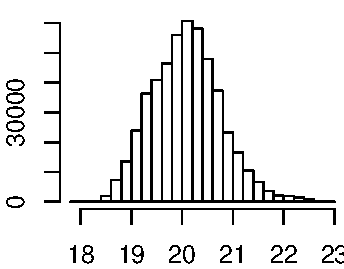
\includegraphics[width=5cm]{calib11}
	}
	\\
	\subcaptionbox{Factor loadings estimated distribution}{
		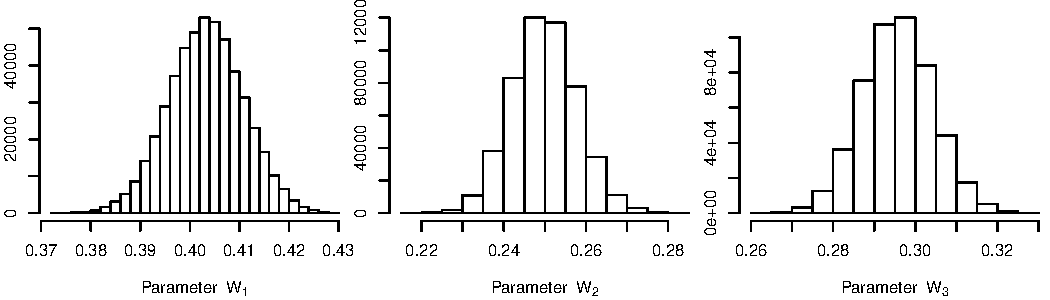
\includegraphics[width=0.98\textwidth]{calib12}
	}
	\\
	\subcaptionbox{Factor correlations estimated distribution}{
		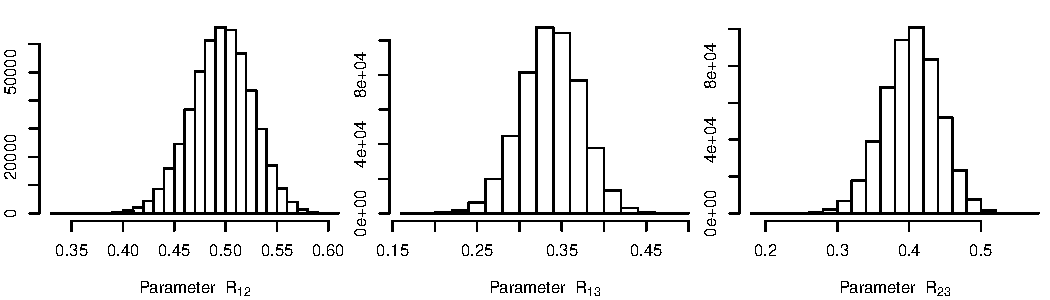
\includegraphics[width=0.98\textwidth]{calib13}
	}
	\caption{Model parameters estimation (1000 obs.)}
	\label{fig:calib1}
\end{figure}

\begin{figure}[!h]
	\centering
	\subcaptionbox{Simulated defaults}{
		%\small
		\begin{tabular}{cc|c|c||c|c||c|c|}
			\cline{3-8}
			& & \multicolumn{6}{|c|}{K (\# defaults)} \\
			\cline{3-8}
			& & \multicolumn{2}{|c||}{S1} & \multicolumn{2}{|c||}{S2} & \multicolumn{2}{|c|}{S3} \\
			\cline{1-1} \cline{3-8}
			\multicolumn{1}{|c|}{Obs} & & A & B & A & B & A & B \\
			\cline{1-1} \cline{3-8}
			\multicolumn{1}{|c|}{1} & & 1 & 14 & 11 & 50 & 11 & 14 \\
			\cline{1-1} \cline{3-8}
			\multicolumn{1}{|c|}{2} & & 2 & 67 & 8 & 26 & 3 & 10 \\
			\cline{1-1} \cline{3-8}
			\multicolumn{1}{|c|}{\vdots} & & \vdots & \vdots & \vdots & \vdots & \vdots & \vdots \\
			\cline{1-1} \cline{3-8}
			\multicolumn{1}{|c|}{20} & & 24 & 190 & 35 & 84 & 65 & 50 \\
			\cline{1-1} \cline{3-8}
		\end{tabular}
	}
	\hfill
	\subcaptionbox{$\nu$ estimated distribution}{
		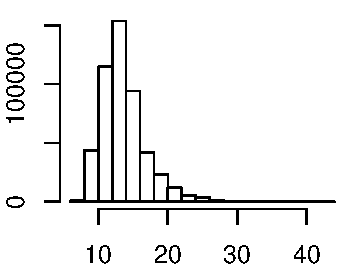
\includegraphics[width=5cm]{calib31}
	}
	\\
	\subcaptionbox{Factor loadings estimated distribution}{
		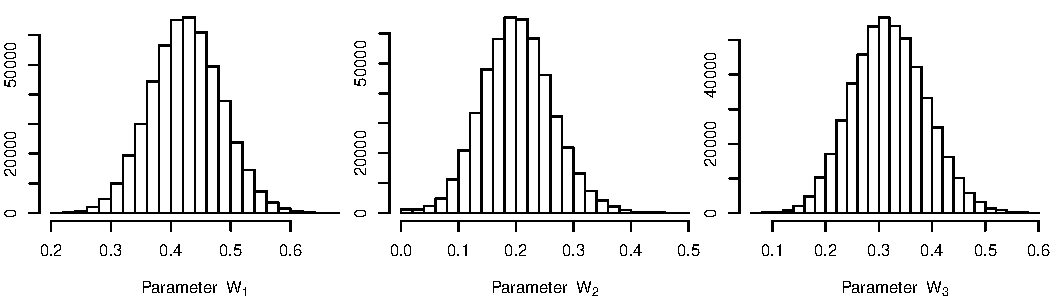
\includegraphics[width=0.98\textwidth]{calib32}
	}
	\\
	\subcaptionbox{Factor correlations estimated distribution}{
		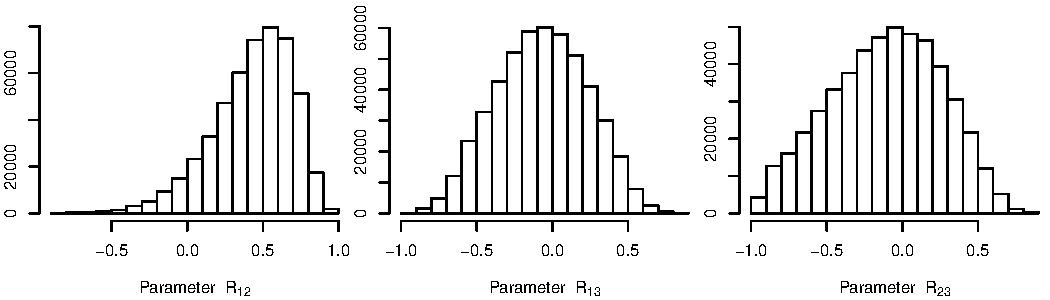
\includegraphics[width=0.98\textwidth]{calib33}
	}
	\caption{Model parameters estimation (20 obs.)}
	\label{fig:calib3}
\end{figure}

\begin{comment}
# R script to generate ccbinf input files
source('/home/gerard/projects/ccbinf/bin/ccbinf.R')
w = c(0.4, 0.25, 0.3)
R = matrix(ncol=3, nrow=3, data=c(1.0,0.5,0.3, 0.5,1.0,0.4, 0.3,0.4,1.0))
nu = 20

p1 = c(0.02, 0.08)
D1 = matrix(ncol=2, nrow=3, data=c(250, 500, 750, 750, 500, 250))
rcount1 = ccruncher.rcount(1000, p1, D1, w, R, nu)
export(rcount1, "calib1.txt")

D2 = diag(apply(D1,1,sum))
p2 = (D1%*%p1)/diag(D2)
rcount2 = rcount1
rcount2$D = D2
rcount2$p = p2
rcount2$K = matrix(nrow=1000, ncol=3*3, 0)
rcount2$K[,1] = rcount1$K[,1] + rcount1$K[,2]
rcount2$K[,5] = rcount1$K[,3] + rcount1$K[,4]
rcount2$K[,9] = rcount1$K[,5] + rcount1$K[,6]
export(rcount2, "calib2.txt")

rcount3 = rcount1
rcount3$K = rcount1$K[1:20,]
rcount3$Z = rcount1$Z[1:20,]
rcount3$S = rcount1$S[1:20]
export(rcount3, "calib3.txt")

quit(save='no')

# bash commands
/home/gerard/projects/ccbinf/build/ccbinf -n 500000 -r 1000 calib1.txt
/home/gerard/projects/ccbinf/build/ccbinf -n 500000 -r 1000 calib2.txt
/home/gerard/projects/ccbinf/build/ccbinf -n 500000 -r 1000 calib3.txt
\end{comment}

\textbf{Averaged PDs}. We may be tempted to consider an averaged PD by sector 
when we lack data disaggregated by rating. The tests we have conducted 
indicate that in the Gaussian case ($\nu = \infty$), this could be an option 
because the estimated parameters using the averaged PDs approximately match 
the expected values. By contrast, when $\nu \ne \infty$, this does not work. 
In example~\ref{ex:calib}, the averaged 1-year PDs by sectors are
\begin{displaymath}
	\begin{array}{lll}
		p_{S_1} = \frac{250}{1000} \cdot p_A + \frac{750}{1000} \cdot p_B = 6.5\% & \quad & N_{S_1} = 250 + 750 = 1000 \\
		p_{S_2} = \frac{500}{1000} \cdot p_A + \frac{500}{1000} \cdot p_B = 5.0\% & \quad & N_{S_2} = 500 + 500 = 1000 \\
		p_{S_3} = \frac{750}{1000} \cdot p_A + \frac{250}{1000} \cdot p_B = 3.5\% & \quad & N_{S_3} = 750 + 250 = 1000 \\
	\end{array}
\end{displaymath}

\textbf{Constrained model}. When we have a significant number of factors 
(e.g., 10) and a reduced set of observations (e.g., 20), then the uncertainty 
of the factor correlation matrix can be high. In these cases, one may consider 
a constrained model~\cite{roncalli:2004} that assumes that all factor 
correlations have the identical value or similar assumptions that reduce the 
number of correlations from which to estimate $s{\times}(s-1)/2$ to only a 
few.
% \begin{displaymath}
% 	R = \left(
% 	\begin{array}{cccc}
% 		     1 &   \rho & \cdots &   \rho \\
% 		  \rho &      1 & \ddots & \vdots \\
% 		\vdots & \ddots & \ddots &   \rho \\
% 		  \rho & \cdots &   \rho &      1 \\
% 	\end{array}
% 	\right)
% \end{displaymath}

\textbf{Degrees of freedom}. We observed that factor correlations and degrees 
of freedom are interwoven. When we fix one of them with a value more distinct 
than generated data and we estimate the other one, the latter reacts to 
compensate for the modification. This effect is more pronounced when the 
number of observations is reduced and the amount of 
information available is scarce, causing the estimations of $\nu$ and $R$
to have a high uncertainty. The Gaussian case ($\nu = \infty$) avoids this 
problem and reduces the number of parameters to estimate (we do not need to 
estimate $\nu$ and $\upsilon^t$ in which $t=1,\dots,T$). 
The risk analyst must evaluate the appropriateness of the Gaussian model 
considering the amount of information available, the number of factors, 
the renounce to capture the tail dependence, the Deviance Information 
Criterion (DIC) values, etc.


%==============================================================================
% MODELING PORTFOLIO LOSS
%==============================================================================
\chapter{Modeling Portfolio Loss}

%------------------------------------------------------------------------------
% PORTFOLIO LOSS DISTRIBUTION
%------------------------------------------------------------------------------
\section{Portfolio Loss Distribution}
\label{sec:pld}

Figure~\ref{fig:lnlblock} displays the hierarchy of the portfolio components.
As we observed in chapter~\ref{chap:mdt}, each obligor belongs to a single 
sector/factor and has a PD with the distribution $F_i$, depending on its 
rating. CCruncher considers that obligors' default times distribution has 
marginals $F_i$ and a t-Student multi-factor copula with $\nu$ degrees of 
freedom, factor loadings $\vec{w}$, and factor correlation matrix $R$.

\begin{figure}[!ht]
	\setlength{\unitlength}{0.14in}
	\centering
%\fcolorbox{red}{yellow}{
	\begin{picture}(33,7)
		\put(0,2){\framebox(6,3){\small Portfolio}}
		\put(9,2){\framebox(6,3){\small Obligor}}
		\put(18,2){\framebox(6,3){\small Asset}}
		\put(27,0){\framebox(6,3){\small LGD(t)}}
		\put(27,4){\framebox(6,3){\small EAD(t)}}
    
		\put(6,3.5){\vector(1,0){3}}
		\put(15,3.5){\vector(1,0){3}}
		\put(24,3){\line(1,0){1}}
		\put(25,3){\line(0,-1){1.5}}
		\put(25,5.5){\vector(1,0){2}}

		\put(24,4){\line(1,0){1}}
		\put(25,4){\line(0,1){1.5}}
		\put(25,1.5){\vector(1,0){2}}
    
		\put(6.5,4){\small 1:n}
		\put(15.5,4){\small 1:n}
		\put(25,6){\small 1:1}
		\put(25,0.5){\small 1:1}
	\end{picture}
%}
	\caption{Hierarchy of the portfolio components}
	\label{fig:lnlblock}
\end{figure}

We define the EAD and LGD concepts used to model the credit risk emphasizing 
the temporal dimension. These concepts and the PD defined in 
section~\ref{ap:pd} are those of the Basel II accord~\cite{basel2:2006}, 
the de-facto international financial risk regulation framework. 

\begin{definition}[Exposure at Default (EAD)]
	The Exposure at Default of the j-th asset of the i-th obligor at time $t$
	indicates the total amount that the bank is exposed if the obligor defaults:
	\begin{displaymath}
		\text{EAD}_i^j(t) = \left\{
		\begin{array}{c}
			\text{amount in risk of the j-th asset of the i-th obligor} \\
			\text{if this defaults at time $t$, measured in currency}
		\end{array}
		\right\}
	\end{displaymath}
	$\text{EAD}_i^j$ can be a function dependent of time when these amounts 
	are fixed and known in advance (e.g., loan, bond) or can be a distribution
	defined over time when we have a model that supports it 
	(e.g., line of credit).
\end{definition}

\begin{definition}[Loss Given Default (LGD)]
	The Loss Given Default of the j-th asset of the i-th obligor at time $t$ 
	indicates the percentage of effective loss over the total exposure. This
	value depends on endorsements, guarantees, type of asset, default time, etc.
	\begin{displaymath}
		\text{LGD}_i^j(t) = \left\{
		\begin{array}{c}
			\text{percentage of the $\text{EAD}_i^j(t)$ that is definitively} \\
			\text{lost if the i-th obligor defaults at time $t$}
		\end{array}
		\right\}
	\end{displaymath}
	$\text{LGD}_i^j$ can be a function dependent of time or can be a 
	distribution defined over time when we have a model that supports it. 
\end{definition}

\begin{example}[10-year Bond]
	Assume a 10-year, fixed-rate bond with an annual coupon of $4\%$ issued 
	by a company rated BB\@. The EAD for this asset can be obtained from its 
	expected cash flow because it is known in advance. We suppose that the 
	bank's internal models indicate that in this case the LGD is a 
	$\text{Beta}(5,2)$ distribution regardless of the default time.
	Figure~\ref{figure:bond} illustrates the defined concepts applied 
	to this asset.
\end{example}

\begin{figure}[!ht]
	\centering
	\subcaptionbox{Exposure at Default}{
		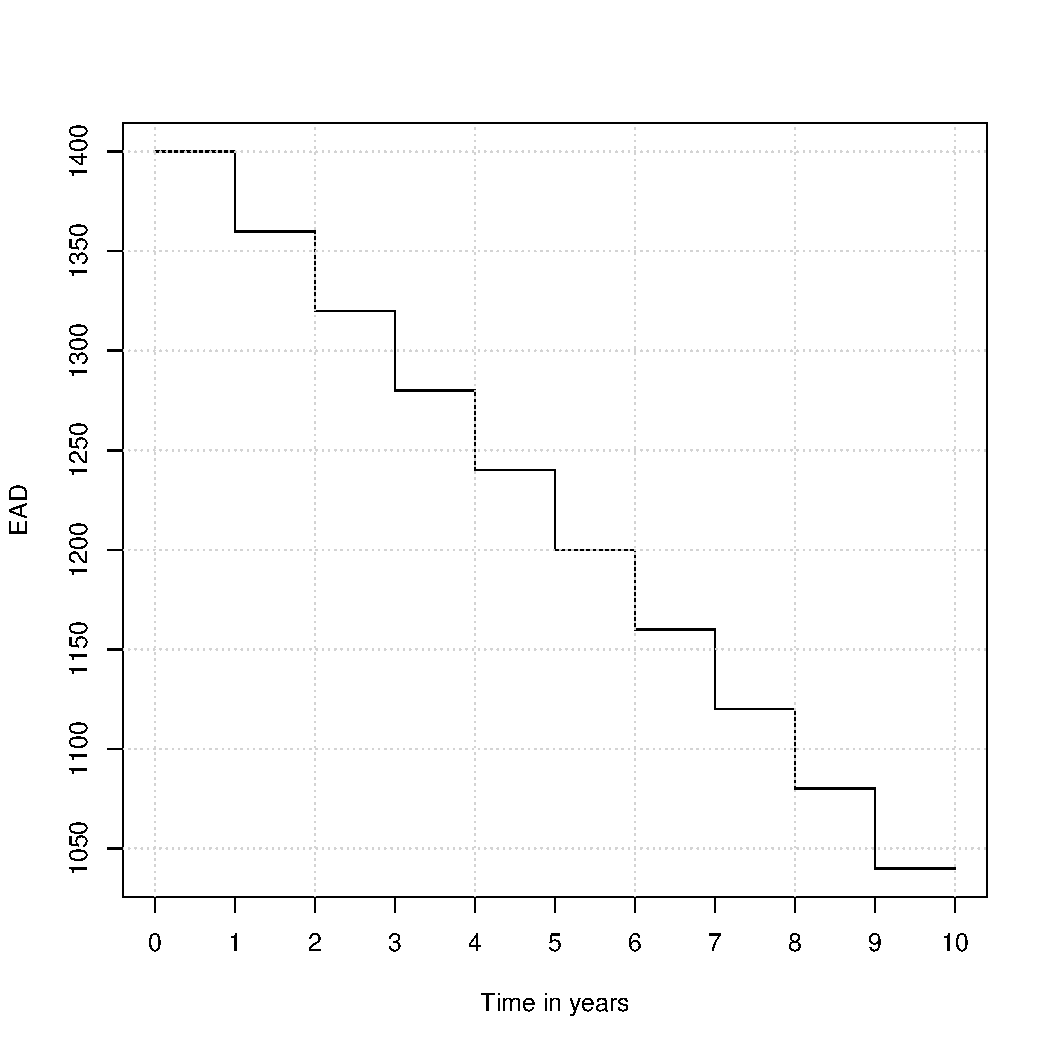
\includegraphics[width=7cm]{bond_ead}
	}
	\subcaptionbox{Loss Given Default}{
		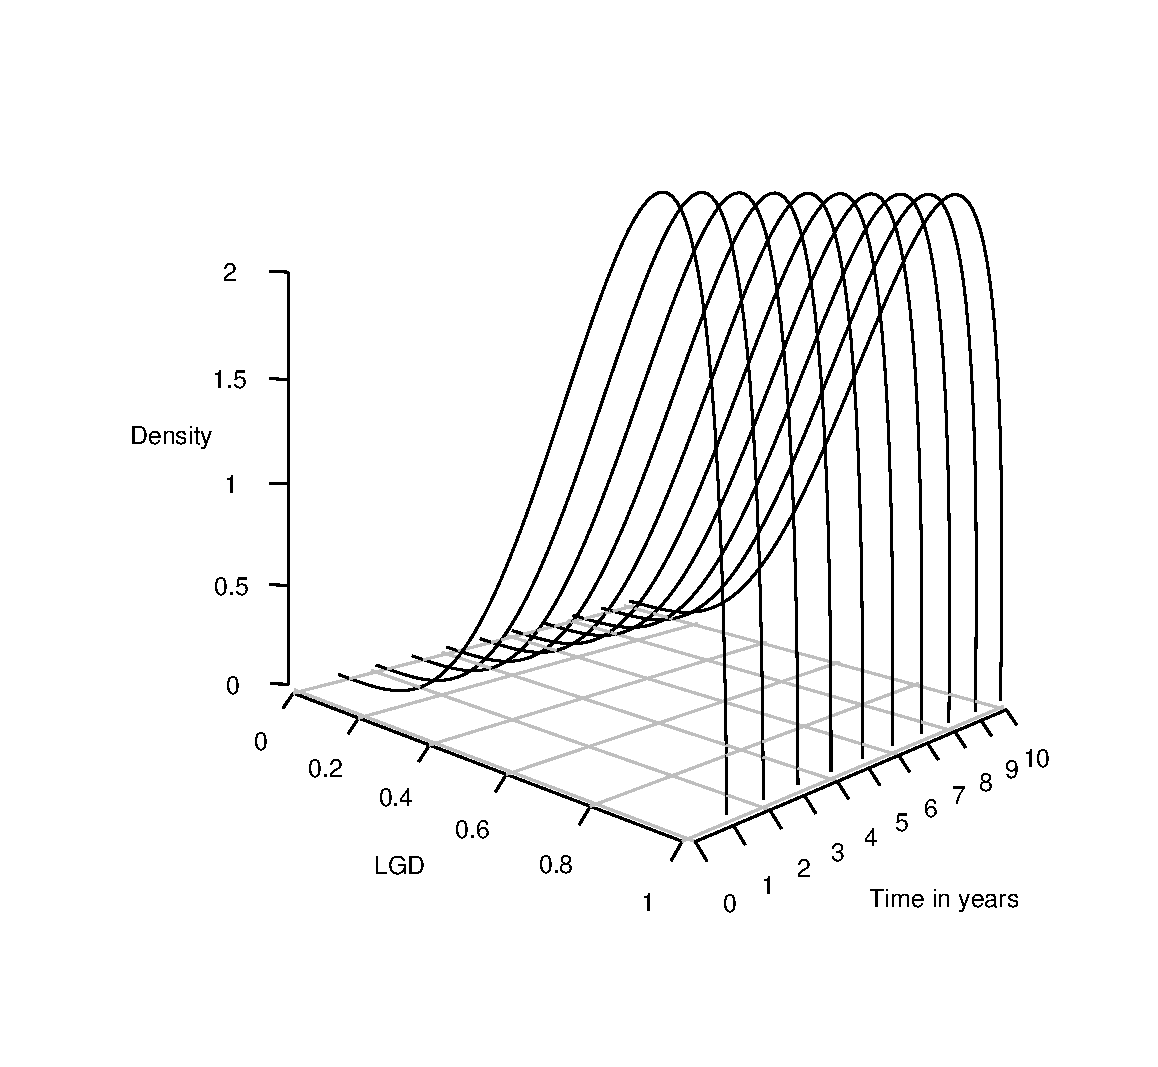
\includegraphics[width=7cm]{bond_lgd}
		\vspace{11pt}
	}
	\caption{10-year bond example}
	\label{figure:bond} 
\end{figure}

\begin{definition}[Portfolio Loss at time $T$]
	The Portfolio Loss at time $T$ is the accumulated losses in the time 
	range $[0,T]$ caused by obligors that default (fail to make payments 
	that they are obligated to make).
	\begin{displaymath}
		L_T = \left\{
		\begin{array}{c}
			\text{sum of portfolio losses in time range $[0,T]$}
		\end{array}
		\right\}
	\end{displaymath}
\end{definition}

Assume a credit portfolio in which the obligors' default times 
$(T_1,\dots,T_n)$ is a multivariate distribution. In addition, we consider 
that each i-th obligor has $m_i$ assets with known EAD and LGD\@. Thus, 
the portfolio loss distribution at time horizon $t$ is
\begin{displaymath}
	L_t = \displaystyle \sum_{i=1}^n \mathbbm{1}_{[0,t]}(T_i) \cdot 
	\left( 
	\sum_{j=1}^{m_i} \text{EAD}_i^j(T_i) \cdot \text{LGD}_i^j(T_i)
	\right)
\end{displaymath}

The portfolio loss distribution $L_t$ does not have a closed form except 
in a few cases. One of those cases is the Large Homogeneous Pool (LHP).
Vasicek~\cite{vasicek:1987} developed an analytical formula in the Gaussian 
case for the loss distribution of an infinitely large portfolio. Later, 
Schloegl and O'Kane~\cite{schloegl:2005} extended the formula to the 
t-Student case. The assumptions of these approximations are 
\begin{inparaenum}[1)]
	\item a one-factor model, 
	\item an infinitely large portfolio, 
	\item equal PDs, and
	\item equal exposure.
\end{inparaenum}
These simplified models must be managed with care because they can cause 
problems~\cite{long:2012} when the assumptions are not realized.

CCruncher assumes that the multivariate default times distribution has
marginals $F_i$ and a t-Student multi-factor copula with degrees 
of freedom $\nu$, factor loadings $\vec{w}$, and factor correlation matrix 
$R$. CCruncher generates samples of the portfolio loss distribution simulating 
the obligors' default times. Portfolio loss distribution is approximated by the 
empirical distribution of the sample, and credit risk is measured using the 
appropriate statistics.

\begin{algorithm}[Portfolio losses sampling]
	\label{alg:pldmc}
	Let a portfolio be categorized in $s$ sectors and $r$ ratings.
	Assume a multivariate default times distribution with marginals $F_i$
	and a t-Student multi-factor copula $C_{\nu,\vec{w},R}^{\text{t}}$.
	We can then simulate a sample of size $M$ of the portfolio loss distribution
	at time $T$ by performing the following:
	\begin{enumerate}
		\item Compute the Cholesky decomposition of $R = L \cdot L^\intercal$
		\item For $m=1,\dots,M$ repeat the following steps:
		\begin{itemize}
			\item $\text{Loss}^m = 0$
			\item Simulate $s$ independent $N(0,1)$, $\vec{y}$
			\item Simulate factors doing $\vec{z} = L \cdot \vec{y}$
			\item Simulate $\upsilon \sim \chi_{\nu}^2$
			\item For each obligor $i=1,\dots,n$ repeat the following steps:
			\begin{itemize}
				\item Set $si = $ i-th obligor sector index
				\item Set $ri = $ i-th obligor rating index
				\item Simulate $\epsilon \sim N(0,1)$
				\item Compute $x_i = \sqrt{\frac{\nu}{\upsilon}} \cdot \left( w_{si} \cdot z_{si} + \sqrt{1-w_{si}^2} \cdot \epsilon \right)$
				\item Compute $t_i = F_{ri}^{-1}\left(t_{\nu}(x_i)\right)$
				\item if $t_i \le T$, then for each asset $j$ belonging to i-th obligor
				\begin{itemize}
					\item Evaluate or simulate $\text{EAD}_i^j(t_i)$
					\item Evaluate or simulate $\text{LGD}_i^j(t_i)$
					\item $\text{Loss}^m = \text{Loss}^m + \text{EAD}_i^j(t_i) \cdot \text{LGD}_i^j(t_i)$
				\end{itemize}
			\end{itemize}
			\item print $\text{Loss}^m$
		\end{itemize}
	\end{enumerate}
\end{algorithm}

\begin{example}[Large Homogeneous Pool]
	\label{ex:test04}
	Assume a portfolio composed of \num{1000} exchangeable obligors (with 
	identical ratings and sectors) in which every obligor owes 1\euro\ to 
	1 year, the 1-year default probability is $p=10\%$, and the factor loading 
	is $20\%$. This problem is close to fulfilling the LHP assumptions. 
	In the Gaussian case, the density is~\cite[chap. 2.5]{bluhm:2002}: 
	\begin{displaymath}
		f_{p,w}(x) = 
		\frac{\sqrt{1-w^2}}{w} \cdot \exp\left( 
			\frac{\left(N^{-1}(x)\right)^2}{2} -
			\frac{\left(N^{-1}(p) - \sqrt{1-w^2} \cdot N^{-1}(x)\right)^2}{2 \cdot w^2}
		\right)
	\end{displaymath}
	in which $w$ is the factor loading, $p$ is the probability to a 1-year 
	horizon, and $x \in (0,1)$ represents the percentage of loss in the 
	portfolio. 

	File \texttt{\$CCRUNCHER/samples/test04.xml} contains the CCruncher input
	file of this example. Figure~\ref{fig:test04} displays the theoretical
	distribution provided by the LHP approach and the distribution approximated 
	by CCruncher, which, as expected, are quite similar. If we reduce the number 
	of obligors from \num{1000} to \num{100}, then the LHP assumptions are 
	broken and the distribution provided by the LHP approach fails.
\end{example}
\begin{comment}
	# bash command
	bin/ccruncher-cmd -w -o data/test04-1000 samples/test04-1000.xml
	bin/ccruncher-cmd -w -o data/test04-100 samples/test04-100.xml
\end{comment}

\begin{figure}[!h]
	\centering
	\subcaptionbox{1000 obligors}{
		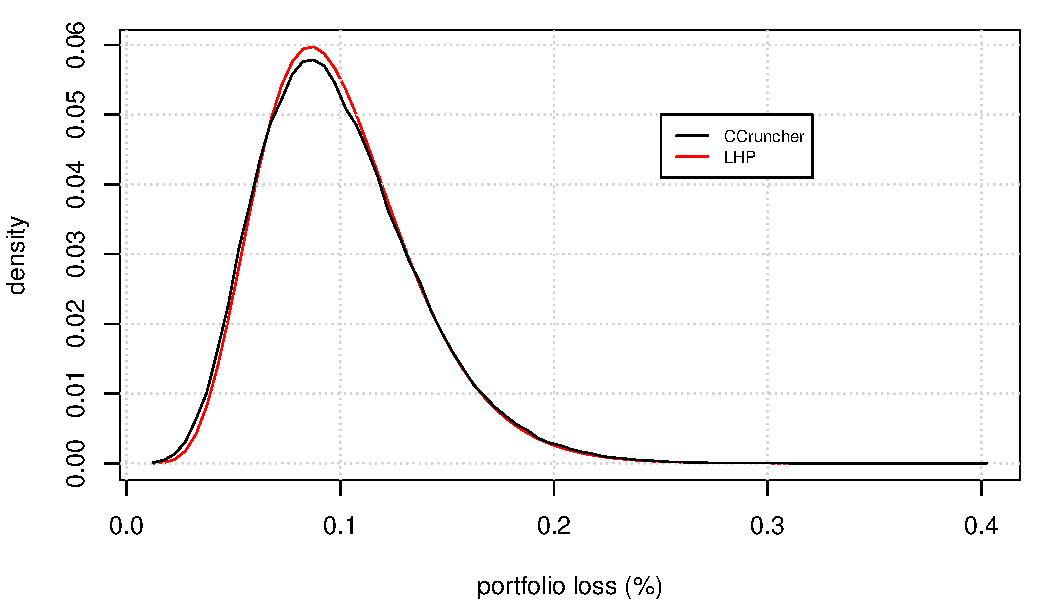
\includegraphics[width=7cm]{test04-1}
	}
	\subcaptionbox{100 obligors}{
		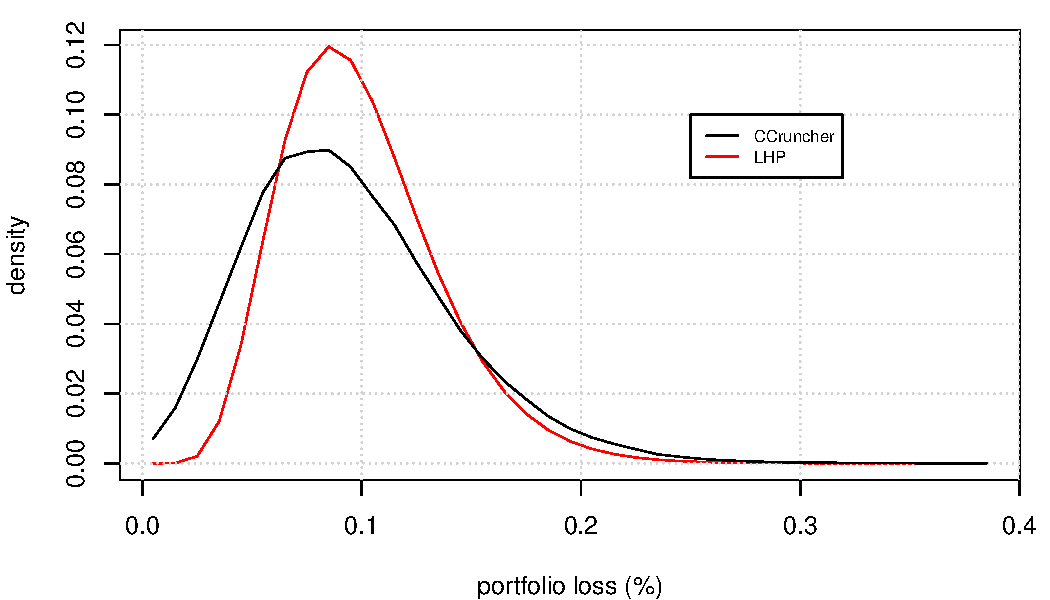
\includegraphics[width=7cm]{test04-2}
	}
	\caption{Large Homogeneous Pool example}
	\label{fig:test04} 
\end{figure}

%------------------------------------------------------------------------------
% CREDIT RISK MEASUREMENT
%------------------------------------------------------------------------------
\section{Credit Risk Measurement}
\label{sec:riskm}

After $N$ simulations (e.g., \num{20000}, \num{500000} or more) of the 
portfolio loss, we measure the portfolio credit risk computing the 
corresponding statistics and their standard errors according to sample size. 

\subsection{Portfolio risk}

In this section we provide the definitions and formulas of the most usual 
credit risk measures. Figure~\ref{fig:lossdistr} illustrates the concepts 
presented in this section. Any other user-defined risk measure can be 
estimated from the simulated sample, and its standard error can be obtained 
using resampling methods.
\begin{figure}[!ht]
	\centering
	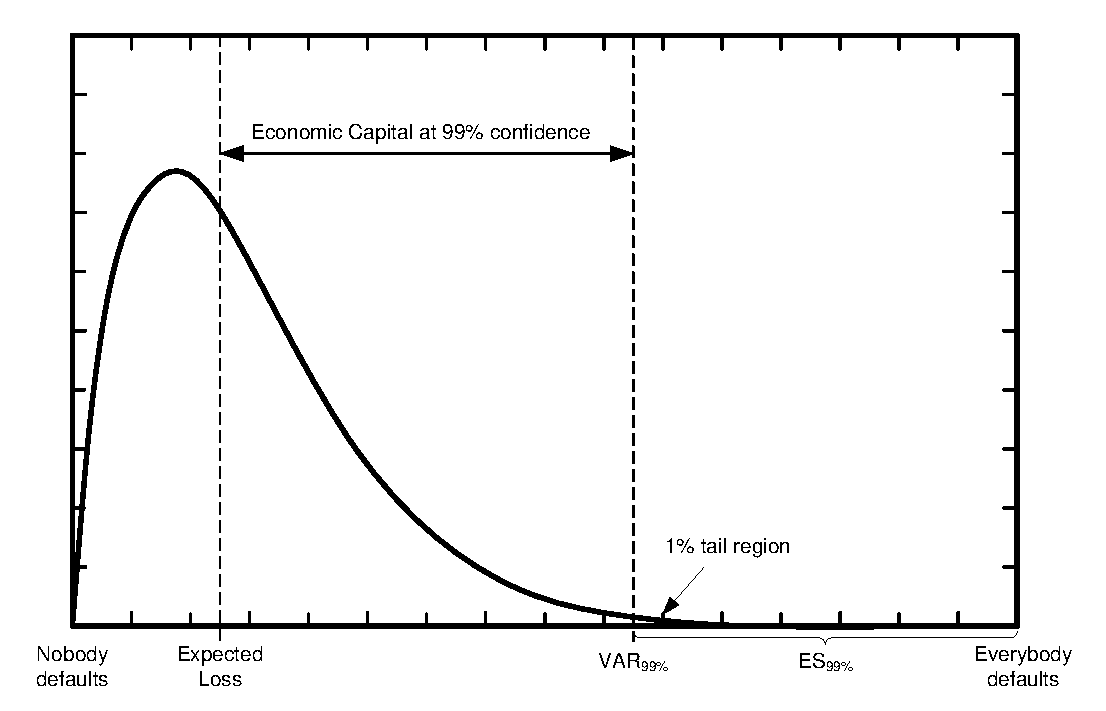
\includegraphics[width=12cm]{creditvar}
	\caption{Portfolio Loss Distribution at time $T$}
	\label{fig:lossdistr}
\end{figure}

% When the loss values are high, for example, $\mathcal{O}(10^7)$, and the 
% number of simulations is also high, for example, $\mathcal{O}(10^6)$, we 
% can incur a loss of precision when we calculate the sum of the squares. 
% The usual manner of storing these values has a 15--17 significant 
% decimal-digit precision that can be exceeded in the sum of squares as we 
% can see in the previous example: $\mathcal{O}(10^{2 \cdot 7 + 6})$. In 
% this case, we recommend using the Kahan~\cite{kahan:1965} summation 
% algorithm.

\subsubsection{Expected Loss}

The Expected Loss attempts to answer the question, ``What is my expected 
loss for the next year?''

\begin{definition}[Expected Loss (EL)]
	The Expected Loss of a portfolio at time horizon $T$ is the 
	mean of the portfolio loss distribution.
	\begin{displaymath}
		\text{EL}(L_T) = E(L_T)
	\end{displaymath}
\end{definition}

Expected Loss can be approximated using the following statistic:

\begin{displaymath}
	\text{EL} = \widehat{\mu} \pm \Phi^{-1}\left(\frac{1-\alpha}{2}\right) \cdot \frac{\widehat{\sigma}}{\sqrt{N}}
	\quad \text{ being } \quad
	\left\{
	\begin{array}{l}
		\displaystyle
		\widehat{\mu} = \frac{1}{N} \sum_{i=1}^{N} x_i \\
		\\
		\displaystyle
		\widehat{\sigma} =
		\sqrt{\frac{1}{N-1} \sum_{i=1}^{N} \left( x_i - \widehat{\mu} \right)^2}
	\end{array}
	\right.
\end{displaymath}
in which $x_i$ are the simulated portfolio losses, $\alpha$ is the error 
confidence level, $\Phi^{-1}$ is the $N(0,1)$ inverse cumulative distribution 
function, and $\widehat{\mu}$ and $\widehat{\sigma}$ are the mean and standard 
deviation estimators.

\subsubsection{Value at Risk}

The Value at Risk~\cite{var:jorion} is the most commonly used risk measure 
to respond to the question, ``How much could I lose in a really bad year?''

\begin{definition}[Value at Risk (VaR)]
	The Value at Risk of a portfolio at time horizon $T$ and confidence level 
	$\beta$ is the $\beta$-quantile of the portfolio loss distribution at time 
	$T$. Consider
	\begin{displaymath}
		\text{VaR}_\beta(L_T) = \inf\{x \in \mathbb{R} \mid F(x) \ge \beta \}
	\end{displaymath}
	in which $F(x)=\Pr\{L_T \le x\}$ is the portfolio loss distribution at 
	time $T$.
\end{definition}

Value at Risk can be approximated using the following statistic:

\begin{displaymath}
	\begin{array}{lcl}
		\textrm{VaR}_{\beta} = \widehat{q_{\beta}} \pm \Phi^{-1}\left(\frac{1-\alpha}{2}\right) \cdot \textrm{stderr}(q_{\beta})
		& \text{ being } &
		\left\{
		\begin{array}{l}
			\displaystyle
			\frac{k}{N} \leq \beta < \frac{k+1}{N} \\
			\\
			\displaystyle
			\widehat{q_{\beta}} = x_{k:N} \\
		\end{array}
		\right.
		\\
		& &
		\\
		\textrm{stderr}(q_{\beta}) = \sqrt{C_2 - C_1^2}
		& \text{ being } &
		\left\{
		\begin{array}{rcl}
			M   & = & [N \cdot \beta + 0.5]  \\
			a   & = & M - 1            \\
			b   & = & N - M            \\
			W_i & = & B(a,b,\frac{i+1}{N}) - B(a,b,\frac{i}{N}) \\
			C_k & = & \sum_{i=1}^{N} W_i \cdot x_i^k \\
		\end{array}
		\right.
		\\
	\end{array}
\end{displaymath}
in which $x_i$ are the simulated portfolio losses, $x_{k:N}$ is the $k$-th 
element of ascendant-sorted values, $\alpha$ is the error confidence level, 
$\Phi^{-1}$ is the $N(0,1)$ inverse cumulative distribution function, 
$\widehat{q_{\beta}}$ is the quantile estimator, $\textrm{stderr}(q_{\beta})$ 
is the estimation of the standard error using the Maritz-Jarrett method 
described in~\cite[chap. 3.5.3]{wilcox:2004}, $[x]$ is the integer part of 
$x$, and $B(a,b,x)$ is the regularized incomplete beta function.
When the sample size is high, the incomplete beta function can be difficult 
to ascertain due to convergence problems. Also, a large sample size causes 
the evaluation of the incomplete beta function multiple being this computation
numerically costly.

\subsubsection{Expected Shortfall}

VaR is not a coherent risk measure because it does not fulfill the 
sub-additive property~\cite{var:varbad}. Expected Shortfall is a coherent 
risk measure similar to VaR~\cite{var:eshortfall}.

\begin{definition}[Expected Shortfall (ES)]
	The Expected Shortfall (aka Conditional VaR, aka Conditional Tail 
	Expectation) of a portfolio at time horizon $T$ and 
	confidence level $\beta$ is the average of the worst $\beta\%$ portfolio 
	losses at time $T$,
	\begin{displaymath}
		\text{ES}_\beta(L_T) = \text{E}(L_T \mid L_T \ge \text{VaR}_\beta(L_T))
	\end{displaymath}
\end{definition}

Expected Shortfall can be approximated using the following statistic:

\begin{displaymath}
	\text{ES}_{\beta} = \widehat{\mu} \pm \Phi^{-1}\left(\frac{1-\alpha}{2}\right) \cdot \frac{\widehat{\sigma}}{\sqrt{K}}
	\quad \text{ being } \quad
	\left\{
	\begin{array}{l}
		\displaystyle
		\widehat{\mu} = \frac{1}{K} \sum_{i=1}^{K} y_i \\
		\\
		\displaystyle
		\widehat{\sigma} =
		\sqrt{\frac{1}{K-1} \sum_{i=1}^{K} \left( y_i - \widehat{\mu} \right)^2}
	\end{array}
	\right.
\end{displaymath}
in which 
$\{y_1, \ldots, y_K\} = \{x_i \mid x_i \ge \text{VaR}_{\beta} \}_{i=1,\dots,N}$ 
are the simulated portfolio losses larger than $\text{VaR}_{\beta}$, 
$\alpha$ is the error confidence level, $\Phi^{-1}$ is the $N(0,1)$ 
inverse cumulative distribution function, and $\widehat{\mu}$ and 
$\widehat{\sigma}$ are the mean and standard deviation estimators.
This estimator assumes that the estimated $\text{VaR}_{\beta}$ has the 
exact value. Despite this, if the sample size is high enough, then the 
estimated value is good enough.

\begin{example}[2 factors]
	\label{ex:test05}
	Assume a portfolio composed of \num{1000} obligors in which every obligor 
	owes 1\euro\ to 1 year. Then $\text{EAD}_i^1(t) = \mathbbm{1}_{[0,1]}(t)$, 
	with a $\text{LGD}_i^1(t)=100\%$. There are 4 ratings \{A, B, C, D\}; D is 
	the \emph{defaulted} status, and the remaining ratings have the following 
	1-year default probability: $p_A = 5\%, p_B = 10\%, p_C = 20\%$. Factor 
	loadings are $\vec{w} = (0.4, 0.35)$, and the factors correlation is 
	$\text{Cor}(S_1,S_2) = 0.25$. The t-Student copula has $\nu=15$ degrees
	of freedom, and the number of obligors by sector and rating are

	\hspace*{1cm}
	\begin{tabular}{|c|c|c||c|c|c|}
		\hline
		\multicolumn{3}{|c||}{S1} & \multicolumn{3}{|c|}{S2} \\
		\hline
		A & B & C & A & B & C \\
		\hline
		167 & 166 & 167 & 167 & 167 & 166 \\
		\hline
	\end{tabular}

	File \texttt{\$CCRUNCHER/samples/test05.xml} contains the CCruncher input
	file of this example. Figure~\ref{fig:test05} displays the portfolio
	loss density and risk measures obtained using \num{200000} values 
	simulated by CCruncher.

	It is difficult to ascertain the validity of this example. Some 
	authors~\cite{cespedes:2002} obtained quasi-analytical expressions for 
	the Gaussian two-factor model with a common PD; however, those expressions 
	are not applicable to this example (t-Student, multiple PDs). One manner in 
	which to check that the result is correct involves disaggregating the 
	simulated portfolio losses by sector-rating (see section~\ref{ss:ra}) and 
	estimating the parameters $\nu, \vec{w}$, and $R$ with the first \num{1000} 
	simulations using the procedure described in section~\ref{sec:binf}. 
	If the estimated parameters match the parameters of the example, we have
	consistent simulation and estimation algorithms. Observe that in 
	this case, the simulated losses can be equated to the number of defaults 
	because each defaulted obligor is computed as a 1\euro\ loss.
\end{example}

\begin{figure}[!h]
	\centering
	\subcaptionbox{Risk measures}{
		%\small
		\begin{tabular}{|l|c|c|}
			\hline
			Statistic & Value & Std. Err. \\
			\hline
			EL & 116.58 & 0.16 \\
			$\text{VaR}_{95\%}$ & 252.00 & 1.09 \\
			$\text{VaR}_{99\%}$ & 338.00 & 2.22 \\
			$\text{VaR}_{99.9\%}$ & 442.00 & 5.44 \\
		
			$\text{ES}_{95\%}$ & 304.63 & 0.49 \\
			$\text{ES}_{99\%}$ & 383.82 & 0.96 \\
			$\text{ES}_{99.9\%}$ & 480.98 & 2.71 \\
		
			\hline
	    \end{tabular}
	}
	\hfill
	\subcaptionbox{Portfolio loss density}{
		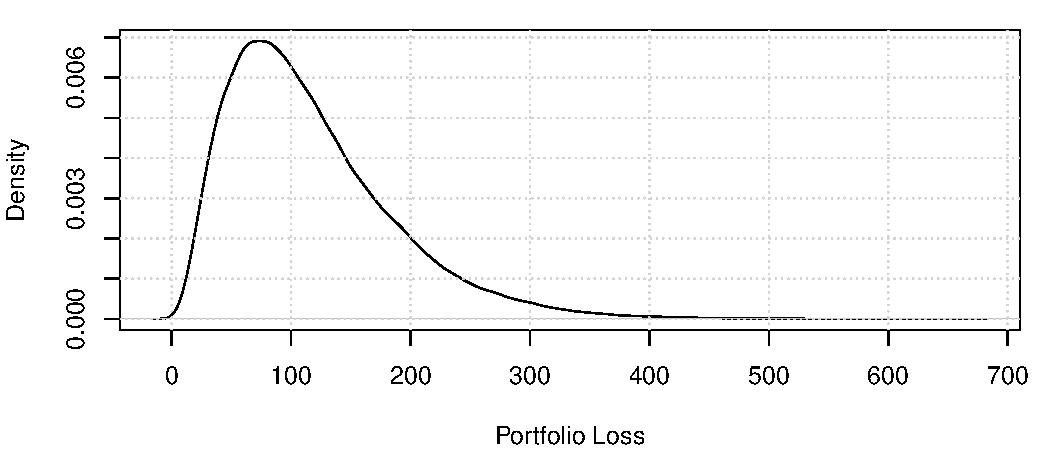
\includegraphics[width=9cm]{test05}
	}
	\caption{2-factors example}
	\label{fig:test05}
\end{figure}

\subsection{Risk Disaggregation}
\label{ss:ra}

Once we have measured the credit risk, naturally arises the question 
``how much of this risk corresponds to the business unit X?'' CCruncher
allows defining and simulating sub-portfolio losses in order to respond
this question.

CCruncher simulates the entire portfolio loss at time $T$. It also allows 
(in the same execution) the simulation of sub-portfolios losses. In CCruncher, 
a sub-portfolio is called a \emph{segment}. The disjoint union of segments 
covering the entire portfolio is called a \emph{segmentation}, i.e., a 
segmentation is composed by non-overlapped segments that constitute the 
entire portfolio. For example, we can define the segmentation of geographic
areas where the bank operates composed by four segments \{N, S, E, W\}.
When an obligor defaults, the loss of its assets is added into the 
entire portfolio loss and into the segment loss where the obligor resides.
CCruncher allows defining and managing multiple segmentations simultaneously. 
The segmentations can be composed of obligors or assets. In the first case, 
the obligor loss is aggregated to segment loss when the obligor defaults. 
In the second case, the asset losses are aggregated to segment losses when 
the obligor defaults.

\begin{figure}[!h]
	\centering
	\subcaptionbox{EL disaggregation}{
		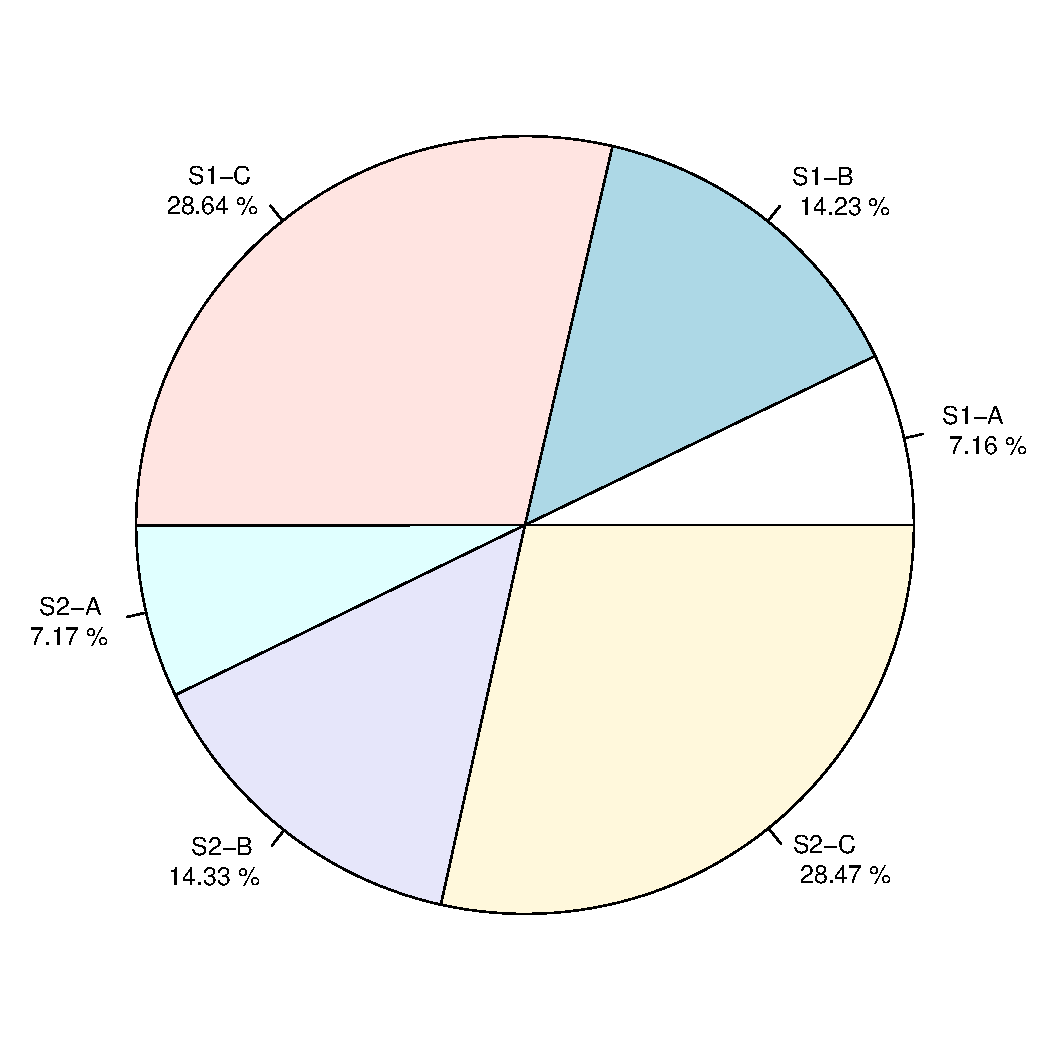
\includegraphics[width=7cm]{disaggregation1}
	}
	\subcaptionbox{$\text{ES}_{99\%}$ disaggregation}{
		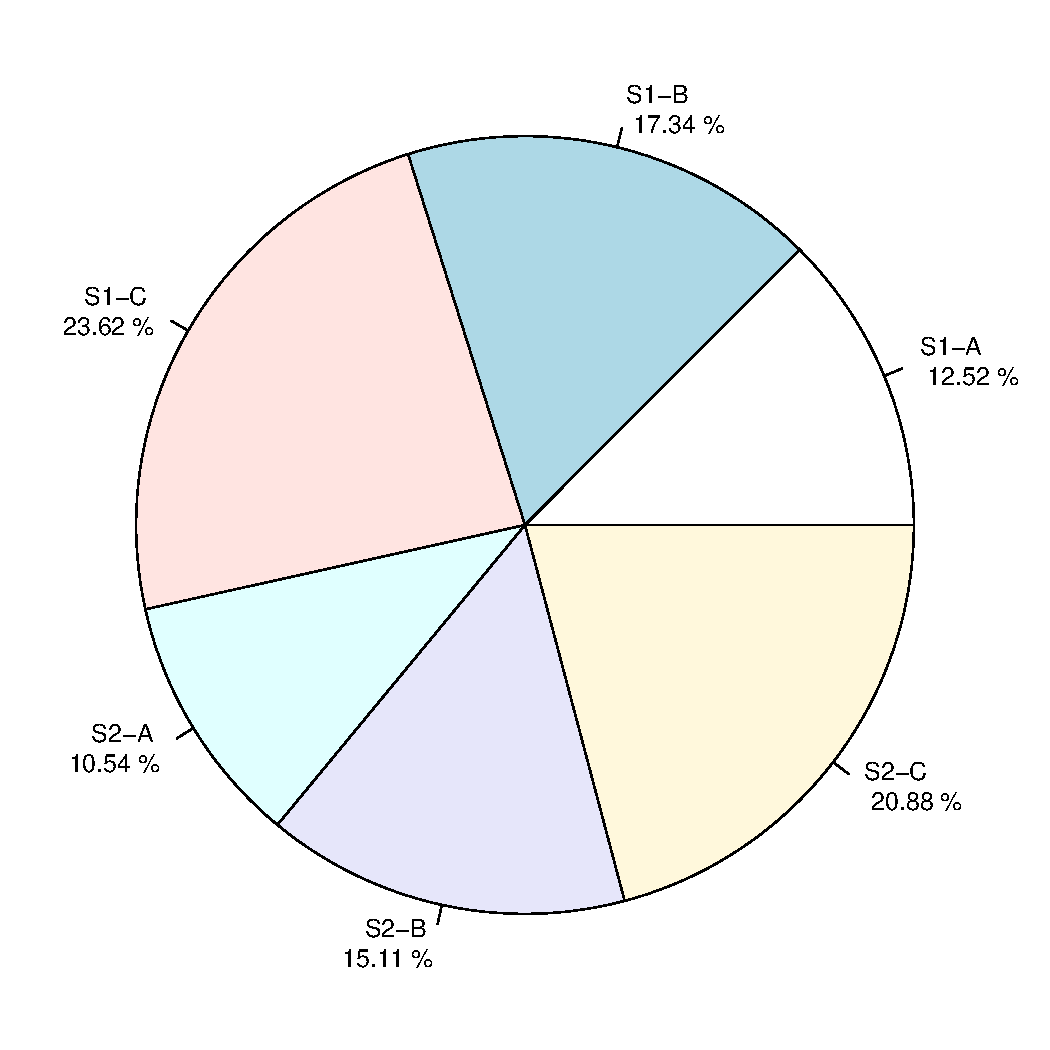
\includegraphics[width=7cm]{disaggregation2}
	}
	\caption{Risk disaggregation}
	\label{fig:disaggregation} 
\end{figure}

\subsubsection{Expected Loss}
Expected Loss is additive respect the portfolio composition, i.e., if 
$L$, $L_1$, and $L_2$ are respectively the portfolio, sub-portfolio 1, 
and sub-portfolio 2 loss distributions in which $L=L_1+L_2$, then 
$\text{EL}(L_1) + \text{EL}(L_2) = \text{EL}(L)$. The EL attributable
to the k-th segment, in cash, is given by the following statistic:
\begin{displaymath}
	\text{EL}_k = \frac{1}{N} \displaystyle \sum_{i=1}^{N} x_i^k
\end{displaymath}
in which $x_i^k$ are the simulated losses of the k-th sub-portfolio.
Dividing $\text{EL}_k$ by the portfolio EL gives the percentage of EL 
consumed by this sub-portfolio.

\subsubsection{Value at Risk}
Value at Risk is not additive, it is not even sub-additive~\cite{var:varbad}.
As mentioned in~\cite[chap. 5.2.2]{bluhm:2002}, calculating VaR risk 
measure contributions is a natural but difficult attempt. In the CCruncher 
case, problems arise when we try to estimate 
$\text{E}\left(L_k \mid L = \text{VaR}_{\beta}(L)\right)$ because the subsample
of simulated sub-portfolio losses having a portfolio loss equal to 
$\text{VaR}_{\beta}$ has a very small size. For this reason, CCruncher 
don't provides support for VaR disaggregation.

\subsubsection{Expected Shortfall}
Expected Shortfall can be disaggregated using the simulated losses of the 
portfolio and its sub-portfolios. As indicated 
in~\cite[chap. 5.2.3]{bluhm:2002}, the contribution of k-th sub-portfolio to 
ES is given by $\text{E}\left(L_k \mid L \ge \text{VaR}_{\beta}(L)\right)$.
The ES attributable to the k-th segment, in cash, is given by the 
following statistic:
\begin{displaymath}
	\text{ES}_k = \frac{1}{K} \displaystyle \sum_{i=1}^{K} y_i^k
\end{displaymath}
in which $x_i$ are the simulates portfolio losses, $x_i^k$ are the simulated 
losses of the k-th sub-portfolio, and
$\{y_1^k,\dots,y_K^k\} = \{x_i^k \mid x_i \ge \text{VaR}_{\beta}\}_{i=1\dots N}$ 
are the simulated sub-portfolio losses having a portfolio loss large than 
$\text{VaR}_{\beta}$.

\begin{example}[Risk disaggregation]
	We use the identical scenario as that described in example~\ref{ex:test05} 
	and that corresponds to CCruncher input file \texttt{test05.xml}. This 
	example defines a segmentation named \emph{sector-rating} with segments 
	S1-A, S1-B, S1-C, S2-A, S2-B, S2-C. Segment X-Y is composed by the obligors 
	located at sector X with the rating Y; each segment has $\approx 166$ 
	obligors. Figure~\ref{fig:disaggregation} displays the risk disaggregated 
	respect this segmentation.
\end{example}

%------------------------------------------------------------------------------
% SIMULATION DETAILS
%------------------------------------------------------------------------------
\section{Simulation Details}

\textbf{Variance reduction}. CCruncher generates random samples from the 
portfolio loss distribution. This sample is used to estimate the risk measures 
(e.g., VaR) using the statistics described in section~\ref{sec:riskm} or any 
other required by the analyst. Any one of these measures, considered 
individually, can be formulated as a Monte Carlo problem and can apply some 
variance reduction techniques (e.g., importance sampling~\cite{brereton:2012}), 
but not simultaneously. For this reason, the variance reduction techniques 
used in CCruncher do not seek an increase in precision, but an improvement 
in the overall results in some manner. The applied variance reduction procedures 
implemented in CCruncher are antithetic variates and Latin hypercube 
sampling. You can found more info at appendix~\ref{ap:vr}.

\emph{Antithetic variates}. In CCruncher the random sampling of the portfolio 
loss distribution is 
performed using $g(X)$ in which $X$ is a multivariate t-Student distribution 
and $g(x) = F^{-1}(t_{\nu}(x))$. We use the fact that the multivariate 
t-Student distribution $X$ is symmetrical, that is, $(x_1,\dots,x_n)$ is 
equiprobable to $(-x_1,\dots,-x_n)$, to apply the antithetic method. 
Expected Loss is the unique statistic that benefits from the variance 
reduction. However, rather than reducing the variance, we are interested 
in the reusing of the simulated random numbers to increase the simulation 
speed. When we use the antithetic method to sample the default times and 
there are some stochastic EADs or LGDs, we use distinct EADs' and LGDs' 
random values for each variate.

\emph{Latin hypercube sampling}. In CCruncher, the random variables that can be 
sampled using the LHS 
technique are the degrees of freedom $\nu$, and the factors $\vec{z}$. 
The aim is to ensure a uniform scanning of these variables so that the
extreme cases are represented.

\textbf{EAD and LGD interpolation}. Given an asset, CCruncher knows its EAD 
and LGD values at fixed times $\{t_1,\dots,t_n\}$ provided by the user. When 
we evaluate these functions in a time value distinct from those provided, we 
use the following piecewise constant interpolation:
\begin{displaymath}
  \left.
	\begin{array}{rcl}
		\text{EAD}(t) & = & \text{EAD}(t_k) \\
		\text{LGD}(t) & = & \text{LGD}(t_k)
	\end{array}
	\right\}
	\quad \text{where} \quad t_{k-1} < t \le t_{k}
\end{displaymath}

\textbf{PD functions approximation}. CCruncher allows defining the PD
functions using the transition matrix or defining explicitly the PD values
at some fixed times. When PDs are defined using the transition matrix, 
CCruncher uses proposition~\ref{prop:pdftm} to derive $F_i$ for each 
month, and intermediate values are interpolated using cubic splines. 
When PDs are defined explicitly at some fixed times, then intermediate 
values are interpolated using cubic splines; however, if the resulting 
function is not strictly increasing, then CCruncher uses linear splines.

\textbf{Function composition}. To speed up the evaluation of the function 
$t=F_r^{-1}(t_{\nu}(x))$ involved in the simulation of obligors' default 
times, we interpolate the function using linear splines on a selected set 
of points $\mathbb{S} = \left\{(x_1,d_1),\dots,(x_k,d_k)\right\}$. 
Let $\{t_1,\dots,t_m\}$ represent the days in which PDs have known values 
(not interpolated), and let $t=P(x)$ represent the function 
$t=F_r^{-1}(t_{\nu}(x))$ linearly interpolated using the current points 
of $\mathbb{S}$. CCruncher determines the set $\mathbb{S}$ using the 
following procedure:
\begin{itemize}
	\item Add the first day of the simulation time range to $\mathbb{S}$, $d_1$.
	\item Add the last day of the simulation time range to $\mathbb{S}$, $d_T$.
	\item Repeat until $\displaystyle \max_{d_1 \le d \le d_T}\left|d - P(t_{\nu}^{-1}(F_r(d)))\right| < 1$ hour
	\begin{itemize}
		\item Let $d$ be the day on which maximum error is achieved
		\item Let $t_i \le d \le t_{i+1}$ be the nearest days on which PDs are user defined
		\item If $t_i$ is not contained in $\mathbb{S}$, add $t_i$ to $\mathbb{S}$
		\item Else if $t_{i+1}$ is not contained in $\mathbb{S}$, add $t_{i+1}$ to $\mathbb{S}$
		\item Else add $d$ to $\mathbb{S}$
	\end{itemize}
\end{itemize}

\textbf{Interest rate}. CCruncher allows considering the Net Present Value 
of the simulated losses. This is computed using an interest rate curve 
defined at fixed times and interpolated using linear or cubic splines 
(selected by user). Allowable methods are simple interest, compound interest 
and continuous interest. The formulas used to compute the present value are
as follows:
\begin{center}
	\begin{tabular}{ccccc}
		$V_0 = \frac{V_t}{1+r \cdot \Delta t}$ & $\qquad$ &
		$V_0 = \frac{V_t}{(1+r)^{\Delta t}}$ & $\qquad$ &
		$V_0 = \frac{V_t}{\exp(r \cdot \Delta t)}$ \\
		(Simple) & $\qquad$ & (Compound) & $\qquad$ & (Continuous)
	\end{tabular}
\end{center}
in which $V_t$ is the value at time $t$ and $r$ is the interest rate given 
by the interest curve at time $t$. Don't consider this option if your EADs
are the sum of cash flow on distinct dates. In this case, we recommend 
filling the input file with the EADs' present value and setting to $0$ the 
interest rate curve.

\textbf{Parallel computing}. 
CCruncher parallelizes the portfolio loss sampling, spawning multiple 
simulation threads, each with its own Mersenne twister Random Number 
Generator seeded with consecutive values. When the number of obligors is 
high, data do not fit in the cache memory L1 and L2. The memory transfer is 
a time-consuming operation that must be minimized. To achieve this, a CCruncher 
threads perform simultaneously \emph{blocksize} simulations. Each obligor is 
simulated \emph{blocksize} times (each of them with the corresponding $\nu$ 
and $\vec{z}$) before moving to the next obligor.

\textbf{Parameterization}. 
The CCruncher input file contains the data required to simulate the portfolio
losses (obligors, assets, EADs, LGDs, ratings, factor correlations, factor
loadings, copula to use, interest rates, segmentations, etc.). This file can 
be quite large (e.g., 1GB). When we evaluate the risk sensitivity or the effect 
of parameters' uncertainty, we must slightly modify the input file and 
reevaluate the portfolio loss distribution multiple times. To simplify this 
task, CCruncher provides the macro mechanism, that allows using variables 
that are replaced by the user-defined values anywhere they are located in 
the input file, and the automatic evaluation of numerical expressions. 
Combining these two features, macros and the evaluation of numerical 
expressions, provides a flexible manner in which to parameterize one's input 
file (e.g., 2000*\$EUR2USD). 


%==============================================================================
% ADDITIONAL TOPICS
%==============================================================================
\chapter{Additional Topics}

%------------------------------------------------------------------------------
% RISK SENSITIVITY
%------------------------------------------------------------------------------
\section{Risk Sensitivity}

In this section we make a basic sensitivity analysis evaluating the variation 
of a parameter $s$, in the risk measure $V$. The goal is to determine the 
appearance of the curve $V(s)$ (increasing/decreasing, concave/convex, 
linear/quadratic/logarithmic, asymptotic behavior) and an estimate of the 
slope given by $\frac{\partial V}{\partial s}$.

It is difficult to draw general guidelines in the absence of a closed formula 
for the portfolio credit risk that takes into account all the parameters: 
number of ratings, PDs over time, number of sectors, number of obligors, EADs 
and LGDs for each asset, factor loadings, factor correlations, and $\nu$. For 
this reason, we lays out this section analyzing the case \texttt{test05.xml} 
exposed in example~\ref{ex:test05}. In this case, we consider that risk 
measure is $\text{ES}_{99\%}$ and parameters subject to sensibility analysis 
are: $n, \vec{w}, R, \nu$.

We sketch the function $\text{ES}_{99\%}(s)$ by calculating $\text{ES}_{99\%}$ 
in various consecutive values of the analyzed parameter. Each of these values 
is obtained by applying the simulation procedure described in Chapter 4. 
In order to reduce variations caused by the simulation procedure, we use the 
same RNG seed in each evaluation.

\begin{example}[Sensitivity to portfolio size]
	Common sense tells us that a large and homogeneous portfolio must have the 
	same risk (as percentage of the total exposure) that a portfolio with the 
	same characteristics but with twice obligors. Figure~\ref{fig:sensi1}
	shows the $\text{ES}_{99\%}$ by varying the number of obligors that 
	compose the portfolio described in \texttt{test05.xml}. Note that this
	value is almost equal in range $[200,\infty)$. In the range $[50,200]$
	we can appreciate the impact of the small number of individuals in the 
	risk measure, not very exaggerated otherwise.
\end{example}

\begin{figure}[!ht]
	\centering
	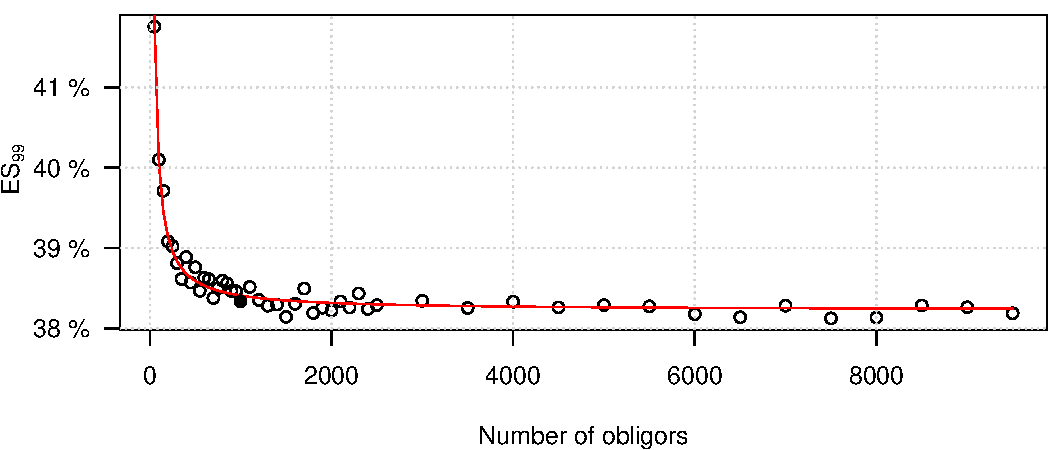
\includegraphics[width=0.98\textwidth]{sensi-size}
	\caption{$\text{ES}_{99\%}$ vs. portfolio size}
	\label{fig:sensi1}
\end{figure}

\begin{example}[Sensitivity to copula parameters]
	Figure~\ref{fig:sensi2} shows the portfolio risk value $\text{ES}_{99\%}$ 
	depending on the copula parameters. Each dot is a 
	risk value computed using a simulation, the black dot corresponds to the 
	original value in example~\ref{ex:test05}, and the confidence bounds shows 
	the impact of the parameter value in the error attributable to simulation 
	(this value is magnified in order to appreciate the impact).
	
	If we consider only the range of feasible values (eg. $w_i \in (0,0.5)$, or
	$\nu \in (5,\infty)$), we note that the impact of factor loading loadings
	and $\nu$ are similar. However, the impact of factor correlations is much 
	smaller. This is good news, because as we saw in the estimation of the 
	parameters, the uncertainty of factor correlations is much higher than 
	that of factor loadings. We also recall that in the estimation procedure,
	the values of factor loadings and $\nu$ are interlaced. 
\end{example}

\begin{figure}[!h]
	\centering
	\subcaptionbox{Parameter $w_1$}{
		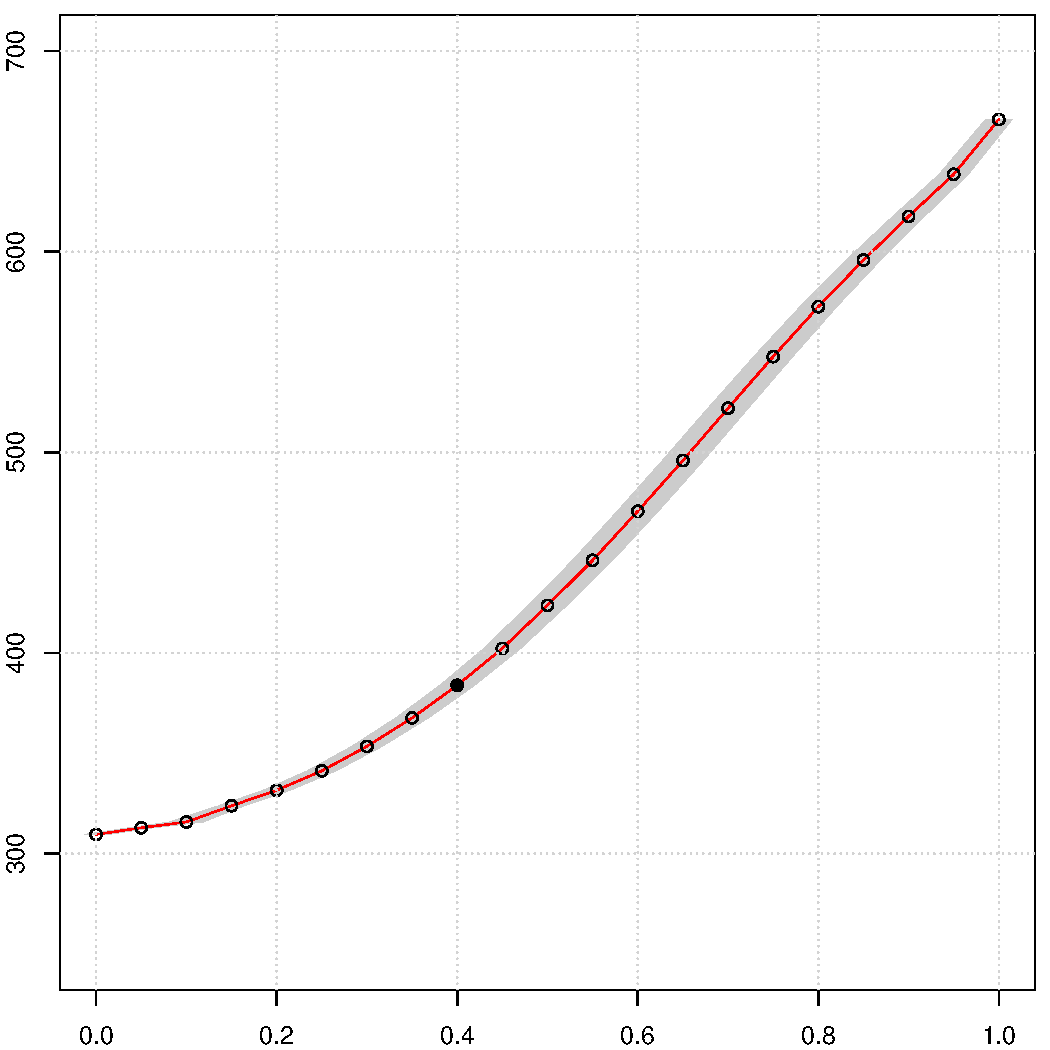
\includegraphics[width=7cm]{sensi-w1}
	}
	\subcaptionbox{Parameter $w_2$}{
		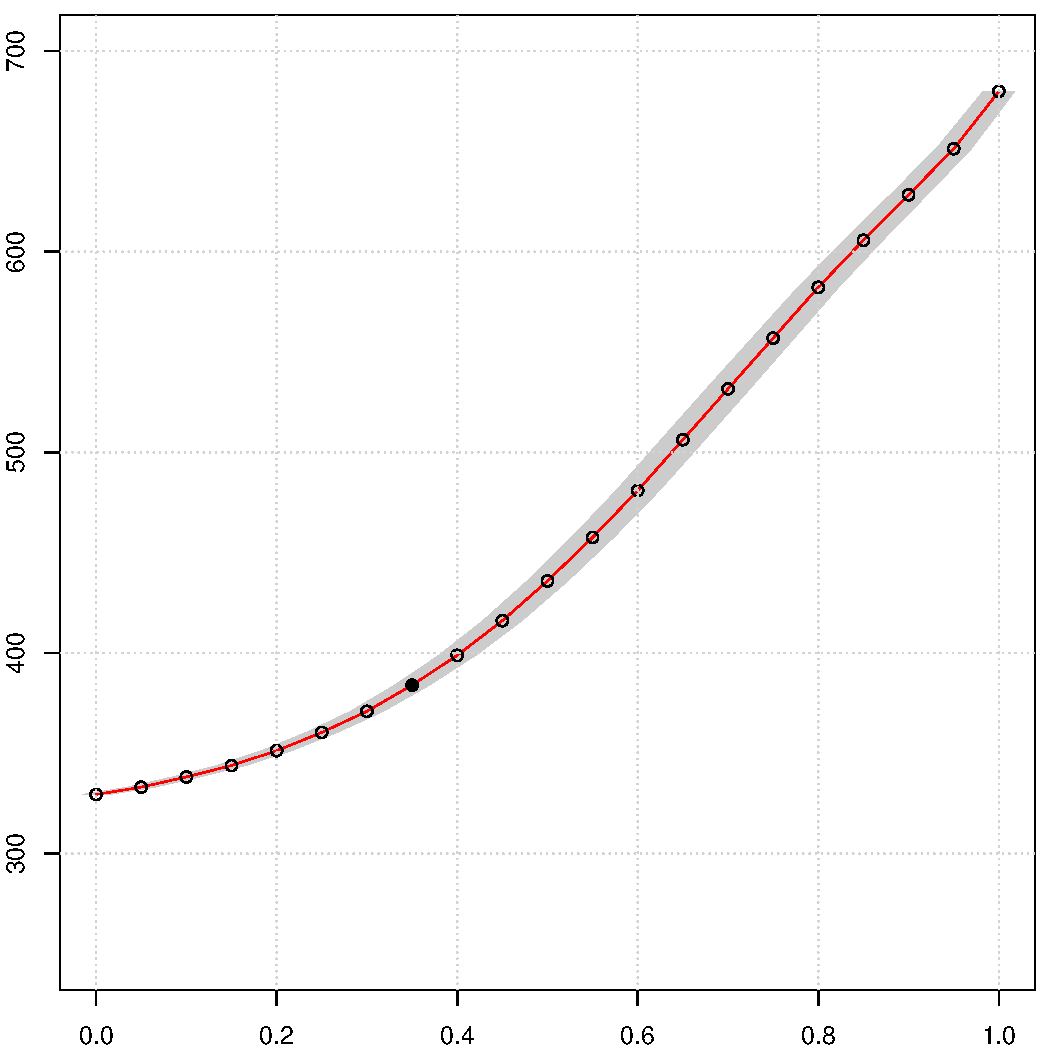
\includegraphics[width=7cm]{sensi-w2}
	}
%	\caption{$\text{ES}_{99\%}$ sensitivity to factor loadings}
%	\label{fig:sensi2}
	\\
	\subcaptionbox{Parameter $R_{12}$}{
		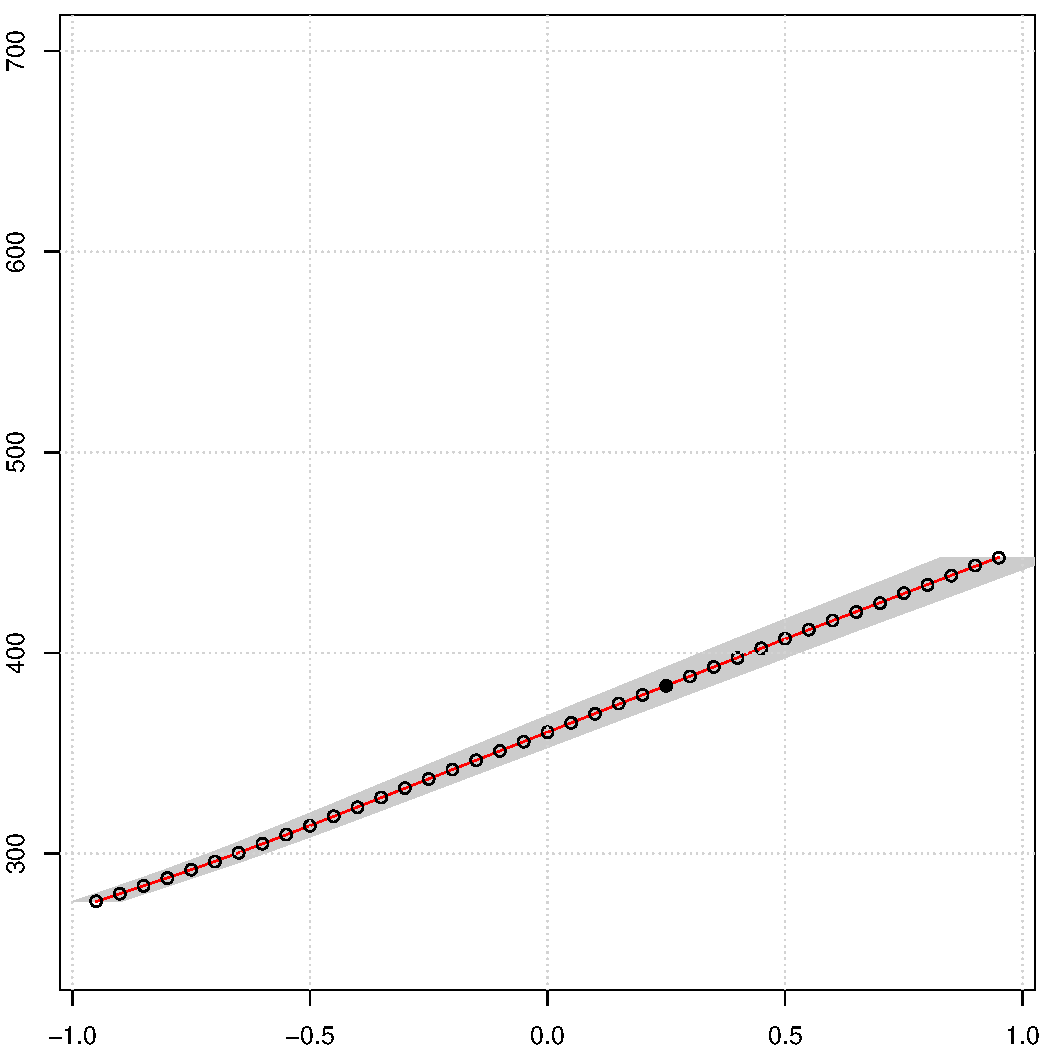
\includegraphics[width=7cm]{sensi-r12}
	}
	\subcaptionbox{Parameter $\nu$}{
		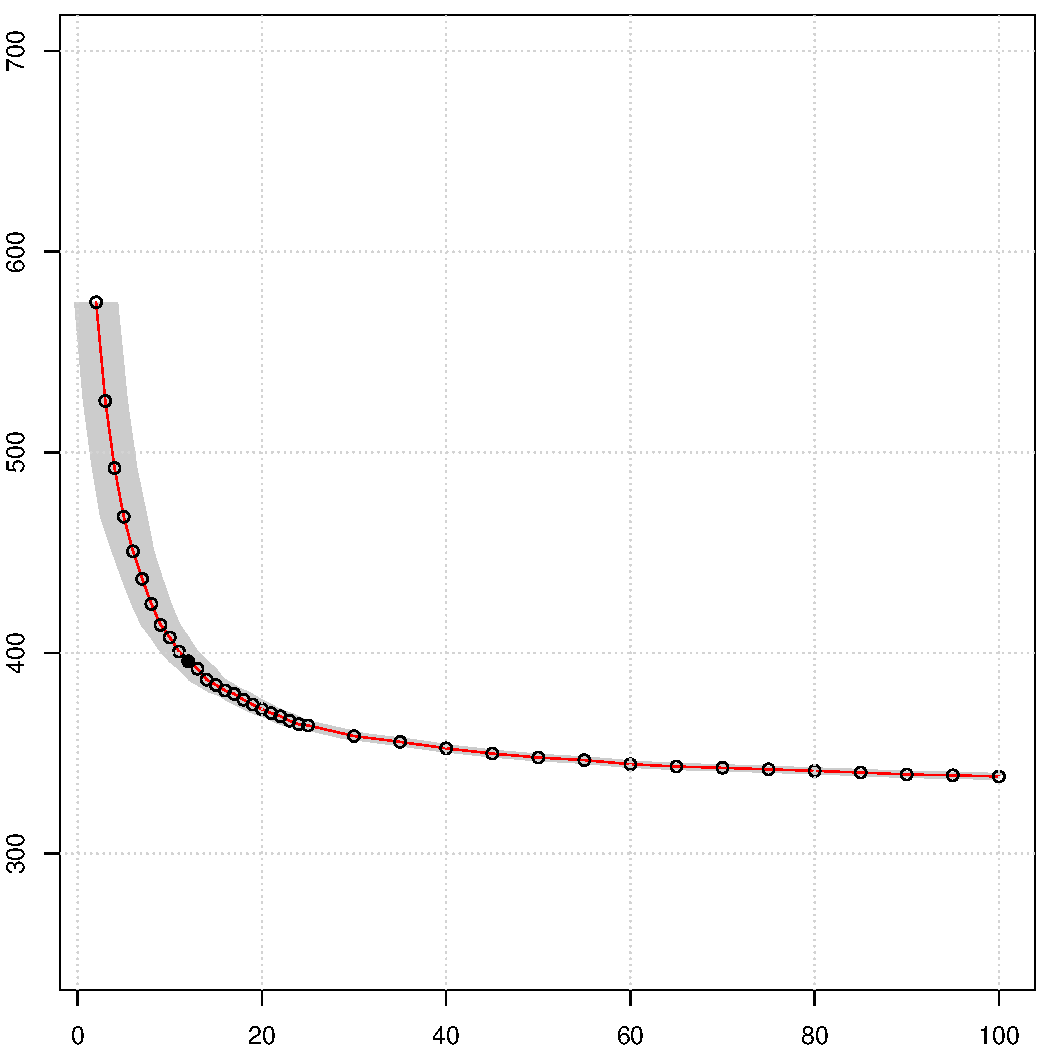
\includegraphics[width=7cm]{sensi-nu}
	}
%	\caption{$\text{ES}_{99\%}$ sensitivity to factor correlation and $\nu$}
	\caption{$\text{ES}_{99\%}$ sensitivity to copula parameters}
	\label{fig:sensi2}
\end{figure}

The main drawback of sensitivity analysis is that it measures the impact 
of the uncertainty of a parameter fixing the other ones. Another drawback 
is that it does not consider the distribution of the parameters. The 
section that follows provides a solution to these problems.

%------------------------------------------------------------------------------
% PARAMETERS UNCERTAINTY
%------------------------------------------------------------------------------
\section{Parameters Uncertainty}

The estimation of dependence parameters (degrees of freedom $\nu$, factor
loadings $\vec{w}$, and factor correlation matrix $R$) has an uncertainty 
that cannot be ignored~\cite{tarashev:2010,gossl:2005}. Example~\ref{ex:calib} 
illustrates this phenomenon and its magnitude (see the \emph{20 observations} 
case).

The CCruncher framework encourages incorporating the parameter uncertainty 
into the credit risk valuation. This indicates that credit risk measures
(e.g., $\text{VaR}_{99\%}$, $\text{ES}_{99\%}$) are regarded as distributions 
instead of values. For example, in the case of the Value at Risk, we consider
the function $\text{VaR}_{99\%}(L_T(\nu,\vec{w},R))$ that depends on 
the multivariate random variables $\nu, \vec{w}$ and $R$. Note that Expected 
Loss is not affected by the uncertainty of dependence parameters because the 
expectation satisfies $\text{E}(X+Y)=\text{E}(X)+\text{E}(Y)$ even if $X$ is 
not statistically independent of $Y$.

The solution recommended by CCruncher to determine the credit risk measure 
distribution is the obvious one and is based on the identical procedure 
used to determine the distribution of the portfolio loss or the distribution 
of the parameters: the random sampling of the risk measure distribution. 

On one hand, we have a procedure that generates random samples from the 
multivariate parameters distribution (see proposition~\ref{prop:pemh}).
These samples can be filtered to obtain a sample of independent parameters 
values.

On the other hand, we are able to measure the credit risk of a portfolio 
considering that dependence parameters are fixed values. This is performed 
sampling the portfolio loss (see algorithm~\ref{alg:pldmc}) and computing 
the credit risk measure using the appropriate statistic (see 
section~\ref{sec:riskm}).

We combine both components to define an algorithm that samples the desired
credit risk measure. The empirical density given by this sample 
approximates the risk measure distribution and allows evaluating the 
effect of the parameter uncertainty. One must be cautious because this 
procedure unveils the parameter uncertainty, but other uncertainties remain 
hidden such as:
\begin{inparaenum}[1)]
	\item copula selection, 
	\item factors/sectors selection and assignation,
	\item PDs uncertainty, and
	\item EAD and LGD models accuracy.
\end{inparaenum}

\begin{algorithm}[Credit risk measure distribution]
	\label{alg:crmd}
	Assume a portfolio (ratings, sectors, PDs, EADs, LGDs) and the number 
	of defaults observed by sector-rating in the previous years. We can
	determine the distribution of a credit risk measure 
	(e.g., $\text{VaR}_{99\%}$) by performing the following:
	\begin{enumerate}
		\item Obtain an ergodic sample of the parameters applying the
		Metropolis-Hastings algorithm (see proposition~\ref{prop:pemh}).
		\item Remove the first iterations (burn-in period), and determine
		the minimum common length $B$ at which the ACFs are $0$.
		\item Let $\{\nu^t, \vec{z}^t, R^t\}_{t=1,\dots,N}$ be the subsample
		of the parameters distribution composed by the indexes multiples 
		of $B$.
		\item For each simulated parameter, simulate the portfolio loss 
		distribution $L_T(\nu^t,\vec{w}^t,R^t)$ using the algorithm~\ref{alg:pldmc}.
		\item For each simulated portfolio loss distribution, compute its 
		risk measure using the statistic described in section~\ref{sec:riskm}:
		$\{\text{VaR}_{99\%}(L_T(\nu^t,\vec{w}^t,R^t))\}_{t=1,\dots,N}$.
	\end{enumerate}
\end{algorithm}

\begin{example}[Credit risk considering parameters uncertainty]
	\label{ex:paramu}
	We use the identical scenario as that described in example~\ref{ex:test05} 
	and that corresponds to CCruncher input file \texttt{test05.xml}. We 
	generate 20 observations of annual numbers of defaults using the 
	algorithm~\ref{alg:snod} (in the real world, these observations are extracted
	from the historical records). 
	In the following lines, we apply algorithm~\ref{alg:crmd} to estimate 
	the $\text{ES}_{99\%}$ distribution, considering the parameters' 
	uncertainty. 

	The first step includes the generation of a sample of the parameters' 
	distribution using the Metropolis-Hastings algorithm. We performed 
	\num{1000000} iterations. Figure~\ref{fig:paramu1} displays the 
	marginals of this distribution.
	
	The second step is removing the first \num{20000} iterations (burn-in 
	period) and determining the thin interval using the ACFs. 
	Figure~\ref{fig:paramu2} shows the ACF for each parameter. A thin interval 
	of \num{3000} is sufficient in this example. 
	
	The third step is pruning the parameters sample preserving 
	only the simulated values whose index is a multiple of \num{3000}. 
	Below is displayed part of the simulated values:

	\hspace*{1cm}
	\begin{tabular}{cc|c|c|c|c|}
		\cline{1-1} \cline{3-6}
		\multicolumn{1}{|c|}{N} & & $\nu$ & $w_1$ & $w_2$ & $R_{12}$ \\
		\cline{1-1} \cline{3-6}
		\multicolumn{1}{|c|}{1} & & 12.54 & 0.29 & 0.48 & 0.21 \\
		\cline{1-1} \cline{3-6}
		\multicolumn{1}{|c|}{2} & & 10.77 & 0.28 & 0.32 & -0.28 \\
		\cline{1-1} \cline{3-6}
		\multicolumn{1}{|c|}{\vdots} & & \vdots & \vdots & \vdots & \vdots \\
		\cline{1-1} \cline{3-6}
		\multicolumn{1}{|c|}{300} & & 10.06 & 0.33 & 0.36 & 0.02 \\
		\cline{1-1} \cline{3-6}
	\end{tabular}

	The fourth step is the simulation of the portfolio loss distribution
	for each simulated parameter. This is quite an intensive computation.
	The CCruncher's command line execution and the input file macro expansion
	can assist in performing this step. Listing~\ref{sc:paramu4} displays a 
	simple batch script to sequentially execute the required simulations.
	Those who have a cluster, a cloud or a grid may consider to executing 
	multiple parallel tasks using a framework such as MakeFlow\footnotemark[1]
	or something similar. 

	Finally, the fifth step is the computation of the risk statistic
	for each portfolio loss distribution. The density of the $\text{ES}_{99\%}$ 
	can be approximated using the empirical density. Listing~\ref{sc:paramu5}
	provides an R script to perform this task. 

	The exact value of the $\text{ES}_{99\%}$ assuming that parameters are 
	fixed and known is $\approx 383$\ \euro\ (see example~\ref{ex:test05}). 
	If we do not assume that parameters are known and we infer the parameters 
	from 20 observations of the numbers of defaults, then we obtain the 
	distribution displayed in figure~\ref{fig:paramu5}. 
	The key point is to dispose a distribution indicating the 
	feasible values that can take the risk measure $\text{ES}_{99\%}$.
\end{example}
\footnotetext[1]{\url{http://www3.nd.edu/~ccl/software/makeflow/}} 
\begin{comment}
# R script to simulate values
source("/home/gerard/projects/ccbinf/bin/ccbinf.R")
p = c(0.05, 0.1, 0.2)
w = c(0.4, 0.35)
D = matrix(nrow=2, ncol=3, data=c(167, 167, 166, 167, 167, 166))
R = matrix(ncol=2, nrow=2, data=c(1.0,0.25,0.25,1.0))
nu = 15
rcount = ccruncher.rcount(20, p, D, w, R, nu)
export(rcount, "paramu.txt")

# bash commands
/home/gerard/projects/ccbinf/build/ccbinf -r 1000 -n 1000000 paramu.txt
\end{comment}

\begin{figure}[!ht]
	\centering
	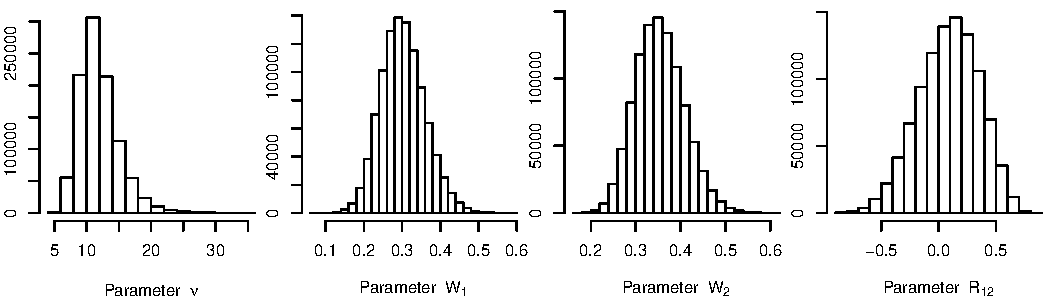
\includegraphics[width=0.98\textwidth]{paramu-1}
	\caption{Step 1 -- Parameters sampling using M-H}
	\label{fig:paramu1}
\end{figure}

\begin{figure}[ht]
	\centering
	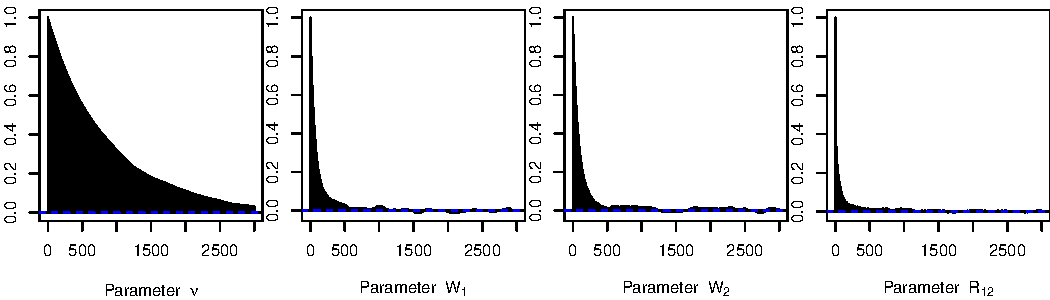
\includegraphics[width=0.98\textwidth]{paramu-2}
	\caption{Step 2 -- ACF of simulated parameters}
	\label{fig:paramu2}
\end{figure}

\begin{lstlisting}[language=bash, label={sc:paramu4}, caption={Execution of multiple CCrunchers (bash script)}]
 
 mkdir data/MH001;
 bin/ccruncher-cmd -o data/MH001 -DNU=12.54 -DW1=0.29 \
     -DW2=0.48 -DR12=0.21 samples/test05.xml > data/MH001/ccruncher.out; 
 
 mkdir data/MH002; 
 bin/ccruncher-cmd -o data/MH002 -DNU=10.77 -DW1=0.28 \
     -DW2=0.32 -DR12=-0.28 samples/test05.xml > data/MH002/ccruncher.out;

 ...

 mkdir data/MH300; 
 bin/ccruncher-cmd -o data/MH300 -DNU=10.06 -DW1=0.33 \
     -DW2=0.36 -DR12=0.02 samples/test05.xml > data/MH300/ccruncher.out; 
 
\end{lstlisting}

\begin{lstlisting}[language=R, label={sc:paramu5}, caption={$ES_{99\%}$ distribution (R script)}]

 getRisk <- function(dir)
 {
   filename = paste(dir, "/portfolio.csv", sep="")
   data <- read.csv(filename, comment.char="#")
   X = sort(data[,1])
   n = length(X)
   Y = X[as.integer(n*0.99):n]
   ES99 = mean(Y)
   sde = sqrt(var(Y)/length(Y))
   return(c(ES99,sde))
 }

 dirs = dir("data", pattern="MH[[:digit:]{3}]*", full.names=TRUE)
 values = matrix(ncol=2,nrow=length(dirs))
 colnames(values) = c("ES99", "stderr")
 for(i in 1:length(dirs)) {
   values[i,] = getRisk(dirs[i])
 }
 
 plot(density(values[,1]))
 
\end{lstlisting}

\begin{figure}[!ht]
	\centering
	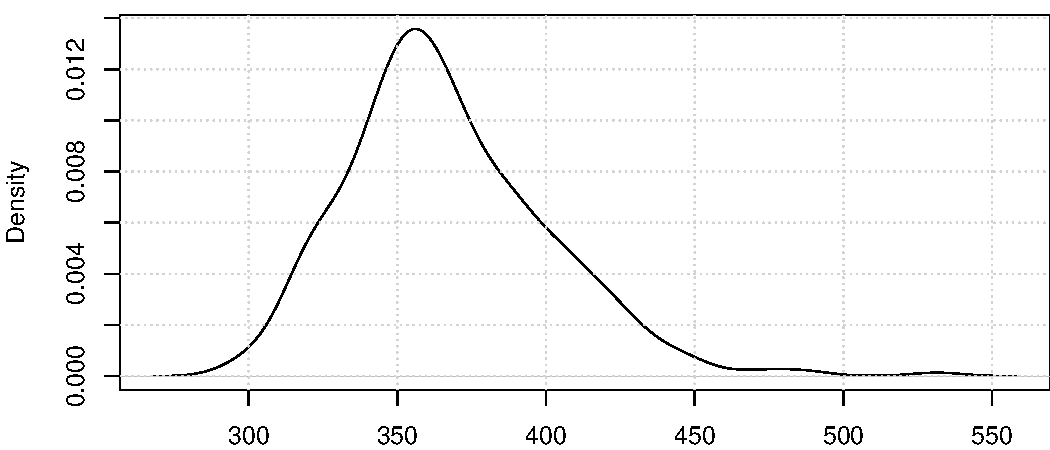
\includegraphics[width=0.98\textwidth]{paramu-5}
	\caption{$\text{ES}_{99\%}$ distribution}
	\label{fig:paramu5}
\end{figure}

%------------------------------------------------------------------------------
% PORTFOLIO OPTIMIZATION
%------------------------------------------------------------------------------
\section{Portfolio Optimization}

Once we knows the portfolio credit risk, naturally arises the question ``How 
can I balance the weights assigned to each business unit so that the total 
portfolio risk is minimized?'' In section \ref{ss:ra}, we have seen that 
CCruncher allows defining sub-portfolios and it can disaggregate the portfolio 
credit risk in terms of them. In this section we will see how to modify the 
weights assigned to each sub-portfolio in order to optimize the portfolio
credit risk. First of all, let's define the problems considered:

\begin{definition}[Portfolio optimization]
	Let a portfolio composed of $K$ sub-portfolios. We want to determine the 
	sub-portfolio weights $\alpha_k$ that minimize one of the following 
	problems\footnotemark[2].

	{\centering
	\renewcommand{\arraystretch}{1.5}
	\begin{tabular}{l m{1cm} l m{1cm} l}
		\textbf{EL minimization} & & \textbf{ES minimization} & & \textbf{EL-ES minimization} 
		\\
		$\displaystyle \min_{\alpha_k} \ \text{EL}(L)$
		& &
		$\displaystyle \min_{\alpha_k} \ \text{ES}_{99\%}(L)$
		& &
		$\displaystyle \min_{\alpha_k} \ \sqrt{\text{EL}^2+\text{ES}_{99\%}^2}$
		\\
		Subjecto to:
		& &
		Subjecto to:
		& &
		Subjecto to:
		\\
		$\left.
			\begin{array}{l}
				x^0 = \text{ES}_{99\%}(L) \\
				0 \le \alpha_k \le 1 \quad \forall k \\
				\displaystyle \sum_{k=1}^{K} \alpha_k = 1 \\
			\end{array}
			\right\}
		$
		& &
		$\left.
			\begin{array}{l}
				y^0 = \text{EL}(L) \\
				0 \le \alpha_k \le 1 \quad \forall k \\
				\displaystyle \sum_{k=1}^{K} \alpha_k = 1 \\
			\end{array}
			\right\}
		$
		& &
		$\left.
			\begin{array}{l}
				\\
				0 \le \alpha_k \le 1 \quad \forall k \\
				\displaystyle \sum_{k=1}^{K} \alpha_k = 1 \\
			\end{array}
			\right\}
		$
	\end{tabular}\par}
	where $L=L_1+\dots+L_k$ is the portfolio loss, and $x^0$ and $y^0$ are 
	fixed values.
\end{definition}

\footnotetext[2]{We use $\text{ES}_{99\%}$ but you can use any other risk 
measure depending on copula parameters, such as $\text{ES}_{95\%}$ or 
$\text{VaR}_{99\%}$.}

Sub-portfolio weights $\alpha_k$ are the sub-portfolio exposures relative 
to total portfolio exposure at 1-year. The way to balance the portfolio 
composition is to add or subtract obligors preserving the characteristics 
of each sub-portfolio. When we try to model this procedure we find two 
problems:
\begin{inparaenum}[1)]
	\item losses of portfolios with distinct composition are not comparable, 
	\item it is unclear the procedure to modify the composition of a 
		sub-portfolio (we add half a debtor?, to wich rating and sector we 
		assign the new obligor?, new obligors have an averaged exposure and 
		recovery?).
\end{inparaenum}

Fortunately these two problems are solvable. The first one is avoided
considering the relative losses on exposure rather than absolute losses. 
Thus, the relative portfolio loss at time horizon $T$ is
\begin{displaymath}
	L_T = \frac{
	\displaystyle \sum_{i=1}^n \mathbbm{1}_{[0,T]}(t_i) \cdot 
	\left( 
	\sum_{j=1}^{m_i} \text{EAD}_i^j(t_i) \cdot \text{LGD}_i^j(t_i)
	\right)}
	{\displaystyle \sum_{i=1}^n
	\left( 
	\sum_{j=1}^{m_i}\ \underset{[0,T]}{\text{avg}} \left( \text{EAD}_i^j(t) \right)
	\right)}
\end{displaymath}
where $T$ is the time horizon where portfolio loss is computed, $n$ is the 
number of obligors, $(t_1,\dots,t_n)$ are the obligors' default times, $m_i$ 
is the number of assets of the i-th obligor, and $\text{EAD}_i^j(t)$ and 
$\text{LGD}_i^j(t)$ are the EAD and LGD functions of the j-th asset of the 
i-th obligor evaluated at time $t$.

The second problem, the portfolio composition, is avoided by equating the number 
of obligors to exposures. Suppose we have two sub-portfolios A and B with the 
same exposure, the first one with 500 obligors, and the second one with 500 
obligors. We want to balance the portfolio so that ends up with $25\%$ of the 
exposure in A and $75\%$ in B. The way to implement it is eliminating 
half of the obligors from A and adding $250$ new obligors similar to those of 
B. That said, if sub-portfolios A and B have a large number of homogeneous 
individuals, then we can maintain the original number of individuals 
($500+500$) and balance the portfolio by multiplying by $0.5$ the A's exposures 
and by $1.5$ the B's exposures.

\begin{figure}[!ht]
	\centering
	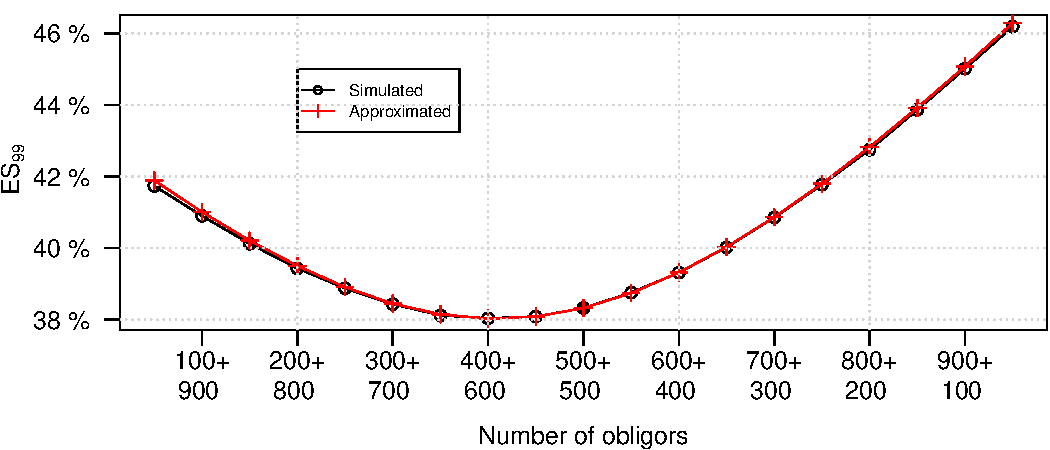
\includegraphics[width=0.98\textwidth]{sensi-pct}
	\caption{$\text{ES}_{99\%}$ for distinct percentages of S1 and S2}
	\label{fig:popt2}
\end{figure}

\begin{example}[Sub-portfolio weights]
	To check the accuracy of the equivalence between the number of individuals 
	and the exposures we analyze the case \texttt{test05.xml} (see 
	example~\ref{ex:test05}) considering the sub-portfolios S1 ( = S1A + 
	S1B + S1C) and S2 (= S2A + S2B + S2C). In this example we consider only two 
	sub-portfolios, rather than the six defined, so that the values can be 
	clearly represented in the plane. First, we simulate different portfolio 
	compositions (50+950, 100+900, \dots, 950+50) and calculate the 
	$\text{ES}_{99\%}$ for each of them. Next, we consider a fixed number of 
	individuals (500+500) and we change the exposure of individuals according to 
	its sector so that we mimic the previous compositions. Figure \ref{fig:popt2} 
	displays the values modifying the composition of the portfolio (simulated) 
	and the values modifying the exposure of the obligors (approximated). In this 
	case, both values are similar, with an error less than $0.15\%$.
\end{example}

The equivalence between the number of debtors and the exposures has a very 
important advantage since it allows optimizing without having to do multiple 
simulations. This is achieved by simulating the losses of the current portfolio
and by reusing these values to calculate any desired composition of the 
portfolio. The following algorithm computes the risk of a weighted portfolio 
reusing the simulated losses from the current portfolio.

\begin{algorithm}[Risk of a weighted portfolio]
	\label{alg:rwp}
	Let a portfolio composed of $K$ sub-portfolios with an average exposure $E_k$ 
	for each of them in the period $[0, T]$. We have simulated the portfolio 
	losses broken down by sub-portfolios. We want compute the EL and 
	$\text{ES}_{99\%}$ of this portfolio with weights $\alpha_1,\dots,\alpha_K$.
	\begin{enumerate}
		\item Obtain multiplicative factors: 
		$\lambda_k = \alpha_k \cdot \frac{E}{E_k} = \frac{\alpha_k}{\alpha_k^0}$
		\item Create weighted losses: $y_i = \displaystyle \sum_{k=1}^K \lambda_k \cdot x_i^k \quad i=1,\dots,N$
		\item Compute EL (see section~\ref{sec:riskm}) using values $\left\{y_i\right\}_{i=1,\dots,N}$ 
		and divide this value by $E$ to obtain the EL relative to total exposure.
		\item Compute $\text{ES}_{99\%}$ (see section~\ref{sec:riskm}) using values 
		$\left\{y_i\right\}_{i=1,\dots,N}$ and divide this value by $E$ to obtain the 
		$\text{ES}_{99\%}$ relative to total exposure.
	\end{enumerate}
	where $E = \sum_{k=1}^K E_k$ is the total exposure, $\alpha_k^0$ is the weight
	of the current k-th sub-portfolio, $N$ is the number of simulated losses, and
	$x_i^k$ is the i-th simulated loss of the k-th sub-portfolio.
\end{algorithm}

The risk of weighted portfolio is continuous with respect to $\alpha_1,\dots,\alpha_K$
but it is not linear with respect to this parameters because the rank statistic 
involved in the $\text{VaR}_{99\%}$ and $\text{ES}_{99\%}$ measures. 
This is illustrated in figure~\ref{fig:popt2}.

\begin{example}[Feasible portfolios]
	We consider the portfolio defined in \texttt{test05.xml} (see example~\ref{ex:test05}).
	We want to know the values that can take the risk measures by changing the 
	composition of the portfolio. To achieve this, we consider the following 
	weights:
	\begin{displaymath}
		\left\{
		\left( \alpha_1,\dots,\alpha_6 \right) \mid
		\alpha_i \in \left\{0, 0.1, 0.2,\dots,0.9,1 \right\}
		\ \text{ and }\ \displaystyle \sum_{i=1}^6 \alpha_i = 1
		\right\}
	\end{displaymath}
	This set of weights has \num{3003} elements. For each element of this set we
	compute the EL and $\text{ES}_{99\%}$ of the weighted portfolio applying the
	algorithm~\ref{alg:rwp}. Result is displayed in figure~\ref{fig:optim1}. We
	have drawn the convex hull of the region and we have identified the relevant 
	points. The original portfolio is marked with a black dot and the 
	corresponding optimal portfolios are indicated with a arrow. The appearance 
	of the EL-ES region is determined by the involved sub-portfolios, in this 
	case: S1A, S1B, S1C, S2A, S2B, S2C. Other segmentations (e.g., geographic 
	areas, types of products) will lead to EL-ES regions with a different shape. 
\end{example}

\begin{figure}[!ht]
	\centering
	\subcaptionbox{Portfolio values}{
		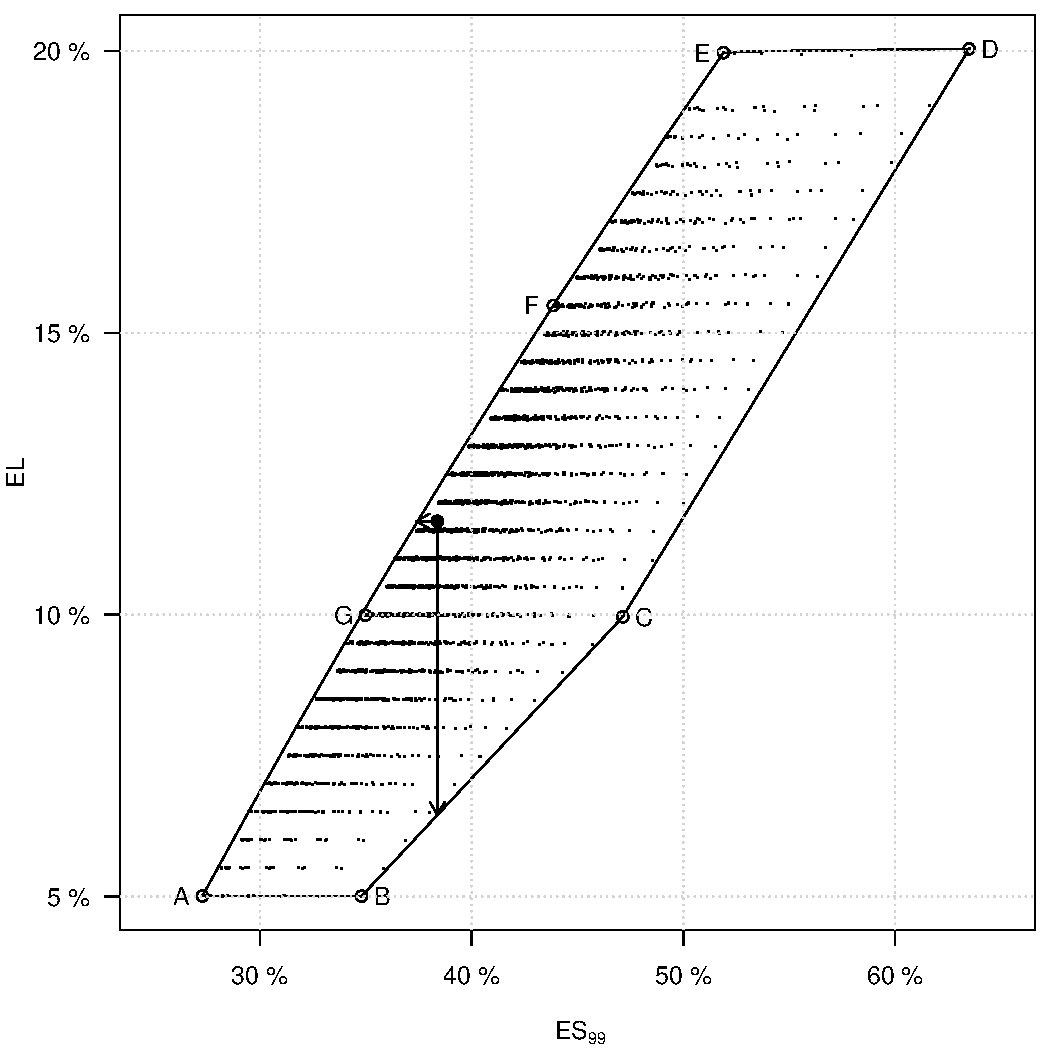
\includegraphics[width=6.5cm]{optim1}
	}
	\subcaptionbox{Portfolio composition}{
		\small
	    \begin{tabular}{c|rrrrrr}
			  & S1A   & S1B   & S1C   & S2A   & S2B & S2C   \\
			\hline
			A &  40\% &   0\% &   0\% &  60\% & 0\% &   0\% \\
			B & 100\% &   0\% &   0\% &   0\% & 0\% &   0\% \\
			C &   0\% & 100\% &   0\% &   0\% & 0\% &   0\% \\
			D &   0\% &   0\% & 100\% &   0\% & 0\% &   0\% \\
			E &   0\% &   0\% &  40\% &   0\% & 0\% &  60\% \\
			F &  10\% &   0\% &  30\% &  20\% & 0\% &  40\% \\
			G &  20\% &  10\% &  10\% &  40\% & 0\% &  20\% \\
		\end{tabular}
		\vspace{50pt}
	}
	\caption{\texttt{test05.xml} feasible portfolios}
	\label{fig:optim1}
\end{figure}

Now we have all the elements to solve the three optimization problems. Instead
of presenting the algorithm in pseudo-code, this time we use a basic R script 
exposed in listing~\ref{sc:opt} to illustrate the procedure. The optimized 
portfolio is the case \texttt{test05.xml} and optimization results are listed
in table~\ref{tab:optim1}. Note that $K-1$ parameters are optimized rather 
than $K$. This is because we can obtain the former doing 
$\alpha_1 = 1-\sum_{i=2}^K \alpha_i$. Note also that penalty functions are 
used to ensure the restrictions compliance.

\begin{lstlisting}[language=R, label=sc:opt, caption=Portfolio optimization (R script)]

 evalPortfolio <- function(losses, w0, w1, level=0.99)
 {
   if (length(w0) != length(w1)) stop("invalid parameters")
   if (ncol(losses) != length(w0)) stop("invalid losses")
   if (level <= 0 || level >= 1) stop("ES level out-of-range (0,1)")
   n = nrow(losses)
   k = ncol(losses)
   lambda = w1/w0
   loss = rep(0, n)
   for(i in 1:k) {
     loss = loss + losses[,i]*lambda[i]
   }
   loss = sort(loss)
   el = mean(loss)
   es = mean(loss[as.integer(n*level):n])
   return(c(el,es))
 }

 getW <- function(params)
 {
   w = c(0, params)
   w[1] = 1-sum(w)
   return(w)
 }

 f <- function(params, losses, w0, option, val, level=0.99)
 {
   if (!(option %in% (1:3))) stop("unrecognized option")
   w1 = getW(params)
   aux = 0
   if (w1[1] < 0) {
     aux = w1[1]
     w1[1] = 0
   }
   eles = evalPortfolio(losses, w0, w1, level)
   if (aux != 0) {
     eles = eles + abs(aux)*10
   }
   if (option == 1) {
     ret = eles[1] + 10*(val-eles[2])^2
     return(ret)
   }
   else if (option == 2) {
     ret = eles[2] + 10*(val-eles[1])^2
     return(ret)
   }
   else if (option == 3) {
     ret = sqrt(sum(eles^2))
     return(ret)
   }
   else return(NA)
 }

 losses <- read.csv("data/sector-rating.csv", comment.char="#")
 exposures = c(167, 166, 167, 167, 167, 166)
 w0 = exposures/sum(exposures)
 eles0 = evalPortfolio(losses, w0, w0)
 
 # EL minimization
 params = w0[2:length(w0)]
 opt = nlminb(params, f, losses=losses, w0=w0, option=1, val=eles0[2],
       lower=rep(0,length(params)), upper=rep(1,length(params)))
 w1 = getW(opt$par)
 evalPortfolio(losses, w0, w1)

 # ES minimization
 params = w0[2:length(w0)]
 opt = nlminb(params, f, losses=losses, w0=w0, option=2, val=eles0[1],
       lower=rep(0,length(params)), upper=rep(1,length(params)))
 w2 = getW(opt$par)
 evalPortfolio(losses, w0, w2)

 # optimization
 params = w0[2:length(w0)]
 opt = nlminb(params, f, losses=losses, w0=w0, option=3, val=NA,
       lower=rep(0,length(params)), upper=rep(1,length(params)))
 w3 = getW(opt$par)
 evalPortfolio(losses, w0, w3)
 
\end{lstlisting}

\begin{table}[!hb]
\begin{tabular}{l|rrrrrr|rr}
	          & S1A   & S1B   & S1C   & S2A   & S2B   & S2C   & EL    & ES \\
	\hline
	current   &16.7\% &16.6\% &16.7\% &16.7\% &16.7\% &16.6\% &11.6\% &38.3\% \\
	min EL    &68.9\% &31.1\% &   0\% &   0\% &   0\% &   0\% & 6.6\% &38.3\% \\
	min ES    &18.7\% &   0\% &21.3\% &36.8\% &   0\% &23.2\% &11.6\% &37.2\% \\
	min EL-ES &41.0\% &   0\% &   0\% &59.0\% &   0\% &   0\% & 5.0\% &27.0\% \\
\end{tabular}
	\caption{\texttt{test05.xml} optimization}
	\label{tab:optim1}
\end{table}


%==============================================================================
% APPENDICES
%==============================================================================
\appendix
\chapter{Appendices}

%------------------------------------------------------------------------------
% THE PROBABILITIES OF DEFAULT
%------------------------------------------------------------------------------
\section{The Probabilities of Default}
\label{ap:pd}

In this section, we construct the univariate time-until-default obligor 
distributions using available information such as the 1-year PDs or the ratings
transition matrix. The objective is to determine the cumulative density 
functions $F_i(t) = \Pr\{T_i \le t\}$ for each of the ratings.

\begin{definition}[Probability of Default (PD)]
	$T_i$ is the random variable that represents the default time 
	(aka time-until-default, aka survival time, aka time-to-default) of the 
	i-th obligor. Let $F_i(t)$ denote the distribution function of $T_i$:
	\begin{displaymath}
		F_i(t) = \Pr\{T_i \le t\} = 
		\Pr\{\text{ i-th obligor defaults before $t$ years }\}
	\end{displaymath}
	Note that $F_i(t)$ is the probability of default (PD) of the i-th obligor
	at time horizon $t$. PD is a key parameter used in the calculation of credit 
	risk under Basel II\@. We indicate as $p_i$ the probability that i-th obligor 
	defaults within the time range $[0,1]$.
	\begin{displaymath}
		p_i = \Pr\{T_i \le 1\ \text{year}\} = F_i(1) 
	\end{displaymath}
\end{definition}

Each obligor has its own time-until-default distribution depending on its 
rating; therefore, all obligors with identical ratings have identical
distributions. Below, we indicate three different manners of inferring $F_i$ 
depending upon the amount of information available. All three manners produce 
similar results in the short term (e.g., 1 year) but differ in the middle and
long term. Before detailing the different approaches, we define the transition 
matrix because it is used in all three cases.

\begin{definition}[Transition matrix]
	\label{def:tm}
	The $T$-years transition matrix gives the probability of changing 
	from i-th rating to j-th rating in a period of $T$ years:
	{\small
	\begin{displaymath}
		M_T = \left(
		\begin{array}{ccc}
			m_{11} & \cdots & m_{1r} \\
			\vdots & \ddots & \vdots \\
			m_{r1} & \cdots & m_{rr} \\
		\end{array}
		\right)
	\end{displaymath}\par}
	in which $r$ is the number of ratings and $m_{ij}$ is the probability that 
	an obligor with i-th rating ends up having the j-th rating after $T$ years.
	Note that row sums are $1$ and that two consecutive transition matrices, 
	$M_{T_1}$ and $M_{T_2}$, give $M_{T_1+T_2} = M_{T_1} \cdot M_{T_2}$.
	A valid transition matrix must have a unique \emph{defaulted} rating, and 
	any rating ends up defaulting.
\end{definition}

\begin{example}[1-year transition matrix]
	\label{ex:1ytm}
	Table~\ref{tmatrix1} shows a transition matrix, extracted 
	from~\cite[p. 20]{cmetrics:1997}, in which the probability that an obligor 
	with rating AA changes to rating B in one year is $0.14\%$. Note that the
	last column contains the 1-year default probabilities for each rating and 
	that the last row corresponds to the \emph{defaulted} rating.
\end{example}

\begin{table}[!ht]
	\begin{center}
		\begin{tabular}[]{l|rrrrrrrr}
							& AAA     & AA      & A       & BBB     & BB      & B                  & CCC     & Default  \\
			\hline
			AAA     & $90.81$ & $8.33$  & $0.68$  & $0.06$  & $0.12$  & $0.00$             & $0.00$  & $0.00$   \\
			AA      & $0.70$  & $90.65$ & $7.79$  & $0.64$  & $0.06$  & $\underline{0.14}$ & $0.02$  & $0.00$   \\
			A       & $0.09$  & $2.27$  & $91.05$ & $5.52$  & $0.74$  & $0.26$             & $0.01$  & $0.06$   \\
			BBB     & $0.02$  & $0.33$  & $5.95$  & $86.93$ & $5.30$  & $1.17$             & $0.12$  & $0.18$   \\
			BB      & $0.03$  & $0.14$  & $0.67$  & $7.73$  & $80.53$ & $8.84$             & $1.00$  & $1.06$   \\
			B       & $0.00$  & $0.11$  & $0.24$  & $0.43$  & $6.48$  & $83.46$            & $4.07$  & $5.21$   \\
			CCC     & $0.22$  & $0.00$  & $0.22$  & $1.30$  & $2.38$  & $11.24$            & $64.86$ & $19.78$  \\
			Default & $0.00$  & $0.00$  & $0.00$  & $0.00$  & $0.00$  & $0.00$             & $0.00$  & $100.00$ \\
		\end{tabular}
		\caption{1-year transition matrix \%}
		\label{tmatrix1}
	\end{center}
\end{table}

\subsection{Obtaining PDs from the transition matrix}
\label{pdftm}

This alternative implies that transition probabilities remain constant
over time, undermining the economic cycle effect. In practice, this constancy
is equivalent to considering an averaged economic cycle. 
See document~\cite[sec. 3.2.1]{bindseil:2007} to obtain additional information
related with this section and the CreditMetrics\texttrademark{} approach.

\begin{proposition}[Scaled transition matrix]
	The transition matrix can be scaled in time using the following rules:
	\begin{itemize}
		\item $M_{k \cdot T} = M_{T}^k$
		\item $M_{\frac{T}{k}} = \sqrt[k]{M_{T}}$
	\end{itemize}
\end{proposition}

The root of a matrix $M$ can be obtained using the spectral decomposition
$M = P \cdot D \cdot P^{-1}$ doing $M^{k} = P \cdot D^{k} \cdot P^{-1}$, 
in which $P$ and $D$ are the eigenvectors and eigenvalue matrices of $M$. 

Sometimes, the scaled transition matrix does not satisfy the Markov conditions
(the row sum is equal to one, and all elements are non-negatives). In this case, 
we must transform this matrix to the relevant Markov matrix. This process is 
called regularization. Below is the QOM regularization algorithm extracted 
from~\cite{kreinin:2001}.

\begin{algorithm}[Transition matrix regularization]
	The QOM (Quasi-Optimization of the root Matrix) algorithm regularizes an 
	$n {\times} n$ transition matrix $M$, row by row. The steps to 
	regularizing the $i$-th row are
	\begin{enumerate}
		\item Compute the difference between the row sum and one. 
		Divide by $n$ and subtract this value from all non-zero components:
		\begin{displaymath}
			m_{ij} \ne 0 
			\Longrightarrow 
			m_{ij} = m_{ij} - \frac{1}{n} \left( \sum_{k=1}^{n} m_{ik} - 1\right)
		\end{displaymath}
		\item If all the row elements are non-negative and add up to one, 
		then stop: the row is regularized.
		\item Adjust any negative row element to zero and go to Step 1.
	\end{enumerate}
	The algorithm stops after $m$ steps, where $m \le n$. 
	Apply the previous algorithm to every row.
	The final matrix is a regularized matrix. 
\end{algorithm}

\begin{proposition}[PDs derived from transition matrix]
	\label{prop:pdftm}
	If $M_T$ is a transition matrix, then the time-until-default distribution 
	for an obligor with the i-th rating is
	\begin{displaymath}
		F_i(t) = \Pr\{T_. \le t\} = \left( M_t \right)_{id}
	\end{displaymath}
	in which $T_.$ is the time-until-default of an obligor with the i-th rating, 
	$d$ is the index of the \emph{defaulted} rating, $M_t$ is the transition 
	matrix scaled to time $t$, and $(M)_{ij}$ is the matrix element located in 
	the i-th row and the j-th column.
\end{proposition}

\begin{example}
	\label{ex:pdftm}
	We derive the time-until-default distribution for each rating induced by the 
	transition matrix presented in table~\ref{tmatrix1}. As a first step, we 
	scale the 1-year transition matrix $M_1$ to the 1-month transition matrix 
	$M_{\frac{1}{12}}$.
	{\small
	\begin{displaymath}
		M_{\frac{1}{12}} = \left(
		\begin{array}{cccccccc}
			99.1972 &  0.7588 &  0.0320 &  0.0020 &  0.0112 & -0.0011 & -0.0001 &   0.0000 \\
			 0.0635 & 99.1744 &  0.7083 &  0.0392 &  0.0015 &  0.0120 &  0.0018 &  -0.0007 \\
			 0.0074 &  0.2057 & 99.1980 &  0.5102 &  0.0557 &  0.0189 & -0.0001 &   0.0042 \\
			 0.0014 &  0.0239 &  0.5507 & 98.8021 &  0.5164 &  0.0871 &  0.0077 &   0.0106 \\
			 0.0027 &  0.0113 &  0.0396 &  0.7581 & 98.1557 &  0.8774 &  0.0889 &   0.0665 \\
			-0.0007 &  0.0098 &  0.0196 &  0.0111 &  0.6447 & 98.4443 &  0.4463 &   0.4240 \\
			 0.0233 & -0.0023 &  0.0170 &  0.1287 &  0.2166 &  1.2298 & 96.4213 &   1.9667 \\
			 0.0000 &  0.0000 &  0.0000 &  0.0000 &  0.0000 &  0.0000 &  0.0000 & 100 \\
		\end{array}
		\right)
	\end{displaymath}\par}
	We observe that $M_{\frac{1}{12}}$ is not a regular matrix because of 
	negative values. We apply the QOM algorithm to regularize it.
	{\small
	\begin{displaymath}
		\bar{M}_{\frac{1}{12}} = \left(
		\begin{array}{cccccccc}
			99.1969 &  0.7586 &  0.0317 &  0.0018 &  0.0110 &  0.0000 &  0.0000 &   0.0000 \\
			 0.0634 & 99.1744 &  0.7082 &  0.0391 &  0.0014 &  0.0119 &  0.0017 &   0.0000 \\
			 0.0074 &  0.2057 & 99.1980 &  0.5102 &  0.0557 &  0.0189 &  0.0000 &   0.0041 \\
			 0.0014 &  0.0239 &  0.5507 & 98.8021 &  0.5164 &  0.0871 &  0.0077 &   0.0106 \\
			 0.0027 &  0.0112 &  0.0395 &  0.7581 & 98.1557 &  0.8774 &  0.0889 &   0.0665 \\
			 0.0000 &  0.0099 &  0.0197 &  0.0111 &  0.6447 & 98.4444 &  0.4463 &   0.4240 \\
			 0.0228 &  0.0000 &  0.0165 &  0.1282 &  0.2161 &  1.2293 & 96.4208 &   1.9663 \\
			 0.0000 &  0.0000 &  0.0000 &  0.0000 &  0.0000 &  0.0000 &  0.0000 & 100 \\
		\end{array}
		\right)
	\end{displaymath}\par}
	We call the 1-year regularized transition matrix to 
	$\bar{M}_1 = \bar{M}_{\frac{1}{12}}^{12}$. 
	Finally, we use proposition~\ref{prop:pdftm} to determine the 
	PD function for each rating and month. The results are displayed in 
	figure~\ref{fig:pdftm}.
\end{example}

\begin{figure}[!ht]
	\centering
	\subcaptionbox{Probability of Default (100 years)}{
		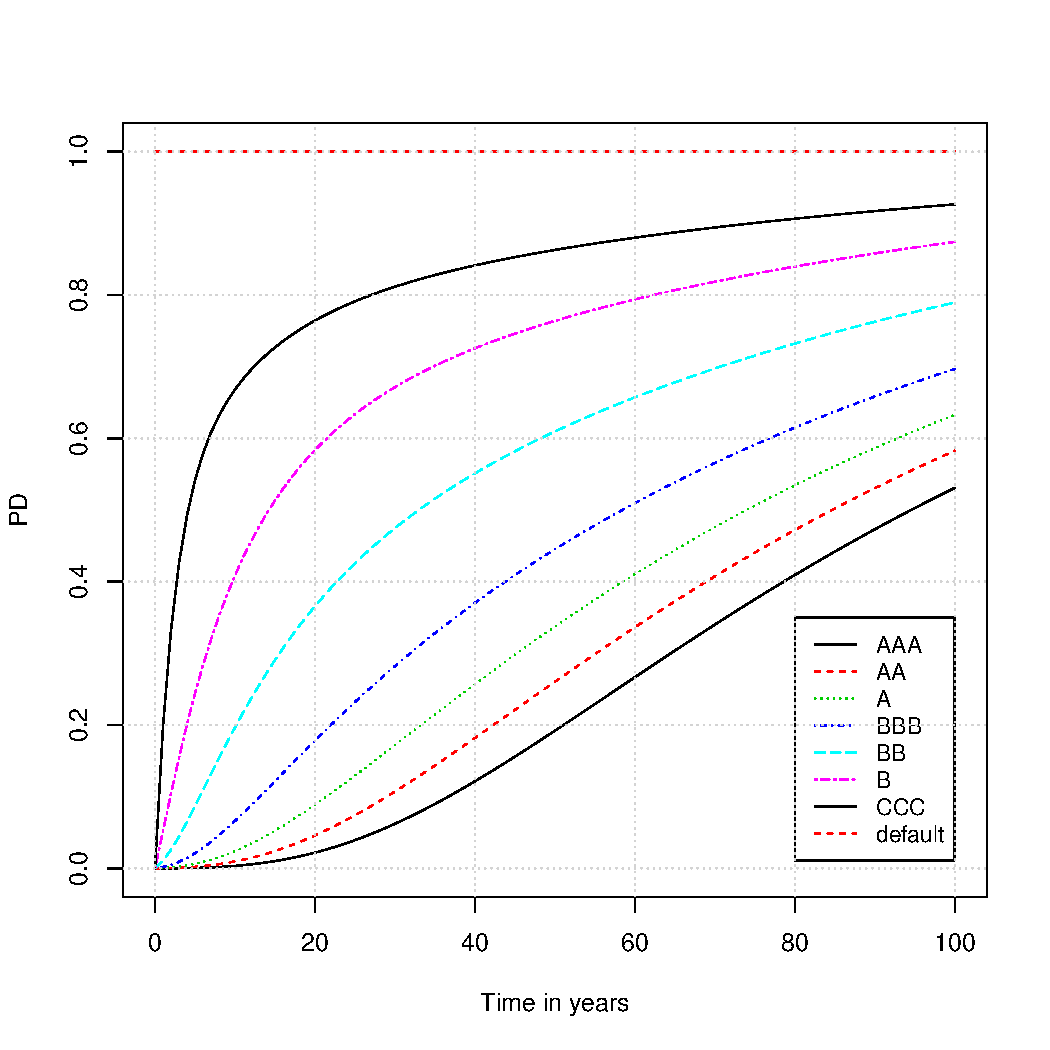
\includegraphics[width=7cm]{pdftm1}
	}
	\subcaptionbox{Probability of Default (10-year zoom)}{
		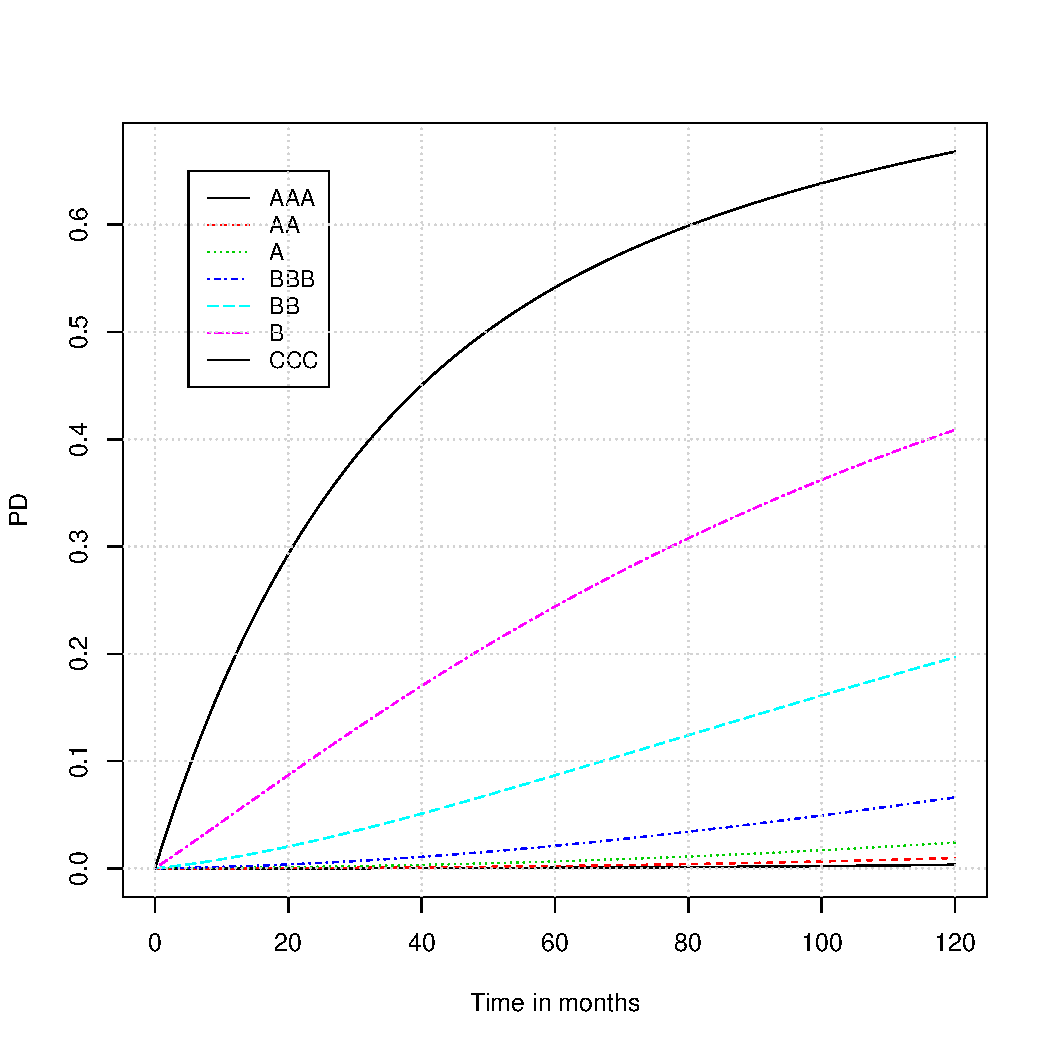
\includegraphics[width=7cm]{pdftm2}
	}
	\caption{PDs derived from transition matrix}
	\label{fig:pdftm}
\end{figure}

\subsection{Obtaining PDs from annual values}
\label{pdfsv}

In some circumstances, the transition matrix is not available, and we only 
have the probability of default at 1-year for each rating, 
$p_1,\dots,p_{r-1},p_r$ in which the r-th rating is the \emph{defaulted} 
status. In the absence of more information, we can consider a diagonal 
transition matrix such as the following:
\begin{displaymath}
	M_1 = \left(
	\begin{array}{cccc}
		1-p_1  & \cdots & 0         & p_1     \\
		\vdots & \ddots & \vdots    & \vdots  \\
		0      & \cdots & 1-p_{r-1} & p_{r-1} \\
		0      & \cdots & 0         & 1       \\
	\end{array}
	\right)
\end{displaymath}

This simplified case has a closed-form solution stated by the following 
proposition.

\begin{proposition}[PDs derived from annual values]
	\label{prop:pdfsv}
	If the time-until-default of an obligor satisfies a transition matrix 
	and only depends on the 1-year probability of default $p_i$, then this
	time-until-default follows the exponential distribution, i.e.,
	$T_i \sim \text{Exp}(-\ln(1-p_i))$.
	\begin{displaymath}
		F_i(t) = \Pr\{T_. \le t\} = 1 - e^{-\lambda_i \cdot t} 
		\quad \text{ where } \lambda = -\ln(1-p_i)
		\quad i=1,\dots,r
	\end{displaymath}
\end{proposition}

\begin{proof}
	We note that ratings are detached from one another. We use 
	proposition~\ref{prop:pdftm} to obtain the time-until-default distribution 
	of the i-th rating:
	\small
	\begin{displaymath}
		\left(
		\begin{array}{cc}
			1-p_i & p_i \\
			0 & 1
		\end{array}
		\right) ^ t 
		= 
		\left(
		\begin{array}{cc}
			1 & 1 \\
			1 & 0
		\end{array}
		\right) 
		\cdot
		\left(
		\begin{array}{cc}
			1 & 0 \\
			0 & 1-p_i
		\end{array}
		\right) ^t 
		\cdot
		\left(
		\begin{array}{cc}
			0 & 1 \\
			1 & -1
		\end{array}
		\right)
		=
		\left(
		\begin{array}{cc}
			(1-p_i)^t & 1-(1-p_i)^t \\
			0 & 1
		\end{array}
		\right)
	\end{displaymath}
	Then,
	\begin{displaymath}
		F_i(t) = 1-(1-p_i)^t = 1 - e^{-\lambda_i \cdot t} \quad \text{ where } \quad \lambda_i = -\ln(1-p_i)
	\end{displaymath}
\end{proof}

\begin{example}
	\label{ex:pdfsv}
	Suppose that we only know the annual probabilities of default and that these 
	values are those from the 1-year regularized transition matrix displayed in
	table~\ref{tmatrix1}. In this case, the 1-year diagonal transition matrix 
	is
	{\small
	\begin{displaymath}
		M_1 = \left(
		\begin{array}{cccccccc}
			99.9991 & 0 & 0 & 0 & 0 & 0 & 0 & 0.0009 \\
			0 & 99.9923 & 0 & 0 & 0 & 0 & 0 & 0.0077 \\
			0 & 0 & 99.9400 & 0 & 0 & 0 & 0 & 0.0600 \\
			0 & 0 & 0 & 99.8200 & 0 & 0 & 0 & 0.1800 \\
			0 & 0 & 0 & 0 & 98.9401 & 0 & 0 & 1.0599 \\
			0 & 0 & 0 & 0 & 0 & 94.7997 & 0 & 5.2003 \\
			0 & 0 & 0 & 0 & 0 & 0 & 80.2154 & 19.7846 \\
			0 & 0 & 0 & 0 & 0 & 0 & 0 & 100 \\
		\end{array}
		\right)
	\end{displaymath}\par}
	We determine the PD's function for each rating using  
	proposition~\ref{prop:pdfsv}, i.e., considering that times-until-default
	are exponential distributions. These results are displayed in 
	figure~\ref{fig:pdfsv}. Observe that values around $T=1$ are similar 
	to those of example~\ref{ex:pdftm}; however, they differ as they move 
	away from this.
\end{example}

\begin{figure}[!ht]
	\centering
	\subcaptionbox{Probability of Default (100 years)}{
		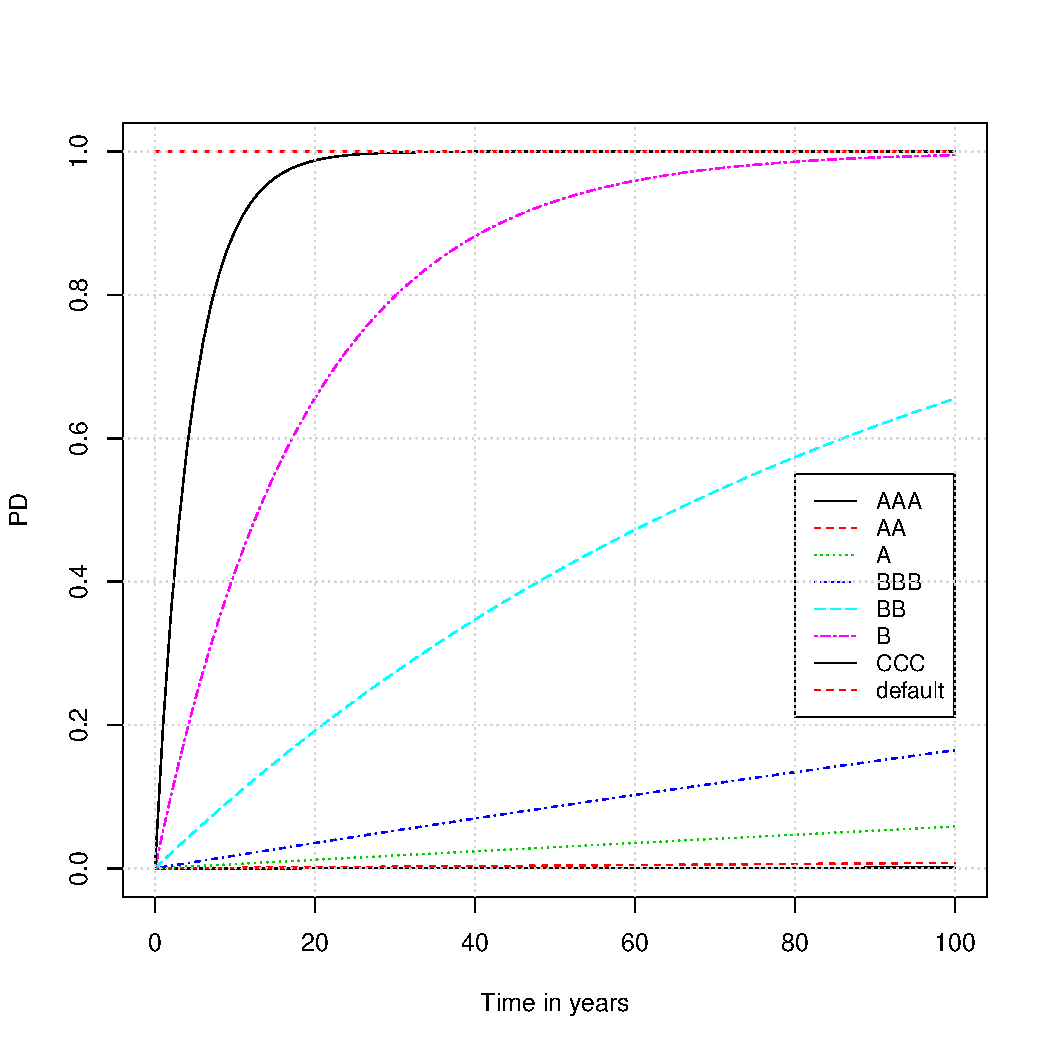
\includegraphics[width=7cm]{pdfsv1}
	}
	\subcaptionbox{Probability of Default (10-year zoom)}{
		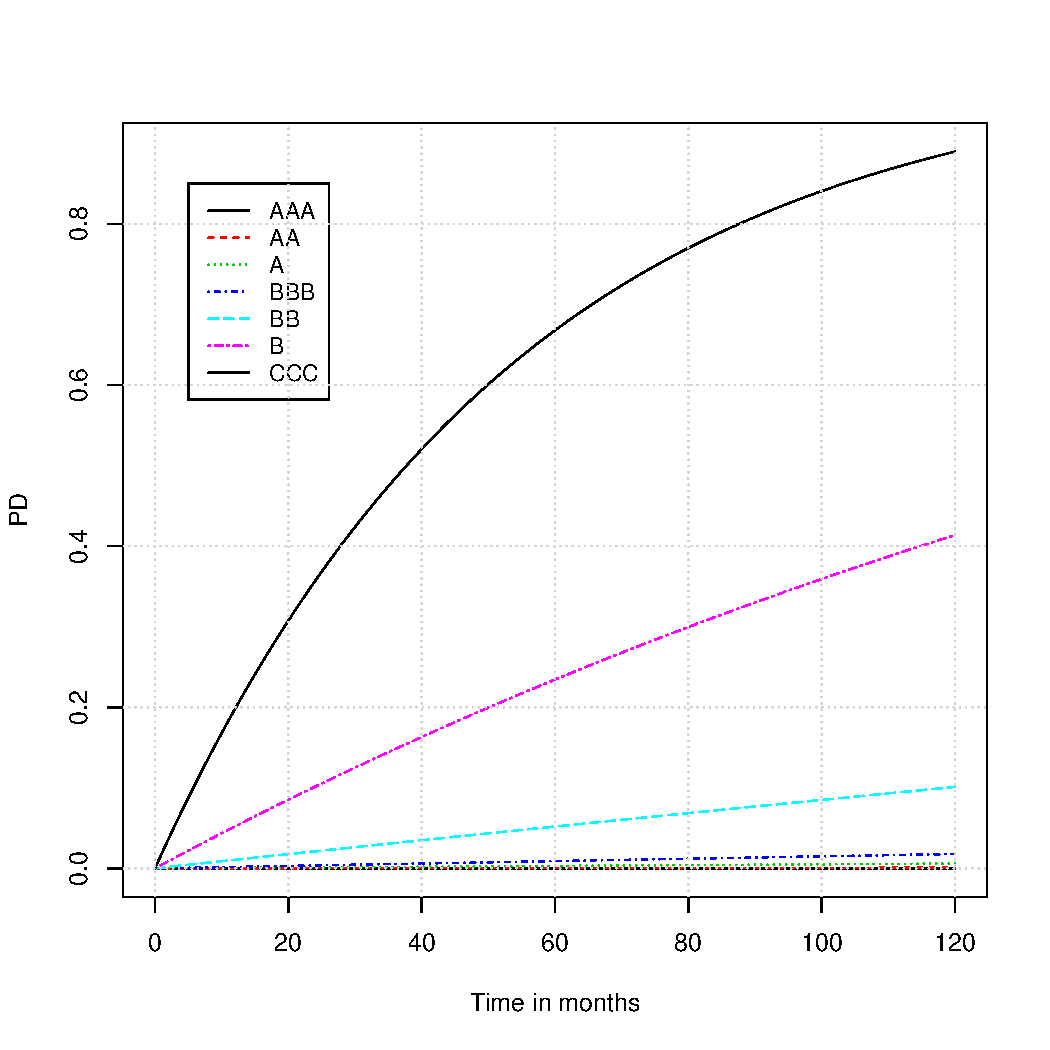
\includegraphics[width=7cm]{pdfsv2}
	}
	\caption{PDs derived from annual values}
	\label{fig:pdfsv}
\end{figure}

\subsection{Obtaining PDs from advanced models}

There are financial institutions that may have models to forecast the 
transition matrix using some economic indicators such as GDP or inflation. We 
note as $M_T(t)$ the T-period transition matrix at time $t$. In these cases, 
the time-until-default distributions can be obtained successively composing
the transition matrices for each T-period.
\begin{displaymath}
	F_i(t) = \Pr\{T_. \le t\} = \left(
		\left( \prod_{j=1}^{[t/T]} M_T(j) \right) \cdot 
		M_{t-T\cdot[t/T]}\left([t/T]+1\right) 
		\right)_{id}
\end{displaymath}
in which $[x]$ is the integer part of $x$, $T_.$ is the time-until-default
of an obligor with the i-th rating, $d$ is the index of the \emph{defaulted} 
rating, $M_t(j)$ is the T-period transition matrix evaluated at time $j$ 
and scaled to time $t$, and $(M)_{ij}$ is the matrix element located in the 
i-th row and the j-th column.

The time-until-default distributions derived from an advanced model may show 
various steps according to the different stages of the economic cycle. This 
approach is the most appropriate for risk estimates in the medium and long 
term.

CCruncher allows description of the PDs derived from advanced models specifying 
the PDs' values at given time points. These must fulfill the cdf conditions:
~\\
~\\
\storestyleof{itemize}
\begin{listliketab} 
	\begin{tabular}{Lll}
		\textbullet & $F_i(0) = 0$                 & $i=1,\dots,r \quad i \ne \text{default}$ \\
		\textbullet & $F_i(t)$ strictly increasing & $i=1,\dots,r \quad i \ne \text{default}$ \\
		\textbullet & $F_i(\infty) = 1$            & $i=1,\dots,r$ \\
		\textbullet & $F_{\text{default}}(t) = 1$  & $\forall\ t \ge 0$ \\
	\end{tabular} 
\end{listliketab}
~\\
~\\
The functions specified in this manner are interpolated using cubic splines
when the above conditions are preserved and are interpolated using linear 
splines when they are not.

%------------------------------------------------------------------------------
% COPULA BASICS
%------------------------------------------------------------------------------
\section{Copula Basics}
\label{ap:copula_basics}

\begin{wrapfigure}{r}{0.5\textwidth}
	\vspace{-25pt}
	\begin{center}
		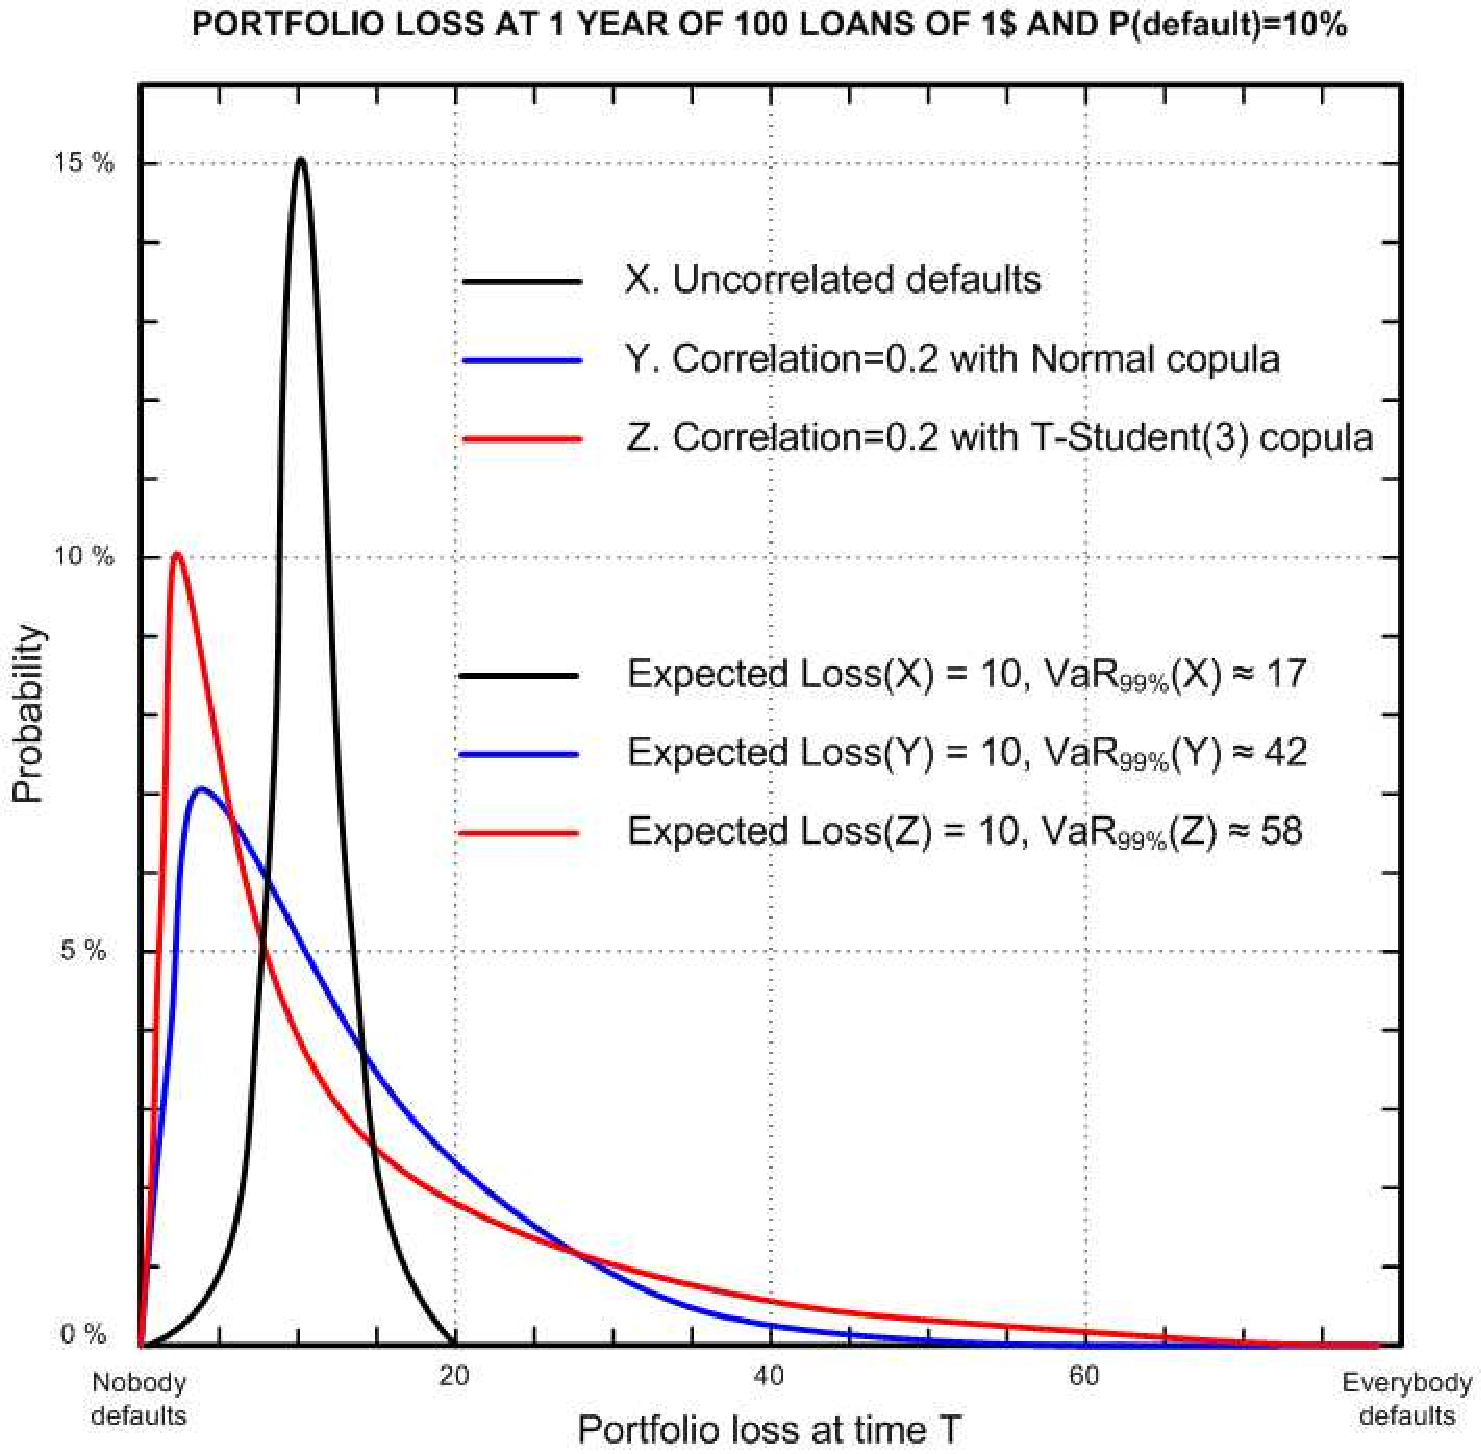
\includegraphics[width=0.48\textwidth]{ercim78}
	\end{center}
	\vspace{-10pt}
	\caption{Dependence structure effect}
	\vspace{-10pt}
	\label{fig:copula_effect}
\end{wrapfigure}
It is common to use correlation as a measure of dependency between random 
variables. In most cases, this measure does not fully reflect the structure 
of dependence between the variables. Figure~\ref{fig:copula_effect} displays 
two cases with the identical mean, marginals and correlations but a distinct 
risk profile because the two cases' underlying  dependence structure is 
distinct (Gaussian copula vs.\ t-Student(3) copula). The mathematical concept 
that does reflect the structure of dependence between random variables, 
however, is the copula, which we define below. The world of copulas is vast 
and quite interesting. See~\cite[chap. 5]{mcneil:2005} for a pleasant 
introduction to copulas.

\begin{definition}[Copula]
	A copula function $C$ is a multivariate distribution defined on the 
	unit hypercube $[0,1]^d$ with standard uniform marginals. 
	More precisely,
	\begin{displaymath}
		C(u_1, \dots, u_d) = \Pr\{U_1 \le u_1, \dots, U_d \le u_d\}
	\end{displaymath}
	in which $U_i \sim \text{Uniform}(0,1) \text{ for } i = 1,\dots, d$.
\end{definition}

Sklar's theorem~\cite{sklar:1959} states that any multivariate 
distribution with continuous marginals can be decomposed into the marginals and 
a copula that reflects the structure of dependence between them. Later, we will 
use this statement to define and simulate the t-Student copula.

\begin{theorem}[Sklar's theorem]
	\label{thm:sklar}
	Let $F$ be a $d$-dimensional distribution function with margins 
	$F_1,\dots,F_d$. Then there is a $d$-copula $C$ such that for all 
	$x \in \mathbb{R}^d$,
	\begin{displaymath}
		F(x_1,\dots,x_d) = C(F_1(x_1),\dots,F_d(x_d))
	\end{displaymath}
	If $F_1,\dots,F_d$ are all continuous, the $C$ is unique; otherwise, $C$ is 
	uniquely determined on $\text{Ran}F_1 \times \cdots \times \text{Ran}F_d$.
	Conversely, if $C$ is a $d$-copula and $F_1,\dots,F_d$ are distribution 
	functions, then the function $F$ defined above is a $d$-dimensional 
	distribution function with margins $F_1,\dots,F_d$.
\end{theorem}

\begin{corollary}[Copula of a multivariate distribution]
	\label{cor:cop1}
	Let $X=(X_1, \dots, X_d)$ be a random vector with a multivariate 
	distribution $F$ and continuous marginals $F_1, \dots, F_d$. 
	Then its copula is
	\begin{displaymath}
		C(u_1,\dots,u_d) = F(F_1^{-1}(u_1), \dots, F_d^{-1}(u_d))
	\end{displaymath}
\end{corollary}
%\begin{proof}
%This is a direct application of Sklar's theorem:
%\begin{displaymath}
%C(F_1(x_1), \dots, F_d(x_d)) = 
%F(F_1^{-1}(F_1(x_1)), \dots, F_d^{-1}(F_d(x_d))) = 
%F(x_1, \dots, x_d)
%\end{displaymath}
%\end{proof}

\begin{corollary}[Copula simulation]
	\label{cor:cop2}
	Let $X=(X_1, \dots, X_d)$ be a random vector with a multivariate 
	distribution $F$ and continuous marginals $F_1, \dots, F_d$.
	If we have a procedure to simulate $X$, then we can simulate 
	its copula $C$ using:
	\begin{displaymath}
		(U_1, \dots, U_d) = (F_1(X_1), \dots, F_d(X_d))
	\end{displaymath}
	in which $U_i$ are the copula components.
\end{corollary}

\begin{corollary}[Multivariate distribution simulation]
	\label{cor:cop3}
	Let $X=(X_1, \dots, X_d)$ be a random vector with a copula $C$
	and continuous marginals $F_1, \dots, F_d$. If we have a
	procedure to simulate $C$, then we can simulate $X$ using
	\begin{displaymath}
		(X_1, \dots, X_d) = (F_1^{-1}(U_1), \dots, F_d^{-1}(U_d))
	\end{displaymath}
	in which $U_i$ are the copula components.
\end{corollary}

\begin{definition}
	Spearman's rho is a measure of the linear relation between the two 
	variables $X$ and $Y$, and it is defined as the Pearson's correlation 
	coefficient between the ranked variables, $x$ and $y$:
	\begin{displaymath}
		\rho_s = \frac{\displaystyle \sum_i (x_i-\bar{x}) (y_i-\bar{y})}
		{\sqrt{\displaystyle \sum_i (x_i-\bar{x})^2 \sum_i (y_i-\bar{y})^2}}
	\end{displaymath}
	It has the important property that its value only relies on the underlying 
	copula $C$, not on marginals. It can be written as
	\begin{displaymath}
		\rho_s = 12 \displaystyle \int_0^1 \int_0^1 C(u,v) \ud u \ud v -3
	\end{displaymath}
\end{definition}

%------------------------------------------------------------------------------
% MULTIVARIATE t-STUDENT DISTRIBUTION
%------------------------------------------------------------------------------
\section{Multivariate t-Student Distribution}
\label{ap:mtsd}

The majority of the results presented below have been extracted 
from~\cite{kotz:2004,demarta:2005}.

\begin{definition}[Multivariate t-Student distribution]
	The $d$-dimensional random vector $X=(X_1,\dots,X_d)$ is said to have a 
	(non-singular) multivariate t-Student distribution with $\nu$ degrees of 
	freedom, mean vector $\vec{\mu}$ and positive-definite dispersion or 
	scatter matrix $\Sigma$, denoted $t_d(\nu,\vec{\mu},\Sigma)$, if its 
	density is given by
	\begin{displaymath}
		f(\vec{x})=\frac{\Gamma\left(\frac{\nu+d}{2}\right)}
		{\Gamma\left(\frac{\nu}{2}\right)\sqrt{(\pi \nu)^d |\Sigma|}}
		\left(
		1+ \frac{(\vec{x}-\vec{\mu})^\top\Sigma^{-1}(\vec{x}-\vec{\mu})}{\nu}
		\right)^{-\frac{\nu+d}{2}}
	\end{displaymath}
	in which $\Gamma$ is the gamma function and $|\Sigma|$ is the 
	determinant of the matrix.
\end{definition}

\begin{proposition}[t-Student covariance]
	The covariance matrix of the $X \sim t_d(\nu,\vec{\mu},\Sigma)$ is
	\begin{displaymath}
		\text{Cov}(X) = \frac{\nu}{\nu-2} \cdot \Sigma \quad \text{if} 
		\quad \nu > 2
	\end{displaymath}
\end{proposition}

\begin{proposition}[Gaussian as limit of the t-Student]
	The t-Student distribution converges to a Gaussian distribution 
	when $\nu$ tends to $\infty$.
	\begin{displaymath}
		\lim_{\nu \to \infty} t_d(\nu,\vec{\mu},\Sigma) = N(\vec{\mu},\Sigma)
	\end{displaymath}
\end{proposition}

\begin{proposition}[Multivariate t-Student characterization]
	\label{prop:mtschar}
	A random vector $T \sim t_d(\nu,\vec{\mu},\Sigma)$ can be expressed as:
	\begin{displaymath}
		T \stackrel{d}{=} \vec{\mu} + \sqrt{\frac{\nu}{V}}\cdot Z
		\quad \text{ where } Z \sim N(\vec{0},\Sigma) 
		\text{ and } V \sim \chi_{\nu}^2
	\end{displaymath}
\end{proposition}

\begin{proposition}[Multivariate t-Student marginals]
	Assume $X \sim t_d(\nu,\vec{0},\Sigma)$. Then its i-th marginal is 
	$X_i \sim t_1(\nu,0,\sigma_{ii})$.
\end{proposition}

\begin{definition}[t-Student copula]
	The t-Student copula, $C_{\nu,\Sigma}^{\text{t}}$, is the copula of the 
	multivariate t-Student distribution $t_d(\nu,\vec{\mu},\Sigma)$.
\end{definition}

\begin{proposition}[t-Student copula equivalence]
	The copula of $t_d(\nu,\vec{\mu},\Sigma)$ is identical to that of 
	$t_d(\nu,\vec{0},R)$ in which $R$ is the correlation matrix implied by 
	the dispersion matrix $\Sigma$.
\end{proposition}

\begin{proposition}[t-Student copula density]
	The t-Student copula, $C_{\nu,R}^{\text{t}}$, in which $R$ is a 
	correlation matrix, has the following distribution function:
	\begin{displaymath}
		C_{\nu,R}^{\text{t}}(u_1, \dots, u_d) = 
		\int_{-\infty}^{t_\nu^{-1}(u_1)} \dots \int_{-\infty}^{t_\nu^{-1}(u_d)} f(x) \ud x
	\end{displaymath}
	in which $f(x)$ is the density function of $t_d(\nu,\vec{0},R)$ and 
	$t_{\nu}^{-1}$ denotes the quantile function of the univariate distribution 
	$t_1(\nu,0,1)$. The copula density is
	\begin{displaymath}
		\label{eq:density}
		c_{\nu,R}^{\text{t}}(u_1,\dots,u_d) =
		|R|^{-\frac{1}{2}} 
		\displaystyle\frac{\Gamma{\left(\frac{\nu+d}{2}\right)}}{\Gamma{\left(\frac{\nu}{2}\right)}}
		\displaystyle\left[ \frac{\Gamma{\left(\frac{\nu}{2}\right)}}{\Gamma{\left(\frac{\nu+1}{2}\right)}} \right]^d
		\frac{\displaystyle\left( 1+\frac{\zeta' R^{-1} \zeta}{\nu}\right)^{-\frac{\nu+d}{2}}}{\displaystyle\prod_{i=1}^d \left( 1+\frac{\zeta_i^2}{\nu} \right)^{-\frac{\nu+1}{2}}}
	\end{displaymath}
	\noindent
	in which $\zeta=(t_\nu^{-1}(u_1), \dots, t_\nu^{-1}(u_d))$ is the vector 
	of the t-Student univariate inverse distribution functions.
\end{proposition}

%------------------------------------------------------------------------------
% COVARIANCE BLOCK MATRIX
%------------------------------------------------------------------------------
\section{Covariance Block Matrix}
\label{ap:cbm}

The content presented in this appendix is detailed and extended 
in~\cite{torrent:2011}.

\begin{definition}[Covariance block matrix]
	A matrix $A$ is a covariance block matrix $B_k(\vec{n},\vec{d},M)$
	in which:
	\begin{itemize}
		\item $\vec{n}=(n_1,\dots,n_k)$ with $n_i \in \mathbb{N}$ and $1 \le n_i$ (number of elements per block),
		\item $\vec{d}=(d_1,\dots,d_k)$ with $d_i \in \mathbb{R}$ (diagonal block values), and
		\item $M$ is a $k {\times} k$ symmetric matrix with values $m_{ij} \in \mathbb{R}$ (block values)
	\end{itemize}
	when
	\begin{itemize}
		\item each block $B_{ij}$ is an $n_i {\times} n_j$ constant matrix with value $m_{ij}$
		\item diagonal blocks $B_{ii}$ have diagonal values $d_i$
		\item A is definite-positive.
	\end{itemize}
\end{definition}

\begin{example}[Correlation block matrix]
	\label{example1}
	We have $6$ obligors sorted by sector. The first three belong to the 
	banking sector, the next two belong to the energy sector 
	and the last one belongs to the services sector. Obligors default time
	dependence is determined only by sectors. Thus, the correlation matrix 
	of the underlying elliptical copula is a correlation block matrix.
	\small
	\begin{displaymath}
		\left.
		\begin{array}{l}
			\vec{n} = \left(3,2,1\right) \\
			\vec{d} = \left(1,1,1\right) \\
			M = \left(
			\begin{array}{ccc}
				0.5 & 0.2  & 0.1  \\
				0.2 & 0.4  & 0.15 \\
				0.1 & 0.15 & 0.5  \\
			\end{array}
			\right)
		\end{array}
		\right\}
		\rightarrow
		B_3(\vec{n},\vec{d},M)=
		\left(
		\begin{array}{ccc|cc|c} 
			1   & 0.5 & 0.5 & 0.2  & 0.2  & 0.1  \\ 
			0.5 & 1   & 0.5 & 0.2  & 0.2  & 0.1  \\ 
			0.5 & 0.5 & 1   & 0.2  & 0.2  & 0.1  \\ 
			\hline
			0.2 & 0.2 & 0.2 & 1    & 0.4  & 0.15 \\ 
			0.2 & 0.2 & 0.2 & 0.4  & 1    & 0.15 \\ 
			\hline
			0.1 & 0.1 & 0.1 & 0.15 & 0.15 & 1    
		\end{array} 
		\right)
	\end{displaymath}
\end{example}

\begin{proposition}[Covariance block matrix eigenvalues]
	\label{prop1}
	Let $A = B_k(\vec{n}, \vec{d}, M)$ a non-singular matrix, and let $G$ be 
	the $k {\times} k$ deflated matrix
	\begin{displaymath}
		G =
		\left( \begin{array}{cccc}
		d_1+(n_1-1)\cdot m_{11} & n_2 \cdot m_{12}        & \cdots & n_k \cdot m_{1k} \\
		n_1\cdot m_{21}         & d_2+(n_2-1)\cdot m_{22} & \cdots & n_k \cdot m_{2k} \\
		\vdots                  & \vdots                  & \ddots & \vdots \\
		n_1\cdot m_{k1}         & n_2 \cdot m_{k2}        & \cdots & d_k+(n_k-1)\cdot m_{kk} \\
		\end{array} \right)
	\end{displaymath}
	Then, the eigenvalues of $A$ are as follows:
	\begin{itemize}
		\item $d_{i}-m_{ii}$ with multiplicity $n_i-1$ for $i=1,\dots,k$.
		\item $\lambda_i$, the eigenvalues of $G$ with multiplicity $1$.
	\end{itemize}
\end{proposition}

\begin{corollary}
	A covariance block matrix $B_k(\vec{n},\vec{d},M)$ is definite-positive if
	\begin{itemize}
		\item $d_i > m_{ii}$ for all $i=1,\dots,k$, and
		\item the deflated matrix $G$ is definite-positive.
	\end{itemize}
\end{corollary}

%------------------------------------------------------------------------------
% MULTI-FACTOR GAUSSIAN MODEL
%------------------------------------------------------------------------------
\section{Multi-Factor Gaussian Model}
\label{ap:mfgm}
~\\
\begin{definition}[Gaussian multi-factor model]
	\label{def:gmfm}
	We say that a multivariate distribution $X$ follows a Gaussian multi-factor
	model if it can be expressed in this form:
	\begin{displaymath}
		X_i^j = w_i \cdot Z_i + \sqrt{1-w_i^2} \cdot \epsilon_i^j
		\quad \text{ where } \left\{
		\begin{array}{ll}
			i = 1, \dots, k & \text{$k$ is the number of factors} \\
			j = 1, \dots, n_i & \text{$n_i$ is i-th factor size} \\
			Z \sim N(\vec{0},R) & \text{$R$ is a $k {\times} k$ correlation matrix} \\
			w_i \in (0,1) & \text{the factor loadings } \\
			\epsilon_i^j \sim N(0,1) \text { iid } & \forall\ i,j \\
			Z, \epsilon_i^j \text{ independents } & \forall\ i,j \\
		\end{array}
		\right.
	\end{displaymath}
	An alternative definition based on the covariance matrix is
	\begin{displaymath}
		X_i^j = Z_i + \sqrt{1-\Sigma_{ii}} \cdot \epsilon_i^j
		\quad \text{ where } \left\{
		\begin{array}{ll}
			i = 1, \dots, k & \text{$k$ is the number of factors} \\
			j = 1, \dots, n_i & \text{$n_i$ is i-th factor size} \\
			Z \sim N(\vec{0},\Sigma) & \text{$\Sigma$ is a $k {\times} k$ covariance matrix} \\
			\Sigma_{ii} \in (0,1) & \text{diagonal values of $\Sigma$} \\
			\epsilon_i^j \sim N(0,1) \text { iid } & \forall\ i,j \\
			Z, \epsilon_i^j \text{ independents } & \forall\ i,j \\
		\end{array}
		\right.
	\end{displaymath}
\end{definition}

\begin{proposition}[The Gaussian multi-factor model is a Gaussian distribution]
	\label{prop:gmfigs}
	The Gaussian multi-factor model defined by factor loadings $\vec{w}$,
	the factor correlation matrix $R$, and $n = \sum_{i=1}^k n_i$ is a 
	multivariate Gaussian distribution with an $n {\times} n$ block 
	correlation matrix $\widehat{R}=B_k(\vec{n},\vec{1},\Sigma)$ 
	with values $\Sigma_{ij} = w_i \cdot w_j \cdot R_{ij}$.
\end{proposition}
\begin{proof}
	We check that the correlation between components of the Gaussian multi-factor 
	model fulfill the equivalence.
	
	Version with the correlation matrix $R$:
	\begin{displaymath}
		\begin{array}{rl}
			\text{Var}(X_i^j) =                       &
			w_i^2 \cdot \text{Var}(Z_i) + (1-w_i^2) \cdot \text{Var}(\epsilon_i^j) +
			2 \cdot w_i \cdot \sqrt{1-w_i^2} \cdot \text{Cov}(Z_i, \epsilon_i^j)    \\
			=                                         & w_i^2 + (1-w_i^2) = 1       \\
		\end{array}
	\end{displaymath}
	\begin{displaymath}
		\begin{array}{rl}
			\text{Cor}(X_{i_1}^{j_1},X_{i_2}^{j_2}) = & \text{Cov}(X_{i_1}^{j_1},X_{i_2}^{j_2})                                               \\
			=                                         & w_{i_1} \cdot w_{i_2} \cdot \text{Cov}(Z_{i_1},Z_{i_2}) +
			                                            w_{i_1} \cdot \sqrt{1-w_{i_2}^2} \cdot \text{Cov}(Z_{i_1}, \epsilon_{i_2}^{j_2}) +    \\
			                                          & + \sqrt{1-w_{i_1}^2} \cdot w_{i_2} \cdot \text{Cov}(\epsilon_{i_1}^{j_1}, Z_{i_2}) +
			                                            \sqrt{1-w_{i_1}^2} \cdot \sqrt{1-w_{i_2}^2} \cdot 
			                                            \text{Cov}(\epsilon_{i_1}^{j_1}, \epsilon_{i_2}^{j_2})                                \\
			=                                         & w_{i_1} \cdot w_{i_2} \cdot \text{Cov}(Z_{i_1}, Z_{i_2})                              \\
			=                                         & w_{i_1} \cdot w_{i_2} \cdot R_{i_1i_2}                                                \\
		\end{array}
	\end{displaymath}
	Version with the covariance matrix $\Sigma$:
	\begin{displaymath}
		\begin{array}{rl}
			\text{Var}(X_i^j) =                       &
			\text{Var}(Z_i) + (1-\Sigma_{ii}) \cdot \text{Var}(\epsilon_i^j) +
			2 \cdot \sqrt{1-\Sigma_{ii}} \cdot \text{Cov}(Z_i, \epsilon_i^j)               \\
			=                                         & \Sigma_{ii} + (1-\Sigma_{ii}) = 1  \\
		\end{array}
	\end{displaymath}
	\begin{displaymath}
		\begin{array}{rl}
			\text{Cor}(X_{i_1}^{j_1},X_{i_2}^{j_2}) = & \text{Cov}(X_{i_1}^{j_1},X_{i_2}^{j_2})                                        \\
			=                                         & \text{Cov}(Z_{i_1},Z_{i_2}) +
			                                            \sqrt{1-\Sigma_{i_2i_2}} \cdot \text{Cov}(Z_{i_1}, \epsilon_{i_2}^{j_2}) +     \\
			                                          & + \sqrt{1-\Sigma_{i_1i_1}} \cdot \text{Cov}(\epsilon_{i_1}^{j_1}, Z_{i_2}) +
			                                            \sqrt{1-\Sigma_{i_1i_1}} \cdot \sqrt{1-\Sigma_{i_2i_2}} \cdot 
			                                            \text{Cov}(\epsilon_{i_1}^{j_1}, \epsilon_{i_2}^{j_2})                         \\
			=                                         & \Sigma_{i_1i_2}                                                                \\
		\end{array}
	\end{displaymath}
	The characterization of the multivariate Gaussian~\cite[thm. 2.6.2]{anderson:1984}
	posits that if every linear combination of the components of a 
	vector $X$ is normally distributed, then $X$ is normally distributed.
	It is straightforward to check that the multi-factor Gaussian model 
	fulfills this property and consequently is a multivariate Normal.
	\\
\end{proof}

\begin{proposition}[Gaussian multi-factor model $\subsetneq$ multivariate Gaussian block]
	\label{prop:ibne}
	Any multi-factor model can be expressed as a multivariate Gaussian 
	block; however, there are multivariate Gaussian blocks that cannot be 
	expressed as a Gaussian multi-factor model.
\end{proposition}
\begin{proof}
	Proposition~\ref{prop:gmfigs} states that any multi-factor model 
	is a multivariate Gaussian composed of blocks.
	Next we see that the reciprocal is false. Let 
	$\widehat{R} = B_k(\vec{n},\vec{1},\Sigma)$, the Gaussian distribution 
	correlation matrix. We use the equivalence 
	$\Sigma_{ij} = w_i \cdot w_j \cdot R_{ij}$ stated in 
	proposition~\ref{prop:gmfigs} to determine the cases that cannot be 
	expressed as a multi-factor model.

	\textbf{Case 1}. Factor loadings with imaginary values.
	\begin{displaymath}
		\Sigma_{ii} = w_i \cdot w_i \cdot R_{ii} = w_i^2
	\end{displaymath}
	\begin{adjustwidth}{1cm}{0pt}
		If $\Sigma_{ii}$ is negative, then $w_i$ has an imaginary value.
		For example,
	\end{adjustwidth}
	\begin{displaymath}
		\widehat{R} = \left(
		\begin{array}{cc|c}
			1    & -0.5 & 0 \\
			-0.5 & 1    & 0 \\
			\hline
			0    & 0    & 1 \\
		\end{array}
		\right) 
		\longrightarrow
		R = \left(
		\begin{array}{cc}
			1 & 0 \\
			0 & 1 \\
		\end{array}
		\right)
		\text{ , }
		w = (\sqrt{-0.5}, 1)
		\text{ !!}
	\end{displaymath}
	
	\textbf{Case 2}. Factors correlation with absolute value > 1.
	\begin{displaymath}
		\Sigma_{ij} = w_i \cdot w_j \cdot R_{ij} \longrightarrow 
		R_{ij} = \frac{\Sigma_{ij}}{w_i \cdot w_j} = 
		\frac{\Sigma_{ij}}{\sqrt{\Sigma_{ii} \cdot \Sigma_{jj}}}
	\end{displaymath}
	\begin{adjustwidth}{1cm}{0pt}
		If $\Sigma_{ij}^2 > \Sigma_{ii} \cdot \Sigma_{jj}$, then $R_{ij}$ has an 
		absolute value larger than 1, which is not possible because $R_{ij}$ 
		is a correlation value. For example,
	\end{adjustwidth}
	\begin{displaymath}
		\widehat{R} = \left(
		\begin{array}{cc|cc}
			1   & 0.5 & 0.6 & 0.6 \\
			0.5 & 1   & 0.6 & 0.6 \\
			\hline
			0.6 & 0.6 & 1   & 0.5 \\
			0.6 & 0.6 & 0.5 & 1   \\
		\end{array}
		\right) 
		\longrightarrow
		R = \left(
		\begin{array}{cc}
			1               & \frac{0.6}{0.5} \\
			\frac{0.6}{0.5} & 1               \\
		\end{array}
		\right)
		\text{ !!}
		\text{ , }
		w = (\sqrt{0.5}, \sqrt{0.5})
	\end{displaymath}
\end{proof}

It is disturbing that multivariate block Gaussian distributions exist
that cannot be expressed as a multi-factor model. Fortunately, the 
cases in which this occurs have no practical application to credit risk
modeling in which the number of obligors in each block is higher. 
The following proposition clarifies this theme.

\begin{proposition}[Gaussian multi-factor model $\approx$ multivariate Gaussian block]
	\label{prop:gmfamgb}
	Assume $X \sim N(\vec{0},\widehat{R})$ in which 
	$\widehat{R}=B_k(\vec{n},\vec{1},\Sigma)$ is a correlation block matrix. 
	Then $X$ can be expressed as a multi-factor Gaussian model if $n_i$ 
	values are large enough.
\end{proposition}
\begin{proof}
	We revise the cases in which the multivariate Gaussian distribution cannot
	be expressed as a multi-factor model, and we use proposition~\ref{prop1}
	to ascertain that if $n_i$ values are large enough, then 
	that is indeed a valid multi-factor model.
	
	\textbf{Case 1}. Factor loadings with imaginary values.
	\begin{adjustwidth}{1cm}{0pt}
		Factor loading $w_i$ with imaginary value is caused by $\Sigma_{ii} < 0$. 
		We use proposition~\ref{prop1} to determine the restrictions regarding 
		$\Sigma_{ii}$. We assume a unique factor.
		Because $\widehat{R}$ is a covariance block matrix definite-positive, 
		the deflated matrix has a positive determinant. Then,
	\end{adjustwidth}
	\begin{displaymath}
		\begin{array}{l}
			1 + (n_1-1) \cdot \Sigma_{11} > 0
			\\
			\Sigma_{11} > \frac{-1}{n_1-1} 
			\\
			\text{tending } n_1 \to \infty
			\\
			\Sigma_{11} \ge 0
		\end{array}
	\end{displaymath}
	
	\textbf{Case 2}. Factors correlation with absolute value > 1.
	\begin{adjustwidth}{1cm}{0pt}
		A factor correlation larger than $1$ is caused by 
		$R_{12} = \frac{\Sigma_{12}}{\sqrt{\Sigma_{11} \cdot \Sigma_{22}}}$
		in which $\Sigma_{12}^2 > \Sigma_{11} \cdot \Sigma_{22}$.
		We use proposition~\ref{prop1} to determine the restrictions regarding 
		$\Sigma_{12}$. Because $\widehat{R}$ is covariance block matrix 
		definite-positive, the deflated matrix has a positive determinant. 
		Then,
	\end{adjustwidth}
	\begin{displaymath}
		\begin{array}{l}
			1 + (n_1-1) \cdot \Sigma_{11} + (n_2-1) \cdot \Sigma_{22} +
			(n_1-1) \cdot (n_2-1) \cdot \Sigma_{11} \cdot \Sigma_{22} -
			n_1 \cdot n_2 \cdot \Sigma_{12}^2 > 0
			\\
			\Sigma_{12}^2 <
			\frac{1}{n_1 \cdot n_2} +
			\frac{(n_1-1)}{n_1 \cdot n_2} \cdot \Sigma_{11} +
			\frac{(n_2-1)}{n_1 \cdot n_2} \cdot \Sigma_{22} +
			\frac{(n_1-1) \cdot (n_2-1)}{n_1 \cdot n_2} \cdot \Sigma_{11} \cdot \Sigma_{22}
			\\
			\text{tending } n_1 \to \infty \text{ and } n_2 \to \infty
			\\
			\Sigma_{12}^2 \le \Sigma_{11} \cdot \Sigma_{22}
		\end{array}
	\end{displaymath}
\end{proof}

%------------------------------------------------------------------------------
% METROPOLIS-HASTINGS ALGORITHM
%------------------------------------------------------------------------------
\section{Metropolis-Hastings Algorithm}
\label{ap:mha}

This section contains a brief introduction to Bayesian inference using 
the Metropolis-Hastings algorithm and is heavily influenced by the book 
\emph{Bayesian Modeling Using WinBUGS}~\cite{ntzoufras:2009}.

Bayesian statistics differ from classical statistical theory because all 
unknown parameters are considered as random variables. We want to calculate 
the distribution $f(\theta \mid y)$ of the parameters $\theta$ given the 
observed data $y$. According to the Bayes theorem, this can be written as
\begin{displaymath}
	f(\theta \mid y) = \frac{f(y \mid \theta) \cdot f(\theta)}{f(y)} \propto f(y \mid \theta) \cdot f(\theta)
\end{displaymath}

We call \emph{posterior distribution} to $f(\theta \mid y)$ and 
\emph{prior distribution} to $f(\theta)$. This prior distribution 
expresses the information available to the researcher before 
any data are involved in the statistical analysis. $f(y \mid \theta)$ 
is the probability of observing $y$ given $\theta$ and is also 
known as the likelihood.
\begin{displaymath}
	f(y \mid \theta) = \prod_{i=1}^n f(y_i \mid \theta)
\end{displaymath}

When utilizing Bayesian inference, we can identify a closed form of the 
posterior distribution in only a few cases. Generally this must be determined 
by numerical methods. One of the most used is the Metropolis-Hastings (M-H)
algorithm, which belongs to the family of Markov Chain Monte Carlo (MCMC) 
methods. These methods are based on the construction of a Markov chain that 
converges on the target distribution, which, in our case, is the posterior 
distribution.

\begin{definition}[Markov chain]
	A Markov chain is a stochastic process 
	$\left\{\theta^{(1)},\dots,\theta^{(T)}\right\}$ such that
	\begin{displaymath}
		f\left(\theta^{(t+1)} \mid \theta^{(t)},\dots,\theta^{(1)}\right) = 
		f\left(\theta^{(t+1)} \mid \theta^{(t)}\right)
		\text{,}
	\end{displaymath}
	that is, the distribution of $\theta$ at sequence $t+1$, given all the 
	preceding $\theta$ values, depends only on the previous value. 
	When the Markov chain is irreducible, aperiodic, and positive-recurrent, 
	the distribution of $\theta^{(t)}$ converges on its equilibrium 
	distribution, which is independent of the initial values of the chain 
	$\theta^{(0)}$.
\end{definition}

The Markov chain is not an unfamiliar concept to us because the transition 
matrix (see definition~\ref{def:tm}) is a Markov chain in which its 
equilibrium state is the \emph{defaulted} rating (i.e., just any 
obligor ends up defaulting), allowing us to consider the PDs as cdfs.
The Metropolis-Hastings algorithm generates a sample from $f(\theta)$ 
by constructing a Markov chain that has $f(\theta)$ as the equilibrium 
distribution.

\begin{algorithm}[Metropolis-Hastings]
	Let us assume a target distribution $f(x)$ from which we wish to 
	generate a sample $\left\{x^{(0)},\dots,x^{(T)}\right\}$. The 
	Metropolis-Hastings algorithm can be described by the following 
	iterative procedure:
	\begin{enumerate}
		\item Set initial values $x^{(0)}$
		\item For $t=1,\dots,T$ repeat the following steps:
		\begin{itemize}
			\item Set $x=x^{(t-1)}$
			\item Let $x'$ be a random value from the proposal distribution 
			$q(x \to x')=q(x' \mid x)$
			\item Calculate the acceptance rate 
			$\alpha = \min\left(1,\frac{f(x') \cdot q(x \mid x')}{f(x) \cdot q(x' \mid x)}\right)$
			\item Update $x^{(t)}=\left\{
			\begin{array}{ll}
				x'        & \text{ with probability } \alpha   \\
				x^{(t-1)} & \text{ with probability } 1-\alpha 
			\end{array}\right.$ 
		\end{itemize}
	\end{enumerate}
\end{algorithm}

Because this is a Markov chain, the chosen starting point $x^{(0)}$ is 
irrelevant because the algorithm converges on the target distribution
no matter the starting point. If the starting point has low probability 
in respect to the target distribution, then the initial samples do not 
come from the equilibrium distribution and must be discarded until there 
is not equilibrium. We call the first $B$ iterations eliminated from the 
sample the \emph{burn-in period} for this reason.

\textbf{Bayesian inference}.
The Metropolis-Hastings algorithm outlined above can be directly implemented 
to conduct Bayesian inference by substituting $x$ with the unknown parameters 
$\theta$ and the target distribution $f(x)$ with the posterior distribution 
$f(\theta \mid y)$. Then, using the Bayes theorem, the acceptance rate 
becomes
\begin{displaymath}
	\alpha = \min\left(1,\frac{f(\theta' \mid y) \cdot q(\theta \mid \theta')}{f(\theta \mid y) \cdot q(\theta' \mid \theta)}\right) = \min\left(1,\frac{f(y \mid \theta') \cdot f(\theta') \cdot q(\theta \mid \theta')}{f(y \mid \theta)  \cdot f(\theta) \cdot q(\theta' \mid \theta)}\right)
\end{displaymath}

\textbf{Random-walk Metropolis-Hastings} is a special case with symmetrical 
proposals $q(\theta' \mid \theta) = q(\theta \mid \theta')$ in which 
$q(\theta' \mid \theta) \equiv N(\theta,\sigma)$. 
In this case, the acceptance rate depends only on the posterior distribution
and in the Bayesian inference case becomes
\begin{displaymath}
	\alpha = 
	\min\left(1,\frac{f(y \mid \theta') \cdot f(\theta') \cdot q(\theta \mid \theta')}{f(y \mid \theta)  \cdot f(\theta) \cdot q(\theta' \mid \theta)}\right) = 
	\min\left(1,\frac{f(y \mid \theta') \cdot f(\theta')}{f(y \mid \theta) \cdot f(\theta)}\right)
\end{displaymath}

The random walk fixes the shape of the proposal distribution and requires 
specifying the value $\sigma$. This value has a direct non-linear effect 
on the acceptance ratio (\#accepted/\#iterations). There is an optimal 
acceptance ratio that minimizes the auto-correlation and in most cases 
relies on the interval $[0.234,0.44]$. To avoid the  manual tuning of the 
scale parameter $\sigma$, we use the Robbins-Monro algorithm~\cite{garthwaite:2010}, 
which performs an adaptive scaling to achieve the desired acceptance ratio.

\begin{proposition}[The Robbins-Monro process]
	To achieve an acceptance ratio $p$ in the random-walk 
	Metropolis-Hastings algorithm, consider the following adaptive
	procedure:
	\begin{displaymath}
		\sigma^{(t+1)} = \left\{
		\begin{array}{ll}
			\sigma^{(t)} \cdot \left( 1 + \frac{1}{p \cdot t} \right) & \text{if $\theta'$ is accepted} \\
			\sigma^{(t)} \cdot \left( 1 - \frac{1}{(1-p) \cdot t} \right) & \text{if $\theta'$ is rejected} \\
		\end{array}
		\right.
	\end{displaymath}
	in which the starting value $\sigma^{(1)} > 0$ has an arbitrary value.
\end{proposition}

\textbf{Metropolis-Hastings using logarithms}.
The product of functions involves complicated expressions and accuracy 
problems. Therefore, it is usual to operate with logarithms. The 
logarithmic version of the acceptance rate in the Bayesian inference 
case becomes
\begin{displaymath}
	\begin{array}{rl}
		\ln(\alpha) = & \min \left( \ln(1),  
		\ln \left(\frac{f(y \mid \theta') \cdot f(\theta')}{f(y \mid \theta) \cdot f(\theta)}\right)
		\right) = \\
		= & \min \left( 0,
		\ln f(y \mid \theta') + \ln f(\theta') - \ln f(y \mid \theta) - \ln f(\theta)
		\right)
	\end{array}
\end{displaymath}

\textbf{The single-component Metropolis-Hastings} algorithm consists of updates 
of sequentially univariate components using Metropolis-Hastings steps. 
One generated observation $\theta^{(t)}$ is obtained after updating all 
components of the parameter vector. Generally, the sequence of updating the 
elements of $\theta$ does not influence the convergence of the algorithm.
Nevertheless, to ensure randomness, a random selection of the updating 
sequence is recommended. We use the notation $\theta_{\backslash j}$ to 
indicate the vector $\theta$, excluding its j-th component [ $\theta_{\backslash j}
= (\theta_1,\dots,\theta_{j-1},\theta_{j+1},\dots,\theta_{d})$ ].

\begin{algorithm}[Bayesian inference using Metropolis-Hastings] 
	\label{alg:bimh}
	Let $f(y \mid \theta)$ be the likelihood function, with priors 
	$f_j(\theta_j)$ and desired acceptance ratios $p_j$. Then the 
	parameters distribution can be sampled using the following 
	Metropolis-Hastings algorithm:
	\begin{enumerate}
		\item Set initial values $\theta^{(0)}$
		\item Set initial values $\sigma^{(0)}$
		\item For $t=1,\dots,T$ repeat the following steps:
		\begin{itemize}
			\item Set $\theta=\theta^{(t-1)}$
			\item Shuffle the update sequence
			\item For $j=1,\dots,d$ repeat the following steps:
			\begin{enumerate}[label=\alph*.]
				\item $\theta_j' = N(\theta_j,\sigma_j)$
				\item Calculate the logarithm of the acceptance rate \\
				$\ln(\alpha) = 
					\ln f(y \mid \theta_j',\theta_{\backslash j}) + 
					\ln f_j(\theta_j'\ ;\ \theta_{\backslash j}) - 
					\ln f(y \mid \theta_j,\theta_{\backslash j}) - 
					\ln f_j(\theta_j\ ; \ \theta_{\backslash j})
				$
				\item Simulate $u \sim U(0,1)$
				\item Update $\theta_j=\left\{
				\begin{array}{ll}
					\theta_j' & \text{ if } \ln(u) < \ln(\alpha) \\
					\theta_j  & \text{ otherwise }               
				\end{array}\right.$ 
				\item Update $\sigma_j^{(t)} = \left\{
					\begin{array}{ll}
						\sigma_j^{(t-1)} \cdot \left( 1 + \frac{1}{p_j \cdot t} \right) & \text{ if } \ln(u) < \ln(\alpha) \\
						\sigma_j^{(t-1)} \cdot \left( 1 - \frac{1}{(1-p_j) \cdot t} \right) & \text{ otherwise } \\
					\end{array}
				\right.$
			\end{enumerate}
			\item Set $\theta^{(t)}=\theta$
		\end{itemize}
	\end{enumerate}
\end{algorithm}

The simulated values from the posterior distribution have ergodic properties;
however, they are not independents. Independent values can be obtained by 
plotting the autocorrelation function (ACF) and estimating the length, $B$, 
for which the autocorrelation is canceled. Then only the values whose index 
is a multiple of $B$ are considered. Notably, the estimated parameters are 
not independent of one another; in fact, they form a multivariate distribution.

\begin{example}[Beta distribution calibration]
	We have a sample $\{y_1,\dots,y_{100}\}$ coming from a $\text{Beta}(2,5)$ 
	distribution. We want to perform Bayesian inference to determine the value 
	of the parameters $\alpha$ and $\beta$ using the Metropolis-Hastings 
	algorithm presented above. The density of the Beta distribution is
	\begin{displaymath}
		f(x\ ;\ \alpha, \beta) = 
		\frac{\Gamma(\alpha+\beta)}{\Gamma(\alpha) \cdot \Gamma(\beta)} 
		\cdot x^{(\alpha-1)} \cdot (1-x)^{(\beta-1)}
	\end{displaymath}
	The log-likelihood function, then, is
	\begin{displaymath}
		\ln f(y \mid \alpha, \beta) = 
		\displaystyle \sum_{i=1}^{100} 
		\ln \Gamma(\alpha+\beta) - \ln \Gamma(\alpha) - \ln \Gamma(\beta) +
		(\alpha-1) \cdot \ln(y_i) + (\beta-1) \cdot \ln(1-y_i)
	\end{displaymath}
	We know that $\alpha \in (0,10)$ and $\beta \in (0,30)$. Therefore, we 
	consider that prior distributions $f_{\alpha}()$ and $f_{\beta}()$ are 
	uniform distributions. Then,
	\begin{displaymath}
		\begin{array}{l}
			\ln f_{\alpha}(\alpha \ ;\ \beta) = \ln(\frac{1}{10})
			\\
			\ln f_{\beta}(\beta \ ;\ \alpha) = \ln(\frac{1}{30})
		\end{array}
	\end{displaymath}
	We apply the algorithm~\ref{alg:bimh} with starting point 
	$\left(\alpha^{(0)},\beta^{(0)}\right)=(1,1)$ and 
	desired acceptance ratios $(p_{\alpha},p_{\beta})=(0.3,0.3)$.
	Figure~\ref{fig:mhbd} displays the results after \num{25000} iterations.
	Notably, the first 500 iterations are not valid because the Markov 
	chain has not achieved the equilibrium distribution. These must be 
	considered in the burn-in period. The histograms of the sampled values
	approximate the parameters distribution that we are inferring.
\end{example}

\begin{figure}[!ht]
	\centering
	\subcaptionbox{Iterations 1--1000 of parameters $\alpha$ and $\beta$}{
		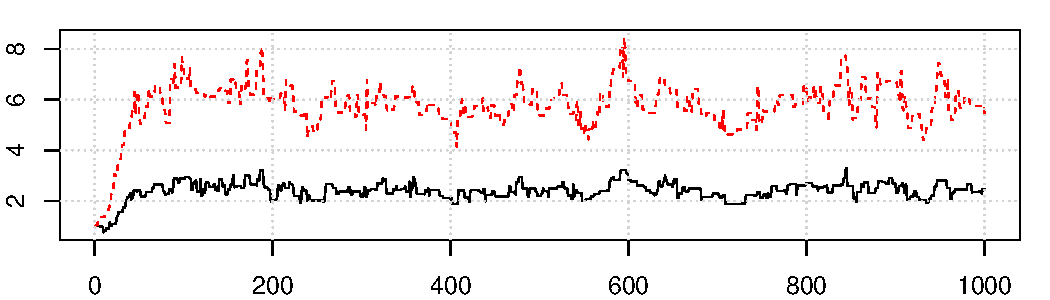
\includegraphics[width=0.98\textwidth]{mhbd1}
	}
	\\
	\subcaptionbox{Parameter $\alpha$ histogram}{
		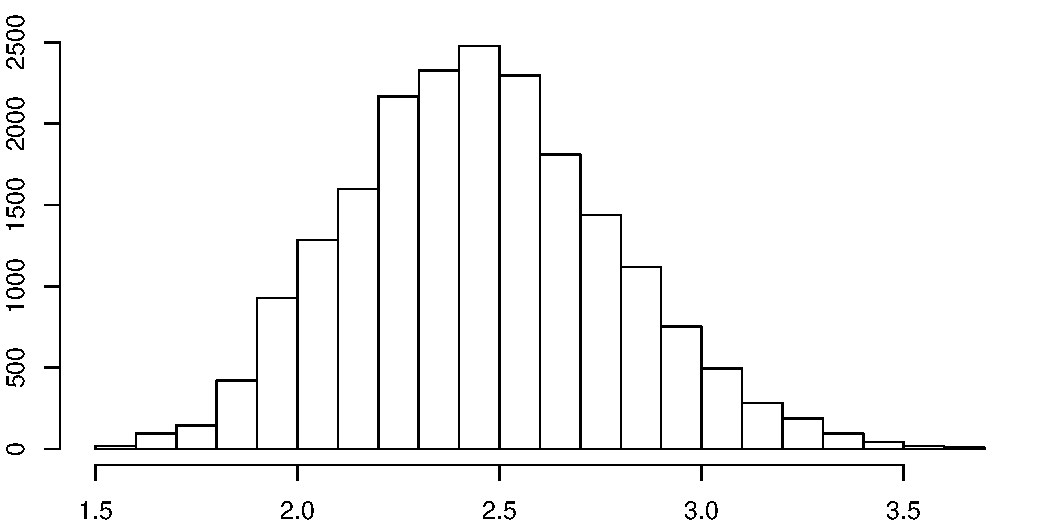
\includegraphics[width=7cm]{mhbd3}
	}
	\subcaptionbox{Parameter $\beta$ histogram}{
		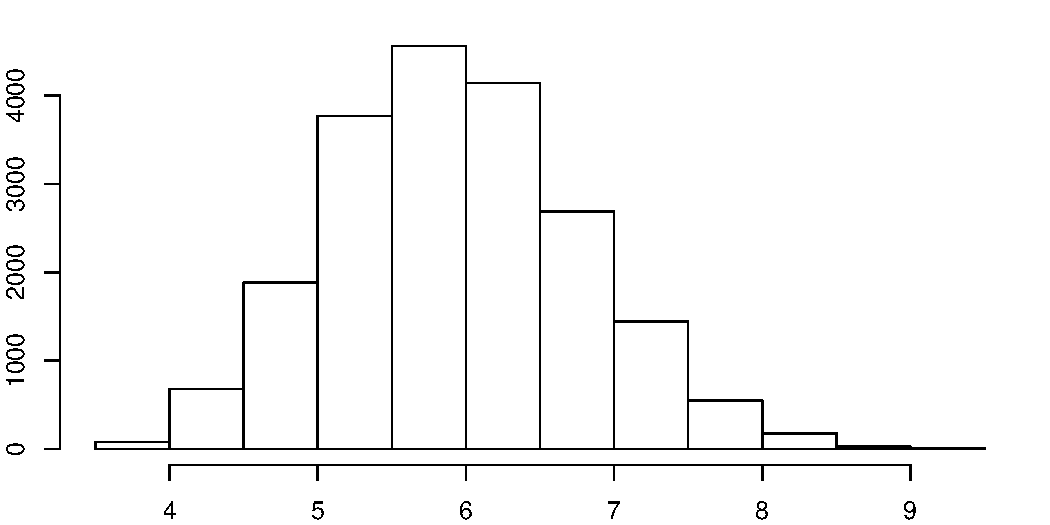
\includegraphics[width=7cm]{mhbd4}
	}
	\\
	\subcaptionbox{Iterations 1--1000 of scales $\sigma_{\alpha}$ and $\sigma_{\beta}$}{
		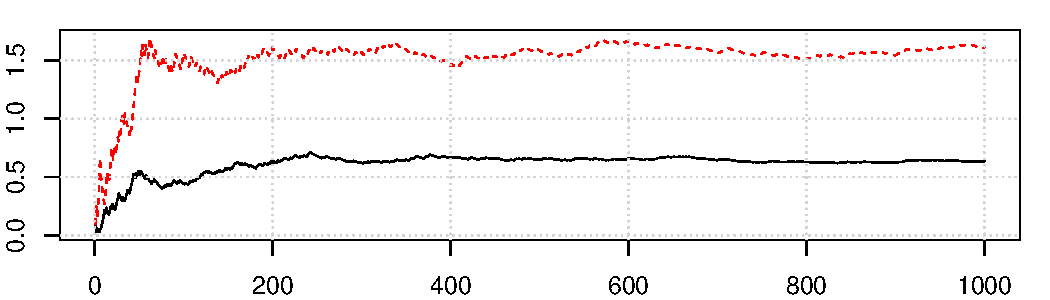
\includegraphics[width=0.98\textwidth]{mhbd2}
	}
	\caption{Metropolis-Hastings algorithm example}
	\label{fig:mhbd}
\end{figure}

%------------------------------------------------------------------------------
% VARIANCE REDUCTION
%------------------------------------------------------------------------------
\section{Variance Reduction}
\label{ap:vr}

The Monte Carlo method consists of sampling a distribution and averaging 
these values to approximate the mean of this distribution. The main drawback 
of this method is the low rate of convergence, on the order $1/\sqrt{N}$.
Variance reduction methods are procedures used to increase the precision 
of the estimates of the Monte Carlo method. The main procedures are common 
random numbers, antithetic variates, control variates, importance sampling 
and stratified sampling.

\subsection{Antithetic variates}
We estimate $E(g(X))$ using the Monte Carlo method. Assume $Y_1$ and 
$Y_2$ as random variables with the identical distribution $g(X)$. 
This indicates that $E(g(X)) = E(Y_1) = E(Y_2) = E(\frac{Y_1+Y_2}{2})$ and
$\text{Var}\left(\frac{Y_1+Y_2}{2}\right) = 
\frac{\text{Var}(Y_1)+\text{Cov}(Y_1,Y_2)}{2}$.
If $Y_1$ and $Y_2$ are negatively correlated, then the variance of $N$ 
simulated values from $\frac{Y_1+Y_2}{2}$ is smaller than the variance 
of $2{\times}N$ simulated values from $Y_1$ or $Y_2$.

\begin{example}
	In this example extracted from 
	\href{http://en.wikipedia.org/wiki/Antithetic_variates}{Wikipedia}, we 
	show how the antithetical method works and how it is used by CCruncher. 
	We would like to estimate the following integral using the Monte Carlo 
	method:
	\begin{displaymath}
		I = \displaystyle \int_0^1 \frac{1}{1+x} \ud x
	\end{displaymath}
	In this case the random variable is $U \sim \text{Uniform}[0,1]$, and 
	its variate is $1-U$. Listing~\ref{sc:antithetic} computes the integral 
	value using plain Monte Carlo, Monte Carlo with antithetic method, and 
	Monte Carlo with antithetic variates but only to reduce the number of 
	simulated values as CCruncher does.
	\\
	\hspace*{1cm}
	\begin{tabular}{l|c|c|c|c|}
		\cline{2-5}
		& Sims & N & Mean & Variance \\
		\hline
		\multicolumn{1}{|l|}{Exact = $\ln(2)$} & - & - & 0.693147 & - \\
		\hline
		\multicolumn{1}{|l|}{Monte Carlo} & 10000 & 10000 & 0.695685 & 0.019624 \\
		\hline
		\multicolumn{1}{|l|}{Antithetic} & 5000 & 5000 & 0.693404 & 0.000593 \\
		\hline
		\multicolumn{1}{|l|}{CCruncher} & 5000 & 10000 & 0.693099 & 0.019508 \\
		\hline
	\end{tabular}
\end{example}
%\vspace{11pt}

\begin{lstlisting}[language=R, label=sc:antithetic, caption=Antithetic example (R script)]

 f <- function(x) { 1/(1+x) }
 
 result = matrix(nrow=4, ncol=4)
 colnames(result) = c("Sims", "N", "Mean", "Variance")
 rownames(result) = 1:4

 rownames(result)[1] = "Exact";
 result[1,1] = 0
 result[1,2] = 0
 result[1,3] = integrate(f, lower=0, upper=1)$value
 result[1,4] = 0

 u = runif(10000)
 rownames(result)[2] = "Monte Carlo";
 result[2,1] = length(u)
 result[2,2] = length(u)
 result[2,3] = mean(f(u))
 result[2,4] = var(f(u))

 u = runif(5000)
 rownames(result)[3] = "Antithetic";
 result[3,1] = length(u)
 result[3,2] = length(u)
 result[3,3] = mean((f(u)+f(1-u))/2)
 result[3,4] = var((f(u)+f(1-u))/2)

 u = runif(5000)
 u = c(u, 1-u)
 rownames(result)[4] = "CCruncher";
 result[4,1] = length(u)/2
 result[4,2] = length(u)
 result[4,3] = mean(f(u))
 result[4,4] = var(f(u))
 
 result

\end{lstlisting}

\subsection{Latin Hypercube Sampling (LHS)}
This variance reduction technique belongs to the stratified sampling family. 
It consists of dividing the total probability range [0,1] in $N$ equispaced 
segments. Then we create a sample of size $N$ picking a random value from 
each segment using a uniform distribution and applying the inverse transform 
sampling. Finally we shuffle the sample to obtain the desired distribution 
random values. When we have two independent random variables, we repeat the 
above procedure for each of them, obtaining the Latin Square effect: the 
generated random points are in a reticle in which each row and column has 
only one point. The procedure for three or more independent variables is 
identical, and it is called Latin Hypercube Sampling~\cite{glasserman:1997}.

When the random variables are dependent, the previous schema does not work, 
and it is reformulated recurring to copulas and the rank statistic~\cite{wolfgang:2008}. 
In this case, the number of bins affects the quality of the generated values, 
the larger the better.

\begin{example}
	We compare the estimated density of $N(0,1)$ using a sample of 100 
	simulated values without using LHS and a sample of 100 simulated values 
	using LHS. Listing~\ref{sc:lhs} exposes the R script, and 
	figure~\ref{fig:lhs} displays the results.
\end{example}

\begin{figure}[!ht]
	\centering
	\subcaptionbox{Empirical cdf (without lhs)}{
		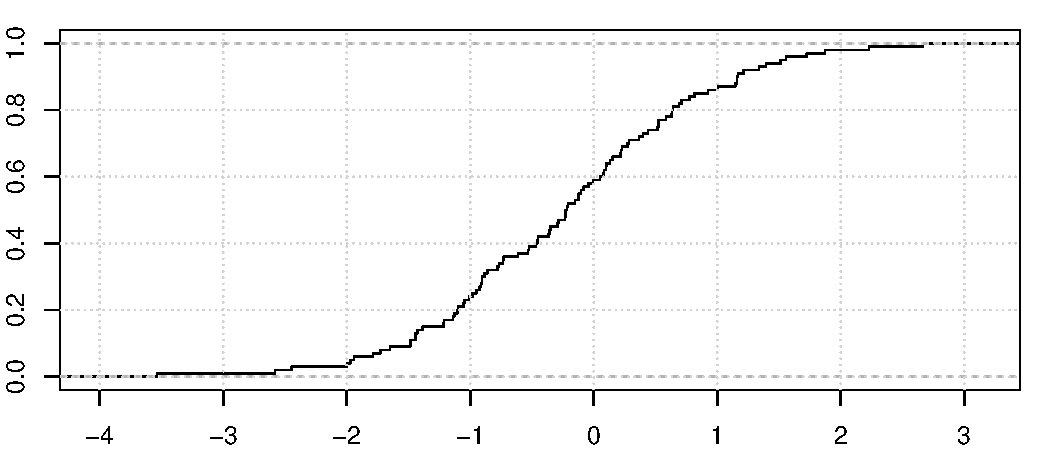
\includegraphics[width=7cm]{lhs1}
	}
	\subcaptionbox{Empirical cdf (using lhs)}{
		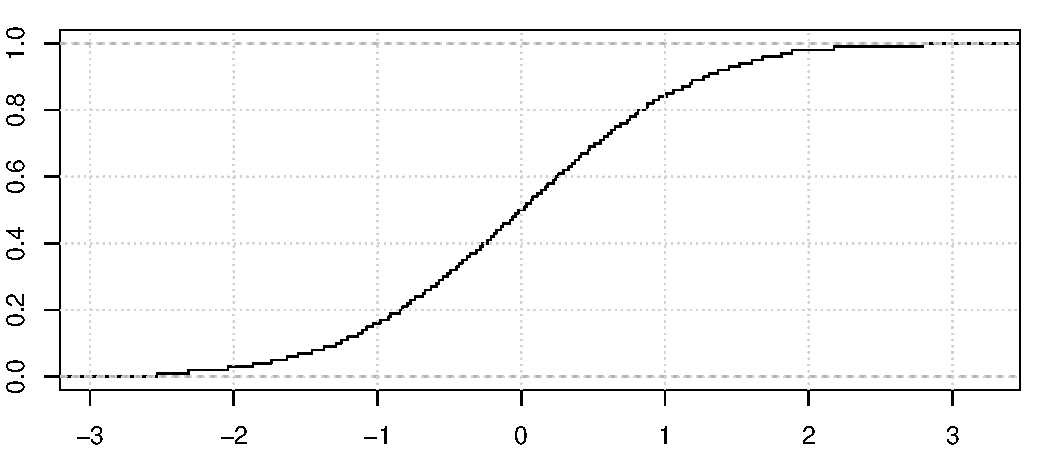
\includegraphics[width=7cm]{lhs2}
	}
	\caption{Latin Hypercube Sampling example (1-dim)}
	\label{fig:lhs} 
\end{figure}

\begin{lstlisting}[language=R, label=sc:lhs, caption=Latin Hypercube Sampling example (R script)]

 rlhs <- function(nblocks, icdf, ...) 
 {
   ret = rep(NA,nblocks)
   for(i in 1:nblocks) {
     u = runif(1, min=(i-1)/nblocks, max=i/nblocks)
     ret[i] = icdf(u, ...)
   }
   ret = sample(ret)
   return(ret)
 }

 x1 = rnorm(100, mean=0, sd=1)
 cdf1 = ecdf(x1)
 plot(cdf1, verticals=TRUE, pch=-1, ylab="prob", main="");
 
 x2 = rlhs(100, qnorm, mean=0, sd=1)
 cdf2 = ecdf(x2)
 plot(cdf2, verticals=TRUE, pch=-1, ylab="prob", main="");
 
\end{lstlisting}


%==============================================================================
% BIBLIOGRAPHY
%==============================================================================
\addcontentsline{toc}{chapter}{\textcolor{ocre}{Bibliography}}
\bibliographystyle{plain}
\bibliography{bibliography}


%----------------------------------------------------------------------------------------

\end{document}
